\documentclass[
 a4paper,
 12pt,
 parskip=half
 ]{scrartcl}

\usepackage{../.tex/settings}

%\usepackage{tabularx}
\usepackage{ltablex}
% X-Spalte wird vertikal zentriert ausgerichtet
\def\tabularxcolumn#1{m{#1}}

\usepackage{../.tex/mathpkgs}
\usepackage{../.tex/mathcmds}

\usepackage{pdfpages}

\usepackage[numbers]{../.tex/fancy_thm}

\theoremstyle{plain}
%\newtheorem{thm}{Satz}[section] % reset theorem numbering for each chapter
\newtheorem*{thm*}{Satz}
%\newtheorem{prp}[thm]{Proposition}
%\newtheorem{lem}[thm]{Lemma}

\theoremstyle{definition}
\newtheorem{defn}[thm]{Definition}
\newtheorem{folg}[thm]{Folgerung}
\newtheorem{exmp}[thm]{}

\newtheorem*{folg*}{Folgerung}
\newtheorem*{exmp*}{Beispiel}
\newtheorem*{defn*}{Definition}
\newtheorem*{deno*}{Bezeichnung}
\newtheorem*{rmrk*}{Bemerkung}

%opening
\title{Vorlesung\\Geometrie}
\subtitle{Wintersemester 2016/2017}
\author{Vorlesung: Prof. Dr. Ulrich Brehm\\Mitschrift: Jonas Hippold}

\hypersetup{
  pdftitle = {Geometrie},
  pdfauthor = {Jonas Hippold},
  hidelinks
}

\begin{document}

\maketitle

\tableofcontents

\clearpage

\setcounter{secnumdepth}{0}
% \section{Einführung}
\subsection{Begriffe der Geometrie}
\begin{itemize}
 \item Felix Klein: Erlanger Programm (1872)
 \item Euklidischer Raum $\real^n$ (mit Standardskalarprodukt)
 \item Isometriegruppe
  \[ f(x) = Ax + t, A \in O(n), t \in \real^n. \]
 \item Kongruenz
  \begin{itemize} 
   \item Alle Geraden sind einander kongruent, ebenso alle Kreise vom selben Radius.
   \item Kongruente Objekte sind durch Invarianten verbunden.
  \end{itemize}
 \item In der Geometrie verwendete Begriffe: Längen, Flächeninhalte, Volumina, Winkel
 \item Winkel sind kongruent, wenn sie die selbe Größe haben.
 \item Kongruenzsätze
 \item Kreis, Invariante Radius
 \item Affine Geometrie, Gruppe: affine Gruppe des $\real^n$
  \[ \{ f: \real^n \to \real^n | f(x) = Ax + t, A \in \GL(n), A \in \realmat{n}{n} \text{ invertierbar}, t \in \real^n. \} \]
 \item Begriffe der affinen Geometrie:
  \begin{itemize}
   \item Geraden
   \item $k$-dimensionale affine Unterräume
   \item Ellipsen
   \item Mittelpunkte von Strecken 
    \[ A \left( \frac{x+y}{2} \right) + t = \frac{A(x) + t}{2} + \frac{A(y) + t}{2} \]
   \item Mittelpunkte von Ellipsen
  \end{itemize}
 \item \emph{Nicht} in der affinen Geometrie: 
  \begin{itemize}
   \item Längen, Winkel
   \item Kreise
   \item Winkelhalbierende
  \end{itemize}
 \item Euklidische Geometrie
 \item Flächeninhalt: Äquiaffine Abbildung
  \[ f(x) = Ax + t, A \in \GL(n), |\det A| = 1 \]
 \item ``Axiomatischer Zugang'' $\longleftrightarrow$ ``Modelle''
\end{itemize}

\subsection{Literatur}
Horst Knörrer: Geometrie (nur eingeschränkt hilfreich)

\subsection{Themen}
\begin{itemize}
 \item Isometrien des $\real^n$, eventuell normale Endomorphismen
 \item Projektive Geometrie
 \item Inversion (Spiegelung) an Sphären und die Möbiusgruppe
 \item Sphärische und hyperbolische (nicht-euklidische) Geometrie
 \item Quadriken
\end{itemize}

\subsection{Bezeichnungen und Konventionen}
\begin{itemize}
 \item Vektoren werden ohne Pfeile geschrieben.
 \item Skalare sind in der Regel griechische Buchstaben
 \item Matrizen werden durch Großbuchstaben bezeichnet.
 \item Wir betrachten oft den $\real^n$, $\complex^n$ mit 
  \begin{itemize}
   \item dem Standardskalarprodukt
    \[ \langle x, y \rangle := \sum_{i=1}^n x_i \bar{y}_i, \]
    wobei $x = (x_1, \ldots, x_n)^T, y = (y_1, \ldots, y_n)^T \in \real^n$ oder $\complex^n$, 
   \item der euklidischen bzw. unitären Norm für $\real^n$ bzw. $\complex^n$
    \[ \| x \| := \sqrt{ \langle x,x \rangle }. \]
  \end{itemize}
 \item Standardbasis des $K^n$ (Körper $K$):
  \[ e_i = \begin{pmatrix} 0 \\ \vdots \\ 0 \\ 1 \\ 0 \\ \vdots \\ 0 \end{pmatrix} \ldots i\text{-te Stelle} \quad (e_1, e_2, \ldots, e_n). \]
 \item Einheitsmatrix des $\real^n$: $E_n$ bzw. $E$, wenn $n$ aus dem Kontext klar ist.
\end{itemize}


\clearpage
\setcounter{secnumdepth}{1}
\section{Isometrien des \texorpdfstring{$\real^n$}{Rn}}
\setcounter{secnumdepth}{0}
Eine Isometrie eines metrischen Raumes $(X, d)$ ist eine bijektive Abbildung $f: X \to X$ mit
\[ d( f(x), f(y) ) = d(x,y) \text{ für alle } x, y \in X. \]

Wir wollen die Isometriegruppe des $(\real^n, d)$ untersuchen mit $d(x,y) := \| x - y \|$.

\begin{thm}
 Sei $V$ ein euklidischer Vektorraum und $g: V \to V$ eine Isometrie. Dann ist $f: V \to V$ mit $f(x) := g(x) - g(0)$ eine orthogonale Abbildung. Insbesondere ist $g$ eine affine Abbildung.
\end{thm}

\begin{proof}
 Sei $f: V \to V$ definiert durch $f(x) := g(x) - g(0)$. Dann folgt $\| f(x) \| = \| g(x) - g(0) \| = \| x - 0 \| = \| x \|$, also
 \begin{align*}
\| f(x_1) - f(x_2) \|^2 
    &= \| f(x_1) \|^2 + \| f(x_2) \|^2 - 2 \langle f(x_1), f(x_2) \rangle \\
    &= \| x_1 \|^2 + \| x_2 \|^2 - 2 \langle f(x_1), f(x_2) \rangle.
 \end{align*}
 Es gilt auch
 \[ \| g(x_1) - g(x_2) \|^2 = \| x_1 - x_2 \| = \| x_1 \|^2 + \| x_2 \|^2 - 2 \langle g(x_1), g(x_2) \rangle, \]
 also bewahrt $f$ auch das Skalarprodukt.
 
 $f$ ist linear:
 \begin{align*} \| f(x_1 + x_2) - f(x_1) - f(x_2) \|^2 
    =\, &\| f(x_1 + x_2) \|^2 
      - 2 \langle f(x_1 + x_2), f(x_1) \rangle \\
    & - 2 \langle f(x_1 + x_2), f(x_2) \rangle
      - 2 \langle f(x_1 ), f(x_2) \rangle \\
    & + \| f(x_1) \|^2 + \| f(x_2) \|^2 \\
    =\, &\| x_1 + x_2 \|^2 
      - 2 \langle x_1 + x_2, x_1 \rangle
      - 2 \langle x_1 + x_2, x_2 \rangle \\
    & - 2 \langle x_1, x_2 \rangle
      + \| x_1 \|^2 + \| x_2 \|^2 \\
    =\, &\| x_1 + x_2 - x_1 - x_2 \|^2 \\
    =\, &0,
 \end{align*}
 also $f(x_1 + x_2) = f(x_1) + f(x_2)$. Es gilt auch
 \begin{align*} \| f(\lambda x) - \lambda f(x) \|^2 &= \| f( \lambda x ) \|^2 
      - 2 \lambda \langle f( \lambda x ), f( x ) \rangle 
      + \lambda^2 \| f(x) \|^2 \\
    &= \| \lambda x \|^2
      - 2 \lambda \langle \lambda x, x \rangle
      + \lambda^2 \| x \|^2 \\
    &= 0,
 \end{align*}
 also $f(\lambda x) = \lambda f(x)$.
 
 Damit ist $f$ eine (bijektive) Abbildung, die das Skalarprodukt bewahrt, also eine orthogonale Abbildung.
\end{proof}

\begin{mydef}[Ähnlichkeitsbegriff]
 Seien $A, B \in \realmat{n}{n}$. $A$ heißt \emph{ähnlich} zu $B$, falls es $S \in \realmat{n}{n}$ gibt, $S$ invertierbar und $B = S^{-1} A S$. Wir schreiben $A \approx B$.
\end{mydef}

\begin{thm}
 Sei $g: V \to V$ eine affine Abbildung mit $\dim V < \infty$ ($V$ euklidischer Vektorraum) und $f: V \to V$ mit $f(x) = g(x) - t$ mit $t := g(0)$ die zugehörige lineare Abbildung.
 
 Falls 1 \emph{kein} Eigenwert von $f$ ist, dann hat $g$ hat genau einen Fixpunkt $x_0$ und lässt sich schreiben als\footnotemark
 \[ g(x) = f(x-x_0) + x_0. \]
\end{thm}
\footnotetext{$f$ ist also im obigen Sinn ähnlich zu $g$.}

\begin{proof}
 Für einen Fixpunkt von $g$ gilt
 \[ g(x_0) = x_0 \,\Leftrightarrow\, f(x_0) + t = x_0 \,\Leftrightarrow\, (\id - f)(x_0) = t \,\Leftrightarrow\, x_0 = (\id - f)^{-1}(t). \]
 Beachte $(\id -f)$ ist bijektiv, da 1 kein Eigenwert von $f$ ist (und $\dim V < \infty$). Also
 \[ f(x - x_0) + x_0 = f(x) + \underbrace{(\id-f)(x_0)}_{t} = f(x) + t = g(x). \]
\end{proof}

Sei $f:\real^n \to \real^n$ und $f(x) = Ax + t$ eine Isometrie, also $A \in O(n)$. Falls 1 Eigenwert von $A$ ist, dann zerlegen wir $t$ in eine Komponente $t_1 \in \ker(A-E)$ und $t_2 \in ker(A-E)^\bot$, $t = t_1 + t_2$. Das heißt, $t_1$ ist die orthogonale Projektion von $t$ auf $\ker(A-E)$ (Fixraum von $A$), $A_2 = t - t_1$.

\begin{bem}
 Falls $(b_1, \ldots, b_n)$ eine Orthonormalbasis von $ker(A-E)$ ist, dann ist also $t_1 = \sum_{i=1}^k \langle t, b_i \rangle b_i$.
\end{bem}

\begin{thm}
 Falls $f: \real^n \to \real^n$ mit $f(x) = Ax + t$, $A \in O(n)$ ist und $t = t_1 + t_2$ mit $t_1 \in \ker(A-E)$, $t_2 \in \ker(A-E)^\bot$, dann ist $f(x) = A(x-x_0) + x_0 + t_1$ für genau ein $x_0 \in \ker(A-E)^\bot$.
\end{thm}

\begin{proof}
 $A$ bildet $\ker(A-E)$ punktweise auf sich selbst ab. Da ferner $A \in O(n)$, bildet $A$ auch $\ker(A-E)^\bot$ auf sich selbst ab, das heißt die Abbildung $\tilde{f}: \ker(A-E)^\bot \to \ker(A-E)^\bot$ mit $\tilde{f}(x) = Ax + t_2 = f(x) - t_1$ ist eine Isometrie von $\ker(A-E)^\bot$, für die die eingeschränkte Abbildung auf diesen Unterraum nicht den Eigenwert 1 hat.
 
 Nach Satz 1.2 hat also $\tilde{f}$ genau einen Fixpunkt in diesem Unterraum und damit gilt
 \[ \tilde{f}(x) = A(x-x_0) + x_0. \qedhere \]
\end{proof}

\subsection{Klassifikation der Isometrien des \texorpdfstring{$\real^2$}{IR2}}
Sei $A \in O(2)$, also $\left(\begin{pmatrix} a_{11} \\ a_{21} \end{pmatrix}, \begin{pmatrix} a_{12} \\ a_{22} \end{pmatrix}\right)$ ist eine Orthonormalbasis des $\real^2$ und $a_{11}^2 + a_{21}^2 = 1$. Dann gibt es $\varphi \in [0,2 \pi)$ mit $a_{11} = \cos \varphi$, $a_{21} = \sin \varphi$ und es ist entweder $\begin{pmatrix} a_{12} \\ a_{22} \end{pmatrix} = \begin{pmatrix} - \sin \varphi \\ \cos \varphi \end{pmatrix}$, falls $\det A = 1$ oder $\begin{pmatrix} a_{12} \\ a_{22} \end{pmatrix} = \begin{pmatrix} \sin \varphi \\ - \cos \varphi \end{pmatrix}$, falls $\det A = -1$.

\begin{enumerate}[1)]
 \item Falls $\det A = 1$ beschreibt $A = \begin{pmatrix} \cos \varphi & - \sin \varphi \\ \sin \varphi & \cos \varphi \end{pmatrix}$ eine Drehung um den Winkel $\varphi$. Die Eigenwerte sind komplex:
 \[ \det \begin{pmatrix} \cos \varphi - \lambda & - \sin \varphi \\ \sin \varphi & \cos \varphi - \lambda \end{pmatrix} = \lambda^2 - 2 \lambda \cos \varphi + 1, \]
 also ist $\lambda_{1,2} = \cos \varphi \pm i \sin \varphi = e^{\pm i \varphi}$.
 
 \emph{Spezialfälle:}
 \begin{enumerate}[a)]
  \item $\varphi = 0$, $A = E$. Die Abbildung $f: \real^2 \to \real^2$ mit $f(x) = x + t$ ist also für $t=0$ die \emph{Identität}, für $t \ne 0$ eine \emph{Translation} um $t$ ($t = t_1$).
  \item $\varphi = \pi$, $A = -E$. Hier ist $f$ eine \emph{Punktspiegelung} (Drehung um $180^\circ = \pi$).
 \end{enumerate}
 Mit $\varphi \ne 0$ beschreibt $f$ nach Satz 1.2 also eine \emph{Drehung}.
 \item Falls $\det A = -1$ hat $A = \begin{pmatrix} \cos \varphi & \sin \varphi \\ \sin \varphi & - \cos \varphi \end{pmatrix}$ reelle Eigenwerte:
 \[ \det \begin{pmatrix} \cos \varphi - \lambda & \sin \varphi \\ \sin \varphi & - \cos \varphi - \lambda \end{pmatrix} = \lambda^2 - 1, \]
 also gilt $\lambda_{1,2} = \pm 1$.
 
 Die affine Abbildung $f(x) = Ax + t_1 + t_2$ mit $t_1 \in \ker(A-E)$, $t_2 \in \ker(A-E)^\bot$ beschreibt für $t_1 = 0$ eine \emph{Spiegelung} an einer Geraden und für $t_1 \ne 0$ eine \emph{Schubspiegelung} an einer Geraden.
\end{enumerate}

\newpage

%\begin{table}[ht]
 {\center \small
 \begin{tabularx}{.95\textwidth}{|>{\center}m{3.5cm}|>{\center}m{3cm}|>{\center}m{3cm}|X|}
  \hline
  Zugehörige lineare Abbildung in Normalform & Isometrie des $\real^2$ & Menge der Fixpunkte & Welche Geraden werden auf sich abgebildet? \\
  \hline
  $\begin{pmatrix} 1 & 0 \\ 0 & 1 \end{pmatrix}$ &
  Identität, falls $t = t_1 = 0$, &
  $\real^2$ &
  Alle Geraden \\
   & Translation, falls $t = t_1 \ne 0$
   & $\emptyset$
   & Alle Geraden parallel zu $\real t$ \\  
  \hline
  $\begin{pmatrix} -1 & 0 \\ 0 & -1 \end{pmatrix}$ &
  Punktspiegelung an $p = \frac{t}{2}$ (Drehung in $p$ um den Winkel $\pi$) &
  $\{p\}$ &
  Alle Geraden durch $p$ \\
  \hline
  $\begin{pmatrix} \cos \varphi & - \sin \varphi \\ \sin \varphi & \cos \varphi \end{pmatrix}$ &
  Drehung um einen Punkt $p$ um Winkel $\ne 0, \pi$ &
  $\{p\}$ &
  keine \\
  \hline
  $\begin{pmatrix} 1 & 0 \\ 0 & -1 \end{pmatrix}$ &
  Spiegelung an einer Geraden $g$, falls $t_1 = 0$  &
  $g$ &
  $g$ und alle Geraden orthogonal zu $g$ \\
   & Schubspiegelung an $g$, falls $t_1 \ne 0$
   & $\emptyset$
   & $g$ \\
   \hline
 \end{tabularx} }
 \[ x \mapsto Ax + t, t = t_1 + t_2 \text{ mit } t_1 \in \ker(A-E), t_2 \in \ker(A-E)^\bot \]
% \caption{Klassifikation der Isometrien des $\real^2$}
%\end{table}

Vorschlag zum zusätzlichen Selbststudium: Die 17 kristallographischen Gruppen der Ebene

\newpage

\subsection{Isometrien des \texorpdfstring{$\real^3$}{IR3}}
Zunächst sei $A \in O(3)$ eine orthogonale $3 \times 3$-Matrix. Das charakteristische Polynom $\chi_A$ ist vom Grad 3, hat also mindestens eine reelle Nullstelle. Ferner haben alle reellen oder komplexen Nullstellen den Betrag 1.

Falls das charakteristische Polynom über $\real$ in Linearfaktoren zerfällt, gibt es eine Orthonormalbasis des $\real^3$ aus Eigenvektoren von $A$ und die Matrix $A$ ist \emph{bezüglich dieser Basis} von der Form 
\begin{align*}
 \begin{pmatrix} 1 & 0 & 0 \\ 0 & 1 & 0 \\ 0 & 0 & 1 \end{pmatrix} &\text{ (Identität) oder} \\
 \begin{pmatrix} 1 & 0 & 0 \\ 0 & 1 & 0 \\ 0 & 0 & -1 \end{pmatrix} &\text{ (Spiegelung an einer Ebene) oder} \\
 \begin{pmatrix} 1 & 0 & 0 \\ 0 & -1 & 0 \\ 0 & 0 & -1 \end{pmatrix} &\text{ (Spiegelung an einer Geraden) oder} \\
 \begin{pmatrix} -1 & 0 & 0 \\ 0 & -1 & 0 \\ 0 & 0 & -1 \end{pmatrix} &\text{ (Punktspiegelung)}.
\end{align*}
Andernfalls hat $A$ einen reellen Eigenwert $\pm 1$ und $\chi_A$ hat ferner konjugiert komplexe Nullstellen $\cos \varphi \pm i \sin \varphi$ mit $\varphi \ne 0, \pi$, $\varphi \in [0, 2\pi)$.

Sei $b_1$ der Eigenvektor zum Eigenwert $\pm 1$ mit $\| b_1 \| = 1$. Ergänze zu einer Orthonormalbasis $b_1, b_2, b_3$. Dann ist die Matrix $A$ bezüglich dieser Basis eine orthogonale Matrix und von der Form 
\[ \begin{pmatrix} 1 & 0 & 0 \\ 0 & \cos \varphi & -\sin \varphi \\ 0 & \sin \varphi & \cos \varphi \end{pmatrix}
   \text{ oder }
   \begin{pmatrix} -1 & 0 & 0 \\ 0 & \cos \varphi & -\sin \varphi \\ 0 & \sin \varphi & \cos \varphi \end{pmatrix}. \]
Im ersten Fall ($\det A = 1$) ist die lineare Abbildung eine \emph{Drehung} um die Gerade $\real b_1$ um den Winkel $\varphi$. Im zweiten Fall ($\det A = -1$) ist es eine \emph{Drehspiegelung} mit der \emph{Drehspiegelachse} $\real b_1$ mit \emph{Drehspiegelebene} $\real b_2 + \real b_3$ um den Winkel $\varphi$.

%\begin{table}[ht]
 {\center \small
 \begin{tabularx}{.95\textwidth}{|>{\center}m{3.6cm}|>{\center}m{3cm}|>{\center}m{3cm}|X|}
  \hline
  Zugehörige lineare Abbildung in Normalform 
   & Isometrie des $\real^3$ 
   & Menge der Fixpunkte 
   & Welche Geraden werden auf sich abgebildet? \\
  \hline
  $\begin{pmatrix} 1 & 0 & 0 \\ 0 & 1 & 0 \\ 0 & 0 & 1 \end{pmatrix}$ 
   & Identität, falls $t = t_1 = 0$, 
   & $\real^3$ 
   & Alle Geraden \\
   & Translation, falls $t = t_1 \ne 0$
   & $\emptyset$
   & Alle Geraden parallel zu $\real t$ \\  
  \hline
  $\begin{pmatrix} 1 & 0 & 0 \\ 0 & -1 & 0 \\ 0 & 0 & -1 \end{pmatrix}$
   & Spiegelung an einer Geraden, falls $t_1 = 0$ (Drehung um $\pi$),
   & $g$
   & $g$ und alle Geraden, die $g$ orthogonal schneiden. \\
   & Gleitspiegelung an einer Geraden, falls $t_1 \ne 0$ (Schraubung um $\pi$)
   & $\emptyset$
   & $g$ \\
  \hline
  $\begin{pmatrix} 1 & 0 & 0 \\ 0 & \cos \varphi & - \sin \varphi \\ 0 & \sin \varphi & \cos \varphi \end{pmatrix}$ 
   & Drehung an einer Geraden, falls $t_1 = 0$ 
   & $g$
   & $g$ \\
   & Schraubung, falls $t_1 \ne 0$
   & $\emptyset$
   & $g$ \\
  \hline
  $\begin{pmatrix} -1 & 0 & 0 \\ 0 & -1 & 0 \\ 0 & 0 & -1 \end{pmatrix}$
   & Punktspiegelung am Punkt $p=\frac{t}{2}$
   & $p$
   & Alle Geraden durch $p$ \\
  \hline
  $\begin{pmatrix} 1 & 0 & 0 \\ 0 & 1 & 0 \\ 0 & 0 & -1 \end{pmatrix}$
   & Spiegelung an einer Ebene $E$, falls $t_1 = 0$
   & $E$
   & Alle Geraden in $E$ und alle Geraden $\bot E$ \\
   & Gleitspiegelung an einer Ebene, falls $t_1 \ne 0$.
   & $\emptyset$
   & Alle Geraden in $E$ parallel zu $\real t$ \\
  \hline
  {\footnotesize $\begin{pmatrix} -1 & 0 & 0 \\ 0 & \cos \varphi & - \sin \varphi \\ 0 & \sin \varphi & \cos \varphi \end{pmatrix}$}
   & Drehspiegelung mit Drehspiegelachse $g$ und Fixpunkt $p$
   & $p$
   & $g$ \\
  \hline
 \end{tabularx} }
 \[ x \mapsto Ax + t, A \in O(3), t = t_1 + t_2 \text{ mit } t_1 \in \ker(A-E), t_2 \in \ker(A-E)^\bot \]
 %\caption{Klassifikation der Isometrien des $\real^3$}
%\end{table}

\begin{bem}[Orientierung bei Drehungen]
Äquivalenz über $S \in SO(n)$, das heißt $\det S=1$ statt mit $S \in O(n)$. 
 
 In $\real^2$ ist dann $\varphi$ eindeutig bestimmt:
 \[ S \begin{pmatrix} \cos \varphi & - \sin \varphi \\ \sin \varphi & \cos \varphi \end{pmatrix} S^{-1} = \begin{pmatrix} \cos \varphi & - \sin \varphi \\ \sin \varphi & \cos \varphi \end{pmatrix}, \]
 falls $S \in SO(2)$. Für $S \in O(2) \setminus SO(2)$ zum Beispiel
 \[ \begin{pmatrix} -1 & 0 \\ 0 & 1 \end{pmatrix}
    \begin{pmatrix} \cos \varphi & - \sin \varphi \\ \sin \varphi & \cos \varphi \end{pmatrix}
    \begin{pmatrix} -1 & 0 \\ 0 & 1 \end{pmatrix}
    = 
    \begin{pmatrix} \cos (-\varphi) & - \sin (-\varphi) \\ \sin (-\varphi) & \cos (-\varphi) \end{pmatrix} \]
 
 Bei Drehungen in $\real^3$ kann man (geometrisch) nicht zwischen Drehung um $\varphi$ und $-\varphi$ unterscheiden:
 \[ \begin{pmatrix} -1 & 0 & 0 \\ 0 & -1 & 0 \\ 0 & 0 & 1 \end{pmatrix}
    \begin{pmatrix} -1 & 0 & 0 \\ 0 & \cos \varphi & - \sin \varphi \\ 0 & \sin \varphi & \cos \varphi \end{pmatrix}
    \begin{pmatrix} -1 & 0 & 0 \\ 0 & -1 & 0 \\ 0 & 0 & -1 \end{pmatrix}
    =
    \begin{pmatrix} -1 & 0 & 0 \\ 0 & \cos \varphi & \sin \varphi \\ 0 & -\sin \varphi & \cos \varphi \end{pmatrix}.
 \]
 Bei Drehspiegelungen ist das genauso.
 
 Im Gegensatz dazu: bei Schraubungen wähle den Basisvektor $b_1 \in \ker(A-E)$ (mit $\|b_1\| = 1$), so dass $t_1 = \lambda b_1$ mit $\lambda > 0$. Dann ist $\varphi$ auch eindeutig bestimmt (in der Drehebene, vgl. $\real^2$).
\end{bem}

\subsection{Normale Endomorphismen des \texorpdfstring{$\real^n$}{IRn}}
\begin{mydef}
Sei $V$ ein unitärer oder euklidischer Raum mit Skalarprodukt $\langle \cdot, \cdot \rangle$ und $f:V \to V$ ein Endomorphismus. Falls $f^*:V \to V$ ein Endomorphismus ist, sodass für alle $x,y \in V$ gilt
\[ \langle f(x), y \rangle = \langle x, f^*(y) \rangle, \]
dann heißt $f^*$ der \emph{zu $f$ adjungierte} Endomorphismus (bezüglich $\langle \cdot, \cdot \rangle$). Falls er existiert, dann ist er eindeutig bestimmt.

Falls $\dim V < \infty$, dann existiert $f^*$ immer und es gilt: Falls $A$ die Matrix von $f$ bezüglich einer Orthonormalbasis ist, dann ist $A^* = \obar{A}^T$ die Matrix von $f^*$ bezüglich derselben Basis.

Ein Endomorphismus $f$ heißt \emph{normal}, falls $f^*$ existiert und $f f^* = f^* f$ gilt. Eine Matrix $A \in \compmat{n}{n}$ heißt \emph{normal}, falls $A^* A = A A^*$ gilt.
\end{mydef}

\begin{thm}[Normalform für normale Matrizen]
 Sei $A \in \compmat{n}{n}$, dann sind die folgenden Aussagen äquivalent:
 \begin{enumerate}[(1)]
  \item Es gibt eine Orthonormalbasis aus Eigenvektoren von $A$.
  \item $A$ ist normal.
  \item $A$ ist unitär ähnlich zu einer Diagonalmatrix, das heißt es gibt eine unitäre Matrix\footnotemark\, $S$ mit $S^{-1} A S = D$, $D$ Diagonalmatrix.
 \end{enumerate}
\end{thm}
\footnotetext{$S \in U(S)$: Zeilen- und Spaltenvektoren sind orthonormal bzgl. des Standardskalarprodukts, $S^{-1} = S^*$.}

\begin{folg}
 Sei $A \in \compmat{n}{n}$, dann sind äquivalent:
 \begin{enumerate}[(1)]
  \item $A = A^*$.
  \item $A$ ist normal und alle Eigenwerte von $A$ sind reell.
 \end{enumerate}
\end{folg}

\begin{folg}
 Sei $A \in \compmat{n}{n}$, dann sind äquivalent:
 \begin{enumerate}[(1)]
  \item $A^* = A^{-1}$, das heißt $A \in U(n)$.
  \item $A$ ist normal und alle Eigenwerte von $A$ haben Betrag 1.
 \end{enumerate}
\end{folg}

\begin{lem}
 Sei $A \in \realmat{n}{n} \subset \compmat{n}{n}$. Dann gilt für $A$ als Matrix in $\compmat{n}{n}$ aufgefasst: Falls $x \in \complex^n$ ein Eigenvektor von $A$ zum Eigenwert $c \in \complex$ ist, dann ist $\obar{x}$ ein Eigenvektor von $A$ zum Eigenwert $\obar{c}$, wobei
 \[ \obar{\begin{pmatrix} x_1 \\ \vdots \\ x_n \end{pmatrix}} := \begin{pmatrix} \obar{x}_1 \\ \vdots \\ \obar{x}_n \end{pmatrix}. \]
\end{lem}

\begin{proof}
 Für $x \ne 0$ gilt $Ax = cx $ $\Rightarrow$  $A\obar{x} = \obar{A}\obar{x} = \obar{Ax} = \obar{cx} = \obar{c} \obar{x}$.
\end{proof}

\begin{thm}[Normalform für über $\complex$ diagonalisierbare Matrizen]
 Sei $A \in \realmat{n}{n}$ und $A$ als Element von $\compmat{n}{n}$ aufgefasst diagonalisierbar\footnotemark. Dann gibt es eine Matrix $S \in \GL(n, \real)$ für welche $S^{-1} A S$ die Gestalt
 \[ S^{-1} A S = \begin{pmatrix}
     d_1 &        &     &     &        &      \\
         & \ddots &     &     & 0      &      \\
         &        & d_k &     &        &      \\
         &        &     & \boxed{z_1} &        &      \\
         & 0      &     &     & \ddots &      \\
         &        &     &     &        & \boxed{z_m}
    \end{pmatrix} \]
 hat, wobei $z_\mu = \begin{pmatrix} a_\mu & b_\mu \\ -b_\mu & a_\mu \end{pmatrix}$ für $\mu = 1, \ldots, m$ ist mit $b_\mu \ne 0$, $k+2m = n$. Dabei sind $d_1, \ldots, d_k$ die reellen Eigenwerte von $A$ und $a_\mu \pm i b_\mu$ die komplexen Eigenwerte von $A$ (mit Vielfachheiten).
 
 Ferner gilt: Falls $A$ normal ist, dann kann $S \in O(n)$ gewählt werden, das heißt $S^T = S^{-1}, S \in \realmat{n}{n}$).
\end{thm}
\footnotetext{$A$ ist zu einer Diagonalmatrix $D$ ähnlich, also ex. $S$, so dass $D=S^{-1} A S$.}

\begin{proof}
 Das charakteristische Polynom $\chi_A = \det ( XE - A )$ zerfällt über $\complex$ in Linearfaktoren. Da $A \in \realmat{n}{n}$ ist $\det(XE-A)$ ein Polynom mit reellen Koeffizienten und die Nullstellen kommen reell oder in Paaren komplex konjugierter Zahlen vor.
 
 Wir können also die Nullstellen (unter Berücksichtigung der Vielfachheit) sortieren als
 \[ d_1, \ldots, d_n, a_1 + i b_1, a_1 - i b_1, \ldots, a_m + i b_m, a_m - i b_m \]
 mit $d_\mu, a_\mu, b_\mu \in \real$, $b_\mu \ne 0$.
 
 Da $A$ über $\complex$ diagonalisierbar ist, gibt es eine Basis von Eigenvektoren. Falls $u_1, \ldots, u_r$ eine Basis von (komplexem) Eigenvektoren und $A$ zu einem nicht-reellen Eigenwert $a + ib$ von $A$ ist, dann sind $\obar{u}_1, \ldots, \obar{u}_r$ (nach Lemma 1.4) eine Basis von Eigenvektoren zum Eigenwert $a - ib$. 
 
 Falls $A$ normal\footnote{$A^T A = A A^T$} ist, dann gibt es nach Satz 1.1 sogar eine komplexe Orthonormalbasis\footnote{$\scalar{\obar{u}_i, \obar{u}_j} = \scalar{u_i, u_j} = \delta_{ij}$} von Eigenvektoren. Wähle in diesem Fall $u_1, \ldots, u_r$ als Orthonormalbasis von Eigenvektoren von $A$ zum Eigenwert $a+ib$. $\obar{u}_1, \ldots, \obar{u}_r$ sind dann eine Orthonormalbasis von Eigenvektoren zum Eigenwert $a-ib$. 
 
 Man erhält die gewünschte Basis folgendermaßen: Für die reellen Eigenwerte wähle reelle Eigenvektoren (als Orthonormalsystem bei normaler Matrix $A$). Für ein Paar komplex konjugierter Eigenwerte $a \pm ib$ wähle als Basisvektoren
 \[ \rez{\sqrt{2}} ( u_1 + \obar{u}_1 ), \rez{\sqrt{2}} (\obar{u}_1 - u_1), \ldots, 
    \rez{\sqrt{2}} ( u_r + \obar{u}_r ), \rez{\sqrt{2}} (\obar{u}_r - u_r). \]
 Das sind Vektoren aus $\real^n$ ($\sqrt{2} \cdot$ Realteil von $u_\mu$, $\sqrt{2} \cdot$ Imaginärteil von $u_\mu$). Dann gilt
 \begin{align*}
 A \left( \rez{\sqrt{2}} ( u_1 + \obar{u}_1 ) \right) 
      &= \rez{\sqrt{2}} ( (a +ib) u_1 - (a-ib) \obar{u}_1 ) \\
      &= a \left( \rez{\sqrt{2}} ( u_1 + \obar{u}_1 ) \right ) 
       - b \left( \frac{i}{\sqrt{2}}( \obar{u}_1 - u_1 ) \right),
 \end{align*}
 \begin{align*}
  A \left( \rez{\sqrt{2}} ( \obar{u}_1 - u_1 ) \right) 
      &= \frac{i}{\sqrt{2}} ( (a -ib) \obar{u}_1 - (a+ib) u_1 ) \\
      &= b \left( \rez{\sqrt{2}} ( u_1 + \obar{u}_1 ) \right ) 
       + a \left( \frac{i}{\sqrt{2}}( \obar{u}_1 - u_1 ) \right).
 \end{align*}
 Damit erhalten wir also die reelle $2 \times 2$-Matrix $\begin{pmatrix} a & b \\ -b & a \end{pmatrix}$, entsprechend für die anderen Paare von Eigenvektoren. Damit ist die behauptete Normalform gezeigt.
 
 Wir erhalten im Fall von normalen Matrizen eine reelle Orthonormalbasis, denn zu verschiedenen (komplexen) Eigenwerten sind die (komplexen) Eigenräume orthogonal (uni\-täres Standardskalarprodukt auf $\complex^n$. Die Eigenvektoren haben Betrag 1:
 \[ \left\| \rez{\sqrt{2}} ( u_1 + \obar{u}_1 ) \right\| = \scalar{\rez{\sqrt{2}} ( u_1 + \obar{u}_1 ), \rez{\sqrt{2}} ( u_1 + \obar{u}_1 )} = 1, \]
 da $\| u_1 \| = \| \obar{u}_1 \| = 1$ und $\scalar{\obar{u}_1, u_1} = 0$. Genauso
 \[ \left\| \frac{i}{\sqrt{2}} ( u_1 - \obar{u}_1 ) \right\| = 1. \]
 Nun zeigen wir die paarweise Orthogonalität:
 \[ \scalar{\rez{\sqrt{2}} (u_1 + \obar{u}_1), \frac{i}{\sqrt{2}} (\obar{u}_1 - u_1)} = \frac{i}{\sqrt{2}} \scalar{u_1, u_1} - \frac{i}{\sqrt{2}} \scalar{\obar{u}_1, \obar{u}_1} = 0 \]
 Bei mehrfachen komplexen Eigenwerten hatten wir eine Orthonormalbasis gewählt, also gilt zum Beispiel
 \[ \scalar{\rez{\sqrt{2}} ( u_1 + \obar{u}_1 ), \rez{\sqrt{2}} ( u_k + \obar{u}_k )} = 0, \]
 wegen $\scalar{u_1, u_k} = 0$ (auch für $\scalar{u_1, \obar{u}_k}, \ldots$).
 
 Insgesamt haben wir also eine reelle Orthonormalbasis gefunden, bezüglich der die normale Matrix $A$ die gewünschte Normalform hat.
\end{proof}

\subsection{Geometrische Interpretation}
Sei $z = a \pm ib = |z| e^{\pm i \varphi} = |z| ( \cos \varphi \pm i \sin \varphi)$ ein paar komplex konjugierter Eigenwerte von $A$ mit $b \ne 0$. Die zugehörige $2 \times 2$-Matrix
\[ \begin{pmatrix} |z| \cos \varphi & - |z| \sin \varphi \\ |z| \sin \varphi & |z| \cos \varphi \end{pmatrix}
   = |z| \begin{pmatrix} \cos \varphi & - \sin \varphi \\ \sin \varphi & \cos \varphi \end{pmatrix} \]
beschreibt eine \emph{Drehstreckung} mit Streckungsfaktor $|z| = \sqrt{a^2 + b^2}$ und Drehwinkel $\varphi$ (mit $\varphi \ne 0, pi$).

\textbf{Folgerung aus Satz 1.8:}
\begin{thm}{}
 \begin{enumerate}[a)]
  \item Sei $A \in O(n)$ und $k = \dim \ker(A-E)$. Dann lässt sich $A$ als Produkt von $n-k$ Spiegelungen an Hyperebenen schreiben.
  \item Jede Isometrie des $\real^n$ lässt sich als Produkt von höchstens $n+1$ Spiegelungen an (affinen) Hyperebenen schreiben.
 \end{enumerate}
\end{thm}

%Aufgabe: Was ist geometrisch das Produkt von zwei Spiegelungen an windschiefen Geraden des $\real^n$?

%Betrachte die zugehörigen linearen Abbildungen: Es ergibt sich eine Drehung um den doppelten Winkel des Winkels zwischen $g_1$ und $g_2$.

\clearpage
\setcounter{secnumdepth}{1}
\section{Projektive Geometrie}
\setcounter{secnumdepth}{0}
$(P,G,I)$: $P$, $G$ Mengen, $I \subseteq P \times G$.

$P$: Menge der Punkte \\
$G$: Menge der Geraden \\
$I$: Inzidenzrelation.

Schreib- und Sprechweisen:
\begin{itemize}
 \item Statt $(p,g) \in I$ schreibe $pIg$, ``$p$ liegt auf $g$''. 
 \item Zwei Geraden $g_1$, $g_2$ ``schneiden sich in $p$'' heißt $pIg_1$ und $pIg_2$. 
 \item Drei Punkte $p_1$, $p_2$, $p_3$ heißen ``kollinear'', falls es $g \in G$ gibt, so dass $p_1$, $p_2$, $p_3$ auf $g$ liegen.
 \item Für $g_1, g_2 \in G$ ist
  \[ g_1 \cap g_2 = \begin{cases}
                   p, &\text{falls sich } g_1, g_2 \text{ in } p \text{ schneiden.} \\
                   \emptyset, &\text{falls sie sich nicht schneiden.} \\
                   g_1 = g_2, &\text{falls die Geraden zusammen fallen.}
                  \end{cases} \]
\end{itemize}

\subsection{Projektiver Raum}
\begin{defn*}\label{def:proj}
 Ein \emph{projektiver Raum} $\proj = (P,G,I)$ besteht aus zwei Mengen $P$, $G$ und einer Relation $I \subseteq P \times G$, sodass gilt:
 \begin{enumerate}[\hspace{.5cm}{A}1)]
  \item Durch je zwei (verschiedene) Punkte $p_1$, $p_2$ geht genau eine Gerade. Bezeichne diese Gerade mit $p_1 p_2$.
  \item Sind $p_1$, $p_2$, $p_3$, $p_4$ vier Punkte, sodass sich die Geraden $p_1 p_2$ und $p_3 p_4$ schneiden, dann treffen sich auch $p_1 p_3$ und $p_2 p_4$.
  \item Auf jeder Geraden liegen mindestens drei Punkte.
  \item Es gibt mindestens zwei Geraden.
 \end{enumerate}
\end{defn*}

\begin{defn*}
 Der projektive Raum $\proj = (P,G,I)$ heißt eine \emph{projektive Ebene}\footnote{Die Zeichenebene ist keine projektive Ebene! Zum Beispiel kann man in A2 $p_1$, $p_2$, $p_3$, $p_4$ so wählen, dass $p_1 p_3$ und $p_2 p_4$ parallel sind.}, falls die folgende Verschärfung von A2 gilt:
 \begin{enumerate}[\hspace{.5cm}{A}1)]
  \item [A2')] Je zwei Geraden schneiden sich.
 \end{enumerate}
\end{defn*}

\begin{bem}
 Aus A1 folgt: Falls Geraden $g_1$, $g_2$ mindestens zwei Punkte $p_1$, $p_2$ gemeinsam haben, dann folgt $g_1 = g_2$. Das heißt zwei (verschiedene) Geraden $g_1$, $g_2$ schneiden sich in höchstens einem Punkt.
\end{bem}

Erinnerung: In einem Schiefkörper $(K, +, \cdot)$ gelten alle Körperaxiome, bis auf die Kommutativität von $\cdot$. Also ist $(K, +)$ eine abelsche Gruppe (mit neutralem Element $0$) und $(K \setminus \{ 0 \}, \cdot)$ ist eine Gruppe (mit neutralem Element 1). Es gelten die Distributivgesetze:
\begin{align*}
 a(b+c) = ab + ac, \\
 (a+b)c = ac + bc.
\end{align*}

Im (Links-)Vektorraum $V$ über dem Schiefkörper $K$ gelten alle Axiome außer, dass der Skalarbereich ein Schiefkörper ist, zum Beispiel $\lambda( \mu x ) = (\lambda \mu) x$, $\lambda, \mu \in K$, $x \in V$.

Wenn man eine lineare Abbildung durch Matrizen beschreiben will, besser Rechtsvektorraum $A(x\lambda) = (Ax) \lambda$.

\begin{bem}
 Grundlegendes aus der linearen Algebra gilt auch für Vektorräume über Schiefkörpern (z.B. Basis, Dimension, Dimensionssatz). Determinanten sind nicht vernünf\-tig definierbar und alles was mit ihnen zusammenhängt gilt damit auch nur eingeschränkt.
\end{bem}

\begin{defn*}
 Ein \emph{echter Schiefkörper} $K$ ist ein Schiefkörper, bei dem die Multiplikation \emph{nicht} kommutativ ist.
\end{defn*}

Sei $K$ ein Schiefkörper, $V$ ein (Links-)$K$-Vektorraum. Definiere
\begin{itemize}
 \item $P := \{ Kx | x \in V \setminus \{ 0 \} \}$ Menge der 1-dimensionalen linearen Unterräume,
 \item $G := \{ Kx + Ky | x, y \in V $ linear unabhängig $\}$ Menge der 2-dimensionalen linearen Unterräume.
 \item $p I G \Leftrightarrow p \subseteq g$, $p$ liegt auf $g$, wenn falls der 1-dimensionale Unterraum $p$ in $g$ enthalten ist.
\end{itemize}

\begin{defn*}
 $\proj(V) := (P,G,I)$.
\end{defn*}

\begin{deno*}
 $[x] := Kx$ (für $x \in V \setminus \{ 0 \}$), $[x,y] := Kx + Ky$ ist die lineare Hülle von $x,y$.
\end{deno*}

\begin{thm}
 Falls $V$ ein $K$-Vektorraum über einem Schiefkörper $K$ mit $\dim V \ge 3$ ist, dann ist $\proj(V)$ ein projektiver Raum. Ist $\dim V = 3$, dann ist $\proj(V)$ eine projektive Ebene.
\end{thm}

\begin{proof}
 A1) Für $[x], [y] \in P$ mit $[x] \ne [y]$ gilt $x,y$ sind linear unabhängig und damit ist $[x,y]$ der einzige zweidimensionale Unterraum, der $[x]$ und $[y]$ enthält.
 
 A2) Seien $p_1 = [x_1]$, $p_2 = [x_2]$, $p_3 = [x_3]$, $p_4 = [x_4] \in P$ vier verschiedene Punkte, sodass sich $p_1 p_2 = [x_1, x_2]$ und $p_3 p_4 = [x_3, x_4]$ treffen. Dann ist $\dim ( [x_1 x_2] \cap [x_3 x_4] ) \ge 1$ und wir erhalten mit der Dimensionsformel:
 \begin{align*}
  \dim( [x_1, x_2, x_3, x_4]) &= \dim( [x_1, x_2] ) + \dim( [x_3, x_4] ) - \dim( [x_1,x_2] \cap [x_3,x_4] ) \\
  &\le 2+2-1 = 3.
 \end{align*}
 Nun benutzen wir nochmals die Dimensionsformel, um $\dim( [x_1,x_3] \cap [x_2,x_4] )$ abzuschätzen:
 \begin{align*}
  \dim( [x_1,x_3] \cap [x_2,x_4] ) &= \dim( [x_1, x_3] ) + \dim( [x_2, x_4] ) - \dim( [x_1, x_2, x_3, x_4]) \\
  &\ge 2 + 2 - 3 = 1.
 \end{align*}
 Also treffen sich auch $p_1 p_3$ und $p_2 p_4$.
 
 A3) Sei $[x,y] \in G$, also $\{ x,y \}$ linear unabhängig, dann sind auch $\{ x, x+y \}$ und $\{ y, x+y \}$ linear unabhängig, also $[x]$, $[y]$, $[x+y]$ drei verschiedene Punkte auf $[x,y]$.
 
 A4) Da $\dim V \ge 3$ gibt es linear unabhängige Vektoren $x,y,z \in V$. Damit ist $[x,y] \ne [y,z]$ (beide in $G$).
 
 A2') Falls $\dim V = 3$, $g_1, g_2 \in G$, $g_1 \ne g_2$, dann gilt 
 \[ \dim( g_1 \cap g_2 ) = \dim g_1 + \dim g_2 - \dim( g_1 + g_2 ) = 2 + 2 - 3 = 1. \qedhere \]
\end{proof}

\begin{defn*}
 Unter einem \emph{Dreieck} verstehen wir ein Tripel $(A_1, A_2, A_3)$ von nicht kollinearen Punkten. $A_1, A_2, A_3$ heißen die \emph{Ecken}, $A_2 A_3, A_1 A_3, A_1 A_2$ heißen die \emph{Seiten} des Dreiecks.
\end{defn*}

\subsection{Satz von Desargues}
\begin{defn*}
 Sei $\proj$ ein projektiver Raum. $\proj$ heißt \emph{desarguessch} (oder in $\proj$ gilt der Satz von Desargues), falls für je zwei Dreiecke $(A_1, A_2, A_3)$, $(B_1, B_2, B_3)$, bei denen die einander entsprechenden Ecken und Seiten verschieden sind, gilt: 
 \begin{addmargin}[.5cm]{0cm}
 Wenn die drei Verbindungsgeraden durch die einander entsprechenden Ecken durch einen Punkt gehen, dann sind die drei Schnittpunkte der einander entsprechenden Seiten kollinear. 
 \end{addmargin}
 Also:
 \begin{addmargin}[.5cm]{0cm}
 Falls es $Z \in P$ gibt mit $z = A_1 B_1 \cap A_2 B_2 \cap A_3 B_3$, dann sind
 \[ P_{12} := A_1 A_2 \cap B_1 B_2, \quad P_{13} := A_1 A_3 \cap B_1 B_3, \quad P_{23} := A_2 A_3 \cap B_2 B_3 \]
 kollinear.
 \end{addmargin}

 Falls die 10 Punkte $Z, A_1, A_2, A_3, B_1, B_2, B_3, P_{12}, P_{13}, P_{23}$ und 10 Geraden\footnote{Die sechs Seiten der Dreiecke, die drei Verbindungsgeraden und die Gerade, auf der $P_{12}, P_{13}, P_{23}$ liegen.}  paarweise verschieden sind, nennt man diese Konfiguration aus 10 Punkten und 10 Geraden die \emph{Konfiguration von Desargues}.
\end{defn*}

\begin{figure}[ht]
 \center
 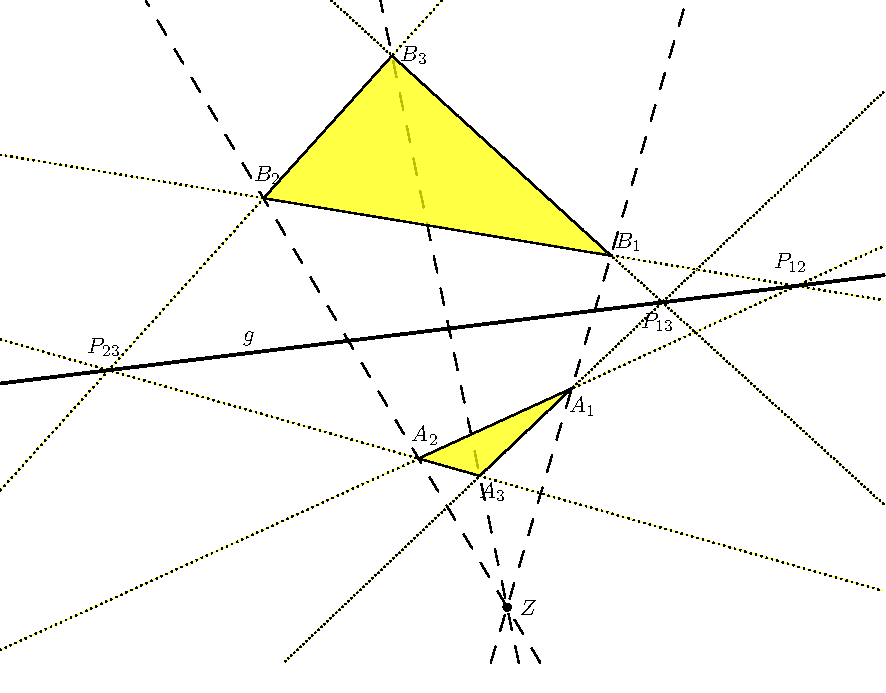
\includegraphics[width=12cm]{img/desargues}
\end{figure}

\begin{thm}
 Sei $V$ ein $K$-Vektorraum über einem Schiefkörper $K$ mit $\dim V \ge 3$. Dann ist $\proj(V)$ desarguessch.
\end{thm}

\begin{proof}
 Falls $Z$ mit einer Ecke übereinstimmt ist die Behauptung trivial. Sei also o.B.d.A. $Z \ne A_i$, $Z \ne B_i$, $A_i \ne B_i$ für $i = 1,2,3$. Seien $Z = [v]$, $A_i = [v_i]$. 
 
 Wir können nun $B_i = [v + v_i]$, $i = 1,2,3$ annehmen. Begründung: Wähle $v$ fest und $\tilde{v}_i$ mit $[\tilde{v}_i] = A_i$. Dann sind $B_i = [\lambda_i v + \mu_i \tilde{v}_i]$ für gewisse $\lambda_i, \mu_i \in K$. Es gilt $\lambda_i \ne 0$ weil $B_i \ne Z$ und $\mu_i \ne 0$ weil $B_i \ne A_i$. Also gilt 
 \[ B_i = \lambda_i^{-1} [\lambda_i v + \mu_i \tilde{v}_i] = [v + \underbrace{\lambda_i^{-1} \mu_i \tilde{v}_i}_{=: v_i}] = [v + v_i], \]
 $A = [v_i]$ weil $[\tilde{v_i}] = [v_i]$. Damit folgt 
 \[ P_{12} = A_1 A_2 \cap B_1 B_2 = [v_1 , v_2] \cap [v + v_1, v + v_2 ] = [v_1 - v_2], \]
 denn die projektiven Geraden $A_1 A_2$ und $B_1 B_2$ sind nach Voraussetzung verschieden, also
 \[ \dim( [v_1, v_2] \cap [v + v_1, v + v_2 ] ) = 2 + 2 - \dim[v_1, v_2, v] = 1 \]
 und $v_1 - v_2 \in [v_1, v_2] \cap [v + v_1, v + v_2]$, der Punkt $v_1-v_2$ liegt sowohl in der linearen Hülle von $(v_1, v_2)$ als auch in $(v + v_1, v + v_2)$.

 Entsprechend folgen $P_{23} = [v_2 - v_3]$, $P_{13} = [v_1 - v_3]$. Also liegen $P_{12}$, $P_{13}$, $P_{23}$ auf der projektiven Geraden $[v_1 - v_2, v_2 - v_3]$. Damit gilt in $\proj(V)$ der Satz von Desargues.
\end{proof}

\subsection{Satz von Pappos}
\begin{defn*}
 Sei $\proj$ ein projektiver Raum. In $\proj$ \emph{gilt der Satz von Pappos}\footnote{Pappos von Alexandria, ca. 300}, falls für je 7 verschiedene Punkte $Z, A_1, A_2, A_3, B_1, B_2, B_3$ gilt:
 \begin{addmargin}[.5cm]{0cm} 
 Falls $Z, A_1, A_2, A_3$ auf einer Geraden $g$ liegen und $Z, B_1, B_2, B_3$ auf einer Geraden $h \ne g$ liegen, dann sind die Punkte 
 \[ P_{12} := A_1 B_2 \cap A_2 B_1, \quad P_{23} := A_2 B_3 \cap A_3 B_2, \quad P_{13} := A_1 B_3 \cap A_3 B_1 \]
 kollinear.
 \end{addmargin}
\end{defn*}

\newpage

\begin{figure*}[ht]
 \center
 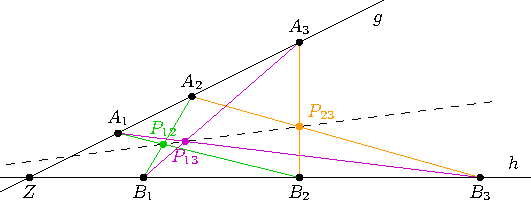
\includegraphics[width=12cm]{img/pappos}
\end{figure*}

\begin{thm}
 Sei $V$ ein $K$-Vektorraum über einem Schiefkörper $K$ und $\dim V \ge 3$. Dann gilt in $\proj(V)$ der Satz von Pappos genau dann, wenn $K$ kommutativ, also ein Körper ist.
\end{thm}

\begin{proof}
 Seien 
 \[ \begin{aligned}
     Z   &:= g \cap h = [u], \\
     A_1 &:= [v] \text{ und o.B.d.A. } A_2 = [u + v] \text{ (ersetze ggf. $v$ durch ein geeignetes $\lambda v$)}, \\
     B_1 &:= [w] \text{ und o.B.d.A. } B_2 = [u + w].
    \end{aligned} \]
 $u, v, w$ sind linear unabhängig, da $g \ne h$. Dann ist $P_{12} = A_1 B_2 \cap A_2 B_1 = [u + v + w]$. 
 
 ``$\Leftarrow$'' Sei $K$ ein Körper. Zu zeigen: $P_{12}, P_{13}, P_{23}$ sind kollinear.
 
 Für $A_3, B_3$ gibt es $r, s \in K$ mit $A_3 = [ru+v]$, $B_3 = [su+w]$. Dann ist 
 \[ P_{13} = A_3 B_1 \cap A_1 B_3 = [ru + v, w] \cap [v, su + w] = [rsu+sv+rw] =: [v_{13}], \]
 denn $s(ru+v) + rw = rsu + sv + rw = sv + r(su + w)$. Dabei gilt $rs = sr$, weil $K$ kommutativ ist.
 \[ P_{23} = A_2 B_3 \cap A_3 B_2 = [u+v, su + w] \cap [ru + v, u+w] \]
 und es gilt
 \[ \begin{aligned}
    (rs-1)u + (s-1)v + (r-1)w 
    &= (s-1) (u+v) + (r-1)(su +w) \\
    &= (s-1)(u+w) + (s-1)(ru+v),
    \end{aligned} \]
 also folgt
 \[ P_{23} = [ (rs-1)u + (s-1)v + (r-1)w ] =: [v_{23}]. \]
 Wir sehen nun $v_{13} - v_{23} = u + v + w$, also ist $P_{12} \in P_{13} P_{23}$ und damit sind die Punkte kollinear.
 
 ``$\Rightarrow$'' Gelte der Satz von Pappos. Zu zeigen: $K$ ist ein Körper, also $rs = sr$ für $r,s \in K$.
 
 Seien o.B.d.A.\footnote{Wir schließen 0 und 1 aus, da sie mit allen Elementen von $K$ kommutieren.} $r,s \in K \setminus \{ 0, 1 \}$, $A_3 := [ru+v]$, $B_3 := [su+v]$. Dann gibt es $x,y \in V$ mit $[x+y] = [u + v + w]$.
 
 Seien $P_{13} = [x]$, $P_{23} = [y]$, dann gibt es wegen des Satzes von Pappos $t_1, \ldots, t_8 \in K$, so dass
 \begin{align*}
    x &=   &   t_1 v + t_2 (su+w) &= t_3 w + t_4 (ru+v) \tag{1} \\
    y &=   &   t_5 (u+v) + t_6 (su+w) &= t_7 (u+w) + t_8 (ru+v) \tag{2} \\
  x+y &=   &   u+v+w &= t_1 v + t_2 (su+w) + t_5 (u+v) + t_6 (su+w) \tag{3}
 \end{align*}
 Weil $u,v,w$ linear unabhängig sind, folgt aus (3)
 \[ \left. \begin{aligned}
    w: \quad 1 &= t_2 + t_6 \\
    u: \quad 1 &= (t_2+t_6) s + t_5 = s + t_5 \\
    v: \quad 1 &= t_1 + t_5
    \end{aligned}
    \quad \right\} \Rightarrow 
    \begin{aligned}
     t_1 &= s, \\
     t_2 &= 1 - t_6, \\
     t_5 &= 1 - s. 
    \end{aligned} \]
 Zusammen mit (1) folgt
 \[ v: \quad t_4 = t_1 = s, \qquad u: \quad t_2 s = t_4 r, \qquad w: \quad t_2 = t_3. \]
 Mit $t_2 = 1 - t_6$ aus (3) gilt also
 \[ (1-t_6)s = t_2 s = t_4 r = sr \qRq t_6 s = s - sr \qRq t_6 = 1 - srs^{-1}. \tag{$\circ$} \]
 Zusammen mit (2) folgt
 \[ u: \quad t_5 + t_6s = t_7 + t_8 r, \qquad v: \quad t_8 = t_5, \qquad w: \quad t_7 = t_6. \]
 Nun setzen wir ($\circ$) und $t_5 = 1-s$ ein:
 \begin{align*}
     t_5 + t_6 s = t_6 + t_5 r \quad
     &\Rightarrow & (1-s) + (s-sr) &= (1 - srs^{-1}) + (1-s)r \\
     &\Rightarrow & -srs^{-1} + r &= 0 \\
     &\Rightarrow & srs^{-1} &= r \\
     &\Rightarrow & rs &= sr. \qedhere 
 \end{align*}
\end{proof}

\begin{bem}
 Aus dem Beweis des Satzes folgt in $\proj(V)$ ($V$ ist ein $K$-Vektorraum mit $\dim V \ge 3$): $K$ kommutativ $\Leftrightarrow$ Es existieren paarweise verschiedene $Z, A_1, A_2, B_1, B_2 \in \proj(V)$ mit $Z = A_1 A_2 \cap B_1 B_2$. Für alle $A_3$ auf $A_1 A_2$ mit $A_3 \ne A_1, A_2$ und $B_3$ auf $B_1 B_2$ mit $B_3 \ne B_1, B_2$ gilt: $P_{ij} = A_i B_j \cap A_j B_i$, $i \ne j$ sind kollinear.
 
 Das heißt im Satz von Pappos kann man $Z, A_1, A_2, B_1, B_2$ fest wählen.
\end{bem}

\begin{deno*}
 Der Vektor $x \ne 0$ aus $K^n$ heißt \emph{homogene Koordinaten} von $[x] \in \proj(V)$. Falls $x \in K^n$ mit $x_n \ne 0$, dann ist
 \[ \left[ \begin{pmatrix} x_1 \\ \vdots \\ x_{n-1} \\ x_n \end{pmatrix} \right] =
    \left[ \begin{pmatrix} x_n^{-1} x_1 \\ \vdots \\ x_n^{-1} x_{n-1} \\ 1 \end{pmatrix} \right]. \]
\end{deno*}

Für $V = \real^n$ ist
\[ [x] = \left[ \frac{x}{\|x\|} \right] = \left[ \frac{-x}{\|x\|} \right]. \]
Der projektive Raum $\proj(\real^n)$ kann daher mit der $S^{n-1} \subseteq \real^n$ nach Identifikation von Antipodenpaaren identifiziert werden.
 
$S^{n-1}$ ist die Einheitssphäre. $x \in S^{n-1}$ heißt $x \in \real^n$, $\| x \| = 1$. Wir betrachten also statt Geraden die äquivalenten (gegenüberliegenden) Punkte der Einheitssphäre $S^{n-1}_\pm$, das heißt $x \sim x' \Leftrightarrow x = x'$ oder $x = -x'$.

\subsection{Dualität für projektive Ebenen}
\begin{thm}
 Sei $\proj = (P,G,I)$ eine projektive Ebene. Dann ist auch $\proj^* := (G,P,I^{-1})$ mit $I^{-1} := \{ (g,p) : (p,g) \in I \}$ eine projektive Ebene.
\end{thm}

$\proj^*$ ist die zu $\proj$ \emph{duale Ebene}. Offensichtlich gilt $\proj^{**} = \proj$.

\begin{proof}
 Zu zeigen: $\proj^*$ erfüllt die Axiome der projektiven Ebene A1), A2'), A3) und A4) (siehe S. \pageref{def:proj}).
 \begin{enumerate}[\hspace{.5cm}A2)]
  \item[A1)] Durch je zwei (verschiedene) Punkte $p_1$, $p_2$ geht genau eine Gerade.
  \item[A2')] Je zwei Geraden schneiden sich.
  \item[A3)] Auf jeder Geraden liegen mindestens drei Punkte.
  \item[A4)] Es gibt mindestens zwei Geraden.
 \end{enumerate}
 
 Die zu einer Aussage über $(P,G,I)$ duale Aussage ist die entsprechende Aussage für $(G,P,I^{-1})$\footnotemark.
 \footnotetext{Vertausche die Rollen von Punkten und Geraden und $I$ mit $I^{-1}$. Begriffe werden analog dualisiert, zum Beispiel die Gerade $P_1 P_2$ entspricht dem Punkt $g_1 \cap g_2$. Kollineare Punkte entsprechen kopunktalen Geraden.}
 
 Aus A1) und A2') folgt die Aussage:
 \begin{enumerate}[\hspace{.5cm}A2)]
  \item [$\widetilde{\text{A2}}$')] Je zwei Geraden schneiden sich in genau einem Punkt.
 \end{enumerate}

 Für die ersten beiden dualen Axiome folgt:
 \begin{enumerate}[\hspace{.5cm}{A}1 {dual})]
  \item[A1 dual)] ist offenbar dieselbe Aussage wie $\widetilde{\text{A2}}$').
  \item[A2' dual)] ist dieselbe Aussage wie A1).
 \end{enumerate}

 Die zu A3) und A4) dualen Aussagen sind
 \begin{enumerate}[\hspace{.5cm}{A}1 {dual})]
  \item[A3 dual)] Durch jeden Punkt gehen mindestens drei Geraden.
  \item[A4 dual)] Es gibt mindestens zwei Punkte.
 \end{enumerate}
 Aus A3) und A4) folgt offenbar A4 dual). 
 
 Zu zeigen: In $\proj$ gilt A3 dual). Sei $P$ ein Punkt. Dann gibt es nach A1) eine Gerade $g$ durch $P$.  Auf dieser liegen nach A3) mindestens zwei weitere Punkte $P_1$ und $P_2$. Nach A4) gibt es mindestens eine weitere Gerade $h$ und nach A2') schneiden sich $g$ und $h$ in einem Punkt $X$. Auf $h$ gibt es nach A3) zwei Punkte $Q_1, Q_2 \ne X$. Die Geraden $PQ_1, PQ_2$ und $PP_1$ sind paarweise verschieden. Damit gibt es mindestens drei Geraden durch $P$.
\end{proof}

\textbf{Dualitätsprinzip.} Wenn eine Aussage für alle projektiven Ebenen gilt, dann gilt auch die duale Aussage für alle projektiven Ebenen\footnote{Vertausche zum Beweis einfach $\proj$ mit $\proj^*$.}.

\begin{exmp*}
 Dualisiere die Aussage ``$\proj = (P,G,I)$ ist desarguessch.'' Beweise: Wenn $\proj$ desarguessch ist, dann ist es auch $\proj^*$.
 
 \begin{addmargin}[.5cm]{0cm} 
 \textbf{Aussage von Desargues.} Für alle $A_1, A_2, A_3, B_1, B_2, B_3 \in P$ mit $A_i \ne B_i$, sodass $A_1, A_2, A_3$ nicht kollinear sind und $B_1, B_2, B_3$ nicht kollinear sind, gilt: Falls $Z$ der Schnittpunkt von $A_1 B_1$, $A_2 B_2$ und $A_3 B_3$ ist, dann sind 
 \begin{align*}
  P_{12} &:= A_1 A_2 \cap B_1 B_2, \\
  P_{23} &:= A_2 A_3 \cap B_1 B_2, \\
  P_{13} &:= A_3 A_1 \cap B_3 B_1 
 \end{align*}
 kollinear.
 
 \textbf{Duale Aussage.} Für alle $g_1, g_2, g_3, h_1, h_2, h_3 \in G$ mit $g_i \ne h_i$, sodass $g_1, g_2, g_3$ nicht kopunktal\footnote{Das heißt, dass die drei Geraden sich nicht in \emph{einem} Punkt schneiden, sondern ein Dreieck bilden.} und $h_1, h_2, h_3$ nicht kopunktal sind, gilt: Falls $f$ eine Gerade durch $g_1 \cap h_1$, $g_2 \cap h_2$, $g_3 \cap h_3$ ist, dann sind
 \begin{align*}
  l_{12} &:= (g_1 \cap g_2)(h_1 \cap h_2), \\
  l_{23} &:= (g_2 \cap g_3)(h_2 \cap h_3), \\
  l_{31} &:= (g_3 \cap g_1)(h_3 \cap h_1 )
 \end{align*}
 kopunktal.
 \end{addmargin}
\end{exmp*}

\setcounter{thm}{5}
\begin{thm}
 Eine projektive Ebene $\proj$ ist desarguessch $\Leftrightarrow$ $\proj^*$ ist desarguessch.
\end{thm}

\subsection{Endliche projektive Räume}

\begin{defn*}
 Ein projektiver Raum $\proj = (P,G,I)$ heißt \emph{endlich}, falls $P$ endlich ist.
\end{defn*}

\begin{deno*}
 Sei $g \in G$, dann bezeichnet $(g) := \{ p \in P : (p,g) \in I \}$ die Menge der Punkte auf der Geraden $g$.
\end{deno*}

\begin{thm*}[Hessenberg]
 Sei $\proj$ ein projektiver Raum, in dem der Satz von Pappos gilt. Dann gilt auch der Satz von Desargues.
\end{thm*}

Beweis nicht in der Vorlesung, siehe zum Beispiel
\begin{itemize}
 \item H. Lenz: Vorlesungen über projektive Geometrie,
 \item R. Lingenberg: Grundlagen der Geometrie I.
\end{itemize}

Beispiel für eine nichtdesarguessche projektive Ebene (siehe auch Übung): Moulton-Ebene.

\begin{lem}
 Sei $\proj$ ein projektiver Raum, $g_1, g_2 \in G$. Dann gibt es eine bijektive Abbildung $\varphi:(g_1) \to (g_2)$.
\end{lem}

\begin{proof}
 Sei O.B.d.A. $g_1 \ne g_2$. Wir unterscheiden zwei Fälle:
 \begin{enumerate}
  \item $(g_1) \cap (g_2) = \{ s \} \ne \emptyset$. Seien $P_1 \in (g_1)$, $P_2 \in (g_2)$ mit $P_1 \ne P_2 \ne S$ (diese existieren nach A3)). Nach A3) gibt es auch $P$ mit $P \ne P_1$, $P \ne P_2$ auf $P_1 P_2$. Es ist offenbar $P \notin (g_1)$ und $P \notin (g_2)$. Nach A2) schneidet eine Gerade $Px$ mit $x \in (g_1)$, $x \ne S$ die Gerade $g_2$ in einem eindeutig bestimmten Punkt $\pi(x) \ne S$. Die Gerade $PS$ schneidet $g_2$ nur in $S$. Definiere $pi:(g_1) \to (g_2)$ mit $\pi( x ) = xP \cap g_2$. $\pi$ ist offenbar bijektiv.
  \item $(g_1) \cap (g_2) ) \emptyset$. Wähle  auf $g_1$, $g_2$ Punkte $P_1 \in (g_1)$, $P_2 \in (g_2)$. Sei $h := P_1 P_2$. Dann gibt es nach dem 1. Fall bijektive Abbildungen $\pi_1: (g_1) \to (h)$ und $\pi_2: (h) \to (g_2)$. Also ist $\pi_2 \circ \pi_1: (g_1) \to (g_2)$ bijektiv. \qedhere
 \end{enumerate}
\end{proof}

\begin{figure*}[ht]
 \center
 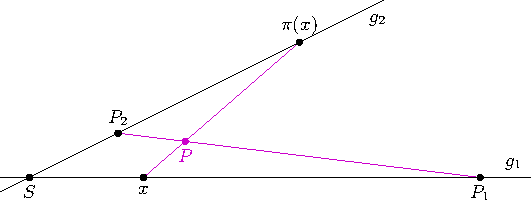
\includegraphics[width=12cm]{img/lemma27}
\end{figure*}

In einem endlichen projektiven Raum $\proj$ liegen also auf jeder Geraden gleich viele Punkte.

\begin{defn*}
 Ein endlicher projektiver Raum $\proj$ hat die \emph{Ordnung $q$}, wenn auf jeder Geraden $q+1$ Punkte liegen.
\end{defn*}

\begin{thm*}[Wedderburn]
 Jeder endliche Schiefkörper ist ein Körper.
\end{thm*}

\begin{thm}
 Sei $\proj = (P,G,I)$ eine projektive Ebene der Ordnung $q$. Dann gilt $|P| = |Q| = q^2 + q +1$. Auf jeder Geraden liegen $q+1$ Punkte und durch jeden Punkt gehen $q+1$ Geraden.
\end{thm}

\begin{proof}
 Nach Lemma 2.7 und Definition liegen auf jeder Geraden genau $q+1$ Punkte. Sei $p \in P$, $g \in G$ mit $p \notin (g)$. Jede Gerade durch $p$ schneidet $(g)$ in genau einem Punkt und durch jeden Punkt $p_1 \in (g)$ gibt es die Gerade $p p_1$. Damit haben wir eine Bijektion zwischen der Menge der Geraden durch $p$ und der Menge der Punkte auf $g$ definiert. Also gehen durch jeden Punkt $p$ genau $q++1$ Geraden. Damit gibt es genau 
 \[ \text{(Geraden durch $p$)} \cdot \text{(Punkte $\ne p$ auf $g$ durch $p$)} + \text{Punkt $p$} = (q+1)q + 1 = q^2 + q +1 \]
 Punkte. Dies ist auch gleich der Anzahl der Geraden, da $\proj^* = (G,P,I^{-1})$ auch eine projektive Ebene der Ordnung $q$ ist.
\end{proof}

\subsubsection*{Endliche Körper}
\begin{defn*}
 Sei $K$ ein Körper. Die \emph{Charakteristik} von $K$ ist definiert als
 \[ \chr K = \begin{cases} 
    p, &\text{falls $p \in \nat$ die kleinste Zahl mit $1 + 1 + \ldots + 1 = 0$ ist.} \\
    0, &\text{falls es keine solche Zahl gibt.}         
   \end{cases} \]
Falls $\chr K \ne 0$, dann ist $\chr K$ eine Primzahl, denn anderenfalls wäre $p = nm$ mit $1 < n < p$ und $1 < m < p$, also
\[ \underbrace{( 1 + 1 + \ldots + 1)}_n \cdot \underbrace{( 1 + 1 + \ldots + 1)}_m = 0 \]
\end{defn*}

\begin{exmp*}
 $\integer_p$ ist für eine Primzahl $p$ ein Körper der Charakteristik $p$.  
\end{exmp*}

Falls $K$ ein endlicher Körper ist, dann ist $\chr(K) = p \ne 0$ eine Primzahl. In $K$ betrachte die Menge
\[ P := \{ 0, 1, 1+1, \ldots, (p-1) \cdot 1 \} \subseteq K. \]
Dies ist ein Unterkörper von $K$ und $K$ ist ein $P$-Vektorraum, $\dim K = n \ne \infty$. $K$ hat genau $p^n$ Elemente. Also ist $(K,+) \simeq \integer_p^n$.

Es gilt $(K \setminus \{ 0 \}, \cdot ) \simeq \integer_{q-1}$, wobei $q = p^n = |K|$, das heißt es gibt $a \in K$ mit
\[ K^* := K \setminus \{ 0 \} = \{ 1, a, a^2, a^3, \ldots, a^{q-2} \}. \]
Also ist jedes Element von $K$ Nullstelle des Polynoms $x^q - x \in K[x]$. 

Die Abbildung $\varphi: K \to K$ mit $\varphi(x) = x^p$ ist ein Körperautomorphismus von $K$, denn
\begin{align*}
 \varphi(xy) &= (xy)^p = \varphi(x) \varphi(y) \\
 \varphi(x+y) &= (x+y)^p = \sum_{\nu = 0}^p \begin{pmatrix} p \\ \nu \end{pmatrix} x^\nu y^{p-\nu} \overset{\footnotemark}{=} x^p + y^p = \varphi(x) + \varphi(y)
\end{align*}
\footnotetext{Denn $\begin{pmatrix} p \\ \nu \end{pmatrix}$ ist  in $K$ für $1 \le \nu \le p-1$ durch $p$ teilbar, also $\begin{pmatrix} p \\ \nu \end{pmatrix} = 0$.}

$\varphi$ ist bijektiv, denn $\varphi^n = \id$,  $x^{p^n} = x^q = x$.

\begin{thm*}
 Sei $p$ eine Primzahl und $n \in \nat$. Dann gibt es bis auf Isomorphie genau einen Körper mit $q=p^n$ Elementen. Er ist der ``kleinste'' Körper, in dem das Polynom $x^q - x \in P[x]$ in Linearfaktoren zerfällt\footnote{Der ``Zerfällungskörper'' von $x^q - x$ über $P$.}.
 
 Die Unterkörper von $K$ mit $q = p^n$ sind genau die Körper der Form 
 \[ \{ x \in K | x^{p^i} = x \} = \{ 0 \} \cup \{ a^{k p^{n-i}} : k = 0, 1, \ldots, p^i -1 \},\]
 wobei $i \ge 1$ ein Teiler von $n$ ist. Also gibt es zu jedem $i \ge 1$ mit $i|n$ ($i$ teilt $n$) genau einen Unterkörper von $K$ mit $p^n$ Elementen und diese sind alle Unterkörper von $K$.
\end{thm*}

\subsubsection*{Konstruktion eines Körpers mit \texorpdfstring{$p^n$}{p hoch n} Elementen}
Wähle ein irreduzibles\footnote{Irreduzibel heißt, dass es \emph{keine} Polynome $p_1, p_2$ kleineren Grades gibt, sodass $p_0 = p_1 p_2$.} Polynom $n$-ten Grades $p_0(x) \in \integer_p[x]$. Dann ist $\integer_p[x] / (p_0)$ ein Körper mit $p^n$ Elementen.

Erzeugtes Ideal
\[ \{ p_0 f | f \in \integer_p[x] \} \]

\begin{defn*}\label{def:kollineation}
 Sei $\proj = (P,G,I)$, $\proj' = (P',G',I')$ projektive Räume. Eine \emph{Kollineation} $\alpha: \proj \to \proj'$ ist ein Paar $\alpha = (\alpha_1, \alpha_2)$ von bijektiven Abbildungen $\alpha_1:P \to P'$, $\alpha_2: G \to G'$, sodass $(p,g) \in I \Leftrightarrow (\alpha_1(p), \alpha_2(g) ) \in I'$ für alle $p \in P$, $g \in G$. 
 
 $\proj=(P,G,I)$ und $\proj' = (P', G', I')$ heißen \emph{isomorph} (geschrieben $\proj \simeq \proj'$), wenn es eine Kollineation $\alpha: \proj \to \proj'$ gibt.
 
 Schreibweise: Wir schreiben $\alpha(p), \alpha(g)$ statt $\alpha_1(p), \alpha_2(g)$, falls keine Missverständnisse zu befürchten sind.
\end{defn*}

\begin{bem}
 Die Menge der Kollineationen $\alpha: \proj \to \proj'$ ist mit $\circ$ eine Gruppe.
\end{bem}

\begin{thm*}[Koordinatisierungssatz]
 Sei $\proj = (P,G,I)$ ein desarguesscher projektiver Raum. Dann gibt es einen Schiefkörper $K$ mit einem $K$-Vektorraum $V$ mit $\dim V \ge 3$, sodass $\proj \simeq \proj(V)$ gilt.
\end{thm*}

\subsubsection*{Desarguessche endliche projektive Ebenen}
Sei $\proj$ eine endliche desarguessche projektive Ebene. Nach dem Koordinatisierungssatz gibt es einen $K$-Vektorraum $V$ über einem Schiefkörper $K$ mit $\proj \simeq \proj(V)$ und $\dim V \ge 3$. Da $\proj$ endlich ist, ist auch $K$ endlich. Nach dem Satz von Wedderburn ist $K$ ein Körper. Also hat $K$ nach Klassifikation der endlichen Körper $p^n$ Elemente, wobei $p$ eine Primzahl ist.

Ferner gilt: Bis auf Isomorphie gibt es zu jeder Primzahl $p$ und $n \in \nat$ genau einen solchen Körper mit $q = p^n$ Elementen. Man bezeichnet ihn mit $GF(q)$ bzw. $\mathbf{F}_q$.

Bis auf Isomorphie gibt es genau eine desarguessche projektive Ebene der Ordnung $q = p^n$.

\subsubsection*{Nichtdesarguessche endliche projektive Ebenen}
Für jedes $q \le 8$ gibt es \emph{keine} nichtdesarguessche projektive Ebene der Ordnung $q$. Für jedes $q = p^n$ mit $n \ge 2$, $p$ Primzahl, $q \ge 9$ gibt es (mindestens) eine nichtdesarguessche projektive Ebene der Ordnung $q$.

\emph{Jede bisher bekannte} endliche projektive Ebene ist von der Ordnung $q = p^n$, $p$ Primzahl, $n \ge 1$. \emph{Jede bisher bekannte} projektive Ebene von Primzahlordnung ist desarguessch.

\textbf{Folgerung aus Koordinatisierungssatz, Satz von Wedderburn und Satz von Hessenberg.}
In einer endlichen projektiven Ebene $\proj$ sind äquivalent:
\begin{enumerate}[(1)]
 \item $\proj$ ist desarguessch.
 \item In $\proj$ gilt der Satz von Pappos.
\end{enumerate}

Ein Satz zur Nicht-Existenz bestimmter projektiver Ebenen:
\begin{thm*}[Bruck-Ryser]
 Falls $q = 4n+1$ oder $q = 4n+2$, $n \in \nat$ \emph{und} $q$ nicht die Summe zweier Quadratzahlen ist, dann gibt es \emph{keine} projektive Ebene der Ordnung $q$.
\end{thm*}

\begin{bem}
 Sei $q = r^2 m$, $r,m \in \nat$ und $m$ nicht durch eine Quadratzahl teilbar, dann sind äquivalent:
 \begin{enumerate}[(1)]
  \item $q$ ist \emph{nicht} die Summe zweier Quadratzahlen.
  \item $m$ ist durch eine Zahl der Form $4k+3$ teilbar, $k \in \nat_0$.
 \end{enumerate}
\end{bem}

Das Wissen um die Nichtexistenz von projektiven Ebenen anderer Ordnung als im Satz von Bruck-Ryser ist sehr begrenzt. Die einzige andere Zahl, die bisher als Ordnung einer projektiven Ebene ausgeschlossen wurde, ist $q = 10$. Dieser Beweis wurde mit massivem Computereinsatz geführt.

Also sind bisher bekannt:
\begin{center}\begin{tabular}{l|c|c|c|c|c|c|c|c|c|c}
 Ordnung &    & 2  & 3  & 4  & 5  & 6    & 7  & 8  & 9  & 10 \\
 \hline
 Bekannt &    & Ja & Ja & Ja & Ja & Nein & Ja & Ja & Ja & Nein* \\[5pt]
 Ordnung & 11 & 12 & 13 & 14 & 15 & 16 & 17 & 18 & 19 & 20 \\
 \hline
 Bekannt & Ja & ?  & Ja & Nein & ? & Ja & Ja & ? & Ja & ?
\end{tabular}\end{center}

\subsection{Unterräume projektiver Räume}
\begin{defn*}
 Sei $\proj = (P,G,I)$ ein projektiver Raum. $U \subseteq P$ heißt ein \emph{Unterraum}, falls für je zwei (verschiedene) Punkte $p_1, p_2 \in U$ gilt $(p_1 p_2) \subseteq U$.
\end{defn*}

Offensichtlich erfüllt für jeden Unterraum $U \subseteq P$ die Inzidenzstruktur $\ubar{U} = (U,G',I')$ mit $G' = \{ g \in G : (g) \subseteq U \}$ die Axiome A1), A2), A3), aber \emph{nicht unbedingt} A4).

Also nach Definition sind $\emptyset$, $\{ p \}$, $(g)$ für $p \in P$, $g \in G$ Unterräume von $\proj$, aber keine projektiven Räume, da A4) nicht erfüllt ist. 

Der Durchschnitt beliebiger Unterräume ist wieder ein Unterraum.

\begin{defn*}
 Sei $X \subseteq P$. Dann definiere $\angles{x} := \bigcap \{ U : x \in U, U \subset P \text{ Unterraum} \}$. $\angles{x}$ heißt der von $x$ \emph{aufgespannte Unterraum}. Er ist der kleinste Unterraum von $\proj$, der $x$ enthält.
 
 $x$ heißt ein \emph{Erzeugendensystem} in $\proj$, falls $\angles{x} = P$.
 
 $\proj$ heißt \emph{endlich erzeugbar}, falls es ein endliches Erzeugendensystem gibt.
 
 Schreibweisen: Statt $\angles{ \{p_1, \ldots, p_n \} }$ schreibe $\angles{ p_1, \ldots, p_n }$. Statt $\angles{ x \cup \{p\} }$ schreibe $\angles{x,p}$. Statt $\angles{x \cup y}$ schreibe $\angles{x,y}$.
 
 $\angles{ \emptyset } = \emptyset$, $\angles{ p } = \{ p \}$ für $p \in P$, $\angles{ p,q } = ( pq )$, falls $p \ne q$, $p,q \in P$
\end{defn*}

\setcounter{thm}{17}
\begin{prp}
 Sei $U \subseteq P$ ein Unterraum, $p \in P \setminus U$, $U \ne \emptyset$. Dann gilt
 \[ \angles{ U,p } = \bigcup \{ (pq) : q \in U \}. \]
\end{prp}

Beweis als Übung, das Axiom A2) wird dabei wesentlich verwendet.

\begin{prp}[Austauschsatz]
 Sei $U \subseteq P$ ein Unterraum, $U \ne \emptyset$ und $p \in P \setminus U$. Dann gilt: Aus $q \in \angles{U,p} \setminus U$ folgt $p \in \angles{U,q}$.
\end{prp}

\begin{proof}
 Wegen $q \in \angles{U,p} \setminus U$ gibt es nach 2.18 einen Punkt $q' \in P$ mit $q \in \angles{p,q'}$. Es gilt $p \notin U$, $q \notin U$, $q' \in U$, also $p \ne q'$ und $q \ne q'$ und damit $p \in \angles{q,q'}$.  Daraus folgt $p \in \angles{U,q}$, also $\angles{U,p} \subset \angles{U,q}$.
 
 Andererseits ist $\angles{U,q} \subset \angles{U,p}$ wegen $q \in \angles{U,p}$.
\end{proof}

\subsection{Basisergänzungssatz}
\begin{defn*}
 Eine Menge $B \subseteq P$ heißt \emph{unabhängig}, falls für alle $p \in B$ gilt $p \notin \angles{ B \setminus \{ p\}}$. Eine unabhängige Menge $B \subseteq P$ mit $\angles{B} = P$ heißt \emph{Basis} von $P$.
\end{defn*}

\begin{prp}
 Eine Menge $B \subseteq P$ ist genau dann eine Basis von $P$, wenn $B$ ein minimales Erzeugendensystem ist.
\end{prp}

\begin{proof}
 Klar.
\end{proof}

\begin{prp}
 Sei $E \subseteq P$ ein endliches Erzeugendensystem. Dann gibt es eine Basis $B \subseteq E$.
\end{prp}

\begin{proof}
 Sei $E_0 := E$. Falls $E_0$ unabhängig ist, dann ist es eine Basis. Anderenfalls $p_0 \in E_0$ mit $p_0 \in \angles{E_0 \setminus \{ p_0 \}}$. Definiere $E_1 := E_0 \setminus \{ p_0 \}$ und beginne von vorn. Da $E$ endlich ist, erhält man nach endlich vielen Schritten eine Basis.
\end{proof}

\begin{rmrk*}
 Bei einem unendlichen Erzeugendensystem kann man nicht so vorgehen, sondern man muss mit Hilfe des Zornschen Lemmas die Existenz einer maximalen unabhängigen Menge $B \subseteq E$ nachweisen und dann, dass eine solche maximale unabhängige Menge ein Erzeugendensystem ist\footnote{Der Beweis, dass jeder Vektorraum eine Basis hat, ist analog.}. Für das Zornsche Lemma braucht man das Auswahlaxiom.
\end{rmrk*}

\clearpage

\begin{lem}
 Sei $B \subseteq P$ eine unabhängige Menge, $B$ endlich. Seien $B_1 \subseteq B_2$, $B_2 \subseteq B$. Dann gilt
 \[ \angles{ B_1 \cap B_2 } = \angles{B_1} \cap \angles{B_2}. \]
\end{lem}

\begin{proof}
 Einfache Übung.
\end{proof}

\begin{thm}[Steinscher Austauschsatz]
 Sei $B$ eine endliche Basis von $P$ und sei $C \subseteq P$ unabhängig. Dann gilt
 \begin{enumerate}[a)]
  \item $|C| \le |B|$,
  \item es gibt eine Teilmenge $\tilde{B} \subseteq B$ mit $|\tilde{B}| = |B| - |C|$, so dass $C \cup \tilde{B}$ eine Basis von $P$ ist.
 \end{enumerate}
\end{thm}

\begin{proof}
 Einfache Übung.
\end{proof}

\textbf{Folgerung:}
\begin{thm}[Basisergänzungssatz]
 Sei $\proj$ ein endlich erzeugbarer projektiver Raum. Dann haben je zwei Basen von $P$ dieselbe Anzahl von Elementen und jede unabhängige Teilmenge von $P$ lässt sich zu einer Basis ergänzen.
\end{thm}

\begin{proof}
 Nach Proposition 2.21 hat $P$ eine endliche Basis $B$. Sei $r := |B|$. Nach Satz 2.23 hat jede unabhängige Menge, also auch jede Basis höchstens $r$ Elemente. Falls $B_1$, $B_2$ zwei Basen sind, folgt aus 2.23 a) $|B_1| \le |B_2|$ und $|B_2| \le |B_1|$, also $|B_2| = |B_1|$.
 
 Sei $C$ eine unabhängige Menge, dann lässt sie sich nach 2.23 b) zu einer Basis ergänzen.
\end{proof}

\subsection{Dimensionssatz}
\begin{defn*}
 Sei $\proj$ ein projektiver Raum. Falls $P$ eine Basis mit $d+1$ Elementen hat, so heißt $\proj$ \emph{$d$-dimensional}. Schreibweise $\dim \proj = d$. Entsprechend $\dim \uproj = d$, falls es eine Basis von $U$ mit $d+1$ Elementen gibt, wobei $U \subseteq P$ ein Untervektorraum sei. Also
 \begin{itemize}
  \item $\dim \emptyset = -1$,
  \item $\dim \{ p \} = 0$ für alle $p \in P$,
  \item $\dim (p_1 p_2) = 1$ für $p_1 \ne p_2$,
  \item $\dim \proj = 2$ für die projektive Ebene.
 \end{itemize}
 $\dim \proj = \infty$, falls $P$ kein endliches Erzeugendensystem besitzt.
\end{defn*}

\begin{defn*}
 Eine \emph{Hyperebene} $H \subseteq P$ ist ein Unterraum, so dass $H \ne P$ gilt und es $p \in P \setminus H$ gibt, so dass $P = \angles{ H, p }$.
 
 Offenbar gilt: Falls $\dim P = d < \infty$ und $H$ ein Unterraum ist, dann ist $H$ eine Hyperebene $\Leftrightarrow$ $\dim H = d-1$.
\end{defn*}

\begin{thm}[Dimensionssatz]
 Sei $P$ endlich-dimensional. Seien $U, W \subseteq P$ Unterräume. Dann gilt
 \[ \dim \angles{U,W} = \dim U + \dim W - \dim (U \cap W). \]
\end{thm}

\begin{proof}
 Übung.
\end{proof}

\subsection{Desarguessche projektive Räume}
\begin{thm}
 Jeder projektive Raum $\proj$ der Dimension $\dim \proj \ge 3$ ist desarguessch.
\end{thm}

\begin{proof}
 Seien $a_1, a_2, a_3$, $b_1, b_2, b_3$, $z$ Punkte, die die Voraussetzungen des Satzes von Desargues erfüllen, also zum Beispiel $z = (a_1 b_1) \cap (a_2 b_2) \cap (a_3 b_3)$.
 
 1. Fall: Die Ebenen $\pi = \angles{a_1, a_2, a_3}$ und $\psi = \angles{b_1, b_2, b_3}$ sind verschieden. Da $b_i \in (a_i z)$ folgt, dass $b_1, b_2, b_3 \in U := \angles{z, a_1, a_2, a_3}$. Ferner schneiden sich $(a_i a_j)$ und $(b_i b_j)$, da beide Geraden in der gemeinsamen Ebene $\angles{z, a_i, a_j} = \angles{ z, a_i, a_j, b_i, b_j}$ liegen.
 
 Sei $p_{ij} = (a_i a_j) \cap (b_i b_j)$. Die Punkte $p_{12}, p_{23}, p_{13}$ liegen in $\pi \cap \psi$. Da sich zwei verschiedene Ebenen von $U$ in genau einer Geraden schneiden, sind $p_{12}, p_{23}, p_{13}$ kollinear.
 
 2. Fall: Die Punkte $a_1, a_2, a_3$, $b_1, b_2, b_3$ und damit $z$ liegen in einer gemeinsamen Ebene $\pi$. Dann wähle $z' \in P \setminus \pi$ (dieser existiert, da $\dim \proj \ge 3$) und einen dritten Punkt $z'' \in (zz')$. Wegen $z \in (z'z'') \cap (a_1 b_1)$ spannen $z'z''$ und $a_1 b_1$ eine Ebene auf, also schneiden sich $z'a_1$ und $z'' b_1$  in einem Punkt $c_1 \notin \pi$ (da $a_1 \in \pi$ würde aus $c_1 \in \pi$ folgen $z' \in \pi$, Widerspruch). Entsprechend existieren $c_2, c_3 \notin \pi$ mit $c_2 := z' a_2 \cap z'' b_2$ und $c_3 := z' a_3 \cap z'' b_3$.
 
 $c_1, c_2, c_3$ sind nicht kollinear, denn anderenfalls wäre $\dim \angles{c_1,c_2,c_3,z'} \le 2$. Wegen $a_i \in (z' c_i)$ wären die $a_i \in \pi \cap \angles{c_1, c_2, c_3, z'}$. Der Durchschnitt hätte $\dim \le 1$, also wäre die $a_i$ kollinear. Widerspruch!
 
 Sei nun $\psi := \angles{c_1,c_2,c_3}$. Nach dem 1. Fall schneiden sich $c_i c_j$ und $a_i a_j$ und es gilt $c_1 c_2 \cap a_1 a_2$, $c_2 c_3 \cap a_2 a_3$, $c_1 c_3 \cap a_1 a_3 \in g := \pi \cap \psi$. Nun gilt also $c_i c_j \cap a_i a_j \in g$ und $c_i c_j \cap b_i b_j \in g$, es folgt $c_i c_j \cap a_i a_j = c_i c_j \cap g = c_i c_i \cap b_i b_j$. 

 Definiere $a_i a_j \cap b_i b_j =: P_{ij}$. Die $P_{ij}$ liegen auf der Geraden $g$.
\end{proof}

\begin{folg*}
 Eine projektive Ebene, die isomorph zu einem Unterraum in einem höher\-dimen\-sionalen Raum ist, ist desarguessch.
\end{folg*}

\clearpage
\setcounter{secnumdepth}{1}
\section{Die Struktursätze und Zentralkollineationen}
\setcounter{secnumdepth}{0}

\begin{thm}[Koordinatierungssatz, 1. Hauptsatz der projektiven Geometrie]
 Sei $\proj$ ein desarguesscher projektiver Raum. Dann gibt es einen Schiefkörper $K$, einen $K$-Vektorraum $V$ und eine Kollineation\footnotemark $\alpha: \proj \to \proj(V)$ (das heißt $\proj \simeq \proj(V)$). 
\end{thm}
\footnotetext{Def. siehe Seite \pageref{def:kollineation}.}

Der Beweis des Satzes ist sehr lang und wird daher weggelassen.

\subsection{Darstellung von Kollineationen durch bijektive semilineare Abbildungen}
\begin{defn*}
 Seien $V, V'$ Vektorräume über $K$ bzw. $K'$ (Schiefkörper). Eine \emph{semilineare Abbildung} $\varphi: V \to V'$ bezüglich eines Körperisomorphismus $\alpha: K \to K'$ ist eine Abbildung, sodass für alle $x,y \in V$ gilt
 \[ \varphi(x+y) = \varphi(x) + \varphi(y) \]
 und für alle $x \in V$, $\lambda \in K$ gilt
 \[ \varphi( \lambda x ) = \alpha(\lambda) \varphi(x). \]
\end{defn*}

\begin{exmp*}
 $\varphi: \complex^3 \to \complex^3$ mit
 \[ \varphi\left( \begin{pmatrix} x_1 \\ x_2 \\ x_3 \end{pmatrix} \right) = \begin{pmatrix} \obar{x_1} \\ \obar{x_2} \\ \obar{x_3} \end{pmatrix} \]
 ist eine semilineare Abbildung bezüglich der komplexen Konjugation.
 \[ \varphi\left( \lambda \begin{pmatrix} x_1 \\ x_2 \\ x_3 \end{pmatrix} \right) = \obar{\lambda} \begin{pmatrix} \obar{x_1} \\ \obar{x_2} \\ \obar{x_3} \end{pmatrix} = \obar{\lambda} \varphi\left( \lambda \begin{pmatrix} x_1 \\ x_2 \\ x_3 \end{pmatrix} \right). \]
\end{exmp*}

\begin{thm}
 Seien $V, V'$ Vektorräume über Schiefkörpern $K$ bzw. $K'$ mt $\dim V = \dim V' \ge 3$. Sei $\varphi : V \to V'$ semilinear bezüglich eines Körperisomorphismus $\alpha: K \to K'$ und bijektiv, dann
 \begin{enumerate}[a)]
  \item $\obar{\varphi} : \proj(V) \to \proj(V')$ mit $\obar{\varphi}( [x] ) := [\varphi(x)]$ ist eine Kollineation\footnotemark, wenn $x, y$ linear unabhängig sind.
  \item Falls $\varphi': V \to V'$ ebenfalls semilinear bezüglich $\alpha': K \to K'$ und bijektiv ist mit $\obar{\varphi}' = \obar{\varphi}$, dann gibt es genau ein $b \in K' \setminus \{ 0 \}$, sodass $\varphi'(x) = b \cdot \varphi(x)$ für alle $x \in K$ und $\alpha'(\lambda) = b \alpha(\lambda) b^{-1}$.
 \end{enumerate}
\end{thm}
\footnotetext{Das heißt $\obar{\varphi}([x,y]) = [ \varphi(x), \varphi(y)]$.}

\begin{proof}
 \begin{enumerate}[a)]
  \item $\obar{\varphi}$ ist wohldefiniert:
   \[ \obar{\varphi}( [\lambda x] ) = [\alpha(\lambda) \varphi(x) ] = [\varphi(x)] \]
   für $\lambda \in K \setminus \{0\}$.
   \[ \begin{aligned}
      \varphi(Kx + Ky )
      &= \{ \varphi( \lambda x + \mu y) : \lambda, \mu \in K \} \\
      &= \{ \alpha( \lambda ) \varphi(x) + \alpha( \mu ) \varphi(y) \} \\
      &= K' \varphi(x)  + K' \varphi(y),
      \end{aligned} \]
   $\obar{\varphi}$ bildet also Geraden in $\proj(V)$ auf Geraden in $\proj(V')$ ab.
  \item Eindeutigkeit bis auf Vielfache: $\eta := \varphi^{-1} \circ \varphi_ V \to V$ ist eine bijektive semilineare Abbildung, bei der jeder Vektor auf ein Vielfaches ($\ne 0$) abgebildet wird.
  
  Seien $x,y$ linear unabhängig. Dann folgt, dass es $\lambda_1, \lambda_2, \lambda_3 \in K \setminus \{ 0 \}$ gibt mit
  \[ \eta(x) = \lambda_1 x, \quad \eta(y) = \lambda_2 y, \quad \eta(x+y) = \lambda_3 (x+y)  = \eta(x) + \eta(y) = \lambda_1 x + \lambda_2 y, \]
  also $\lambda_1 = \lambda_2 = \lambda_3$. Damit ist der Faktor für linear unabhängige Vektoren derselbe. Somit haben wir für alle $x,y \in V$ denselben Faktor, das zu $x,y$ einen linear unabhängigen Vektor $z$ gibt. Der Faktor $b$ ist eindeutig bestimmt, da für $x \ne 0$ gilt
  \[ \eta(x) = bx = b'x \qRq b = b'. \]
  Also ist $\eta = b \cdot \id$ und damit folgt $\varphi' = b \cdot \varphi$.
  
  Ferner ist
  \[ \varphi( \lambda x ) = \alpha'(\lambda) \varphi'(x) = \alpha'(\lambda) b \varphi(x) \]
  und
  \[ b \varphi(\lambda x) = b \alpha(\lambda) \varphi(x), \]
  daraus folgt für $x \ne 0$
  \[ \alpha'(\lambda) = b \alpha( \lambda ) b^{-1}. \qedhere \]
 \end{enumerate}
\end{proof}

$\obar{\varphi}$ injektiv: Falls $[x] \ne [y]$, also $x$ und $y$ linear unabhängig, folgt wegen der Bijektivität und Semilinearität von $\varphi$, dass $\varphi(x)$ und $\varphi(y)$ linear unabhängig sind. Damit gilt $[\varphi(x)] \ne [\varphi(y)]$.

\begin{rmrk*}
 Falls $\varphi_1 : V \to V'$ semilinear bezüglich $\alpha_1$ und $\varphi_2: V' \to V''$ semilinear bezüglich $\alpha_2$ ist, dann ist $\varphi_2 \circ \varphi_1: V \to V''$ semilinear bezüglich $\alpha_2 \circ \alpha_1$.
\end{rmrk*}

\begin{thm}[2. Hauptsatz der projektiven Geometrie]
 \textbf{Darstellung von Kollineationen durch semilineare Abbildungen.} \\
 Seien $V, V'$ Vektorräume über Schiefkörpern $K$ bzw. $K'$ mit $3 \le \dim V = \dim V' < \infty$. Sei $\psi: \proj(V) \to \proj(V')$ eine Kollineation. Dann gibt es eine eindeutige bijektive Abbildung $\varphi: V \to V'$, die semilinear ist bezüglich eines Körperisomorphismus $\alpha: K \to K'$, sodass $\obar{\varphi} = \psi$,
 \[ \obar{\varphi}([x]) = [\varphi(x)] = \psi( [x] ) \quad \forall [x] \in \proj(V). \]
\end{thm}

\subsection{Zentralkollineationen}
\begin{defn*}
 Eine Kollineation $\alpha: \proj \to \proj$ heißt eine \emph{Zentralkollineation}, falls es eine Hyperebene $H$ (\emph{Achse} von $\alpha$) gibt mit folgenden Eigenschaften:
 \begin{enumerate}
  \item Für alle $x \in H$ gilt $\alpha(x) = x$.
  \item Jede Gerade $g$ durch $z$ wir auf sich selbst abgebildet, das heißt $\alpha(g) = g$.
 \end{enumerate}
\end{defn*}

\begin{exmp*}[Zentralkollineation mit $z \notin H$]
 $V = \tilde{V} \times K$, $\begin{pmatrix} x \\ a \end{pmatrix} \in V$. $x \in \tilde{V}$, $a \in K$, $K$ Schiefkörper. Sei $H = [\tilde{V} \times \{ 0 \}]$, $z = \left[ \begin{pmatrix} 0 \\ 1 \end{pmatrix} \right]$, $0 \in \tilde{V}$. 
 
 Die Abbildung $\varphi : \tilde{V} \times K \to \tilde{V} \times K$ mit
 \[ \varphi\left( \begin{pmatrix} x \\ a \end{pmatrix} \right) := \begin{pmatrix} \lambda x \\ a \end{pmatrix} \]
 ist bijektiv und $\obar{\varphi}$ ist eine Zentralkollineation mit Achse $H$ und Zentrum $z$.
\end{exmp*}

\begin{exmp*}[Zentralkollineation mit $z \in H$]
 Bezeichnungen wie oben. Sei $H = [\tilde{V} \times \{ 0 \}]$, $z = \left[ \begin{pmatrix} t \\ 0 \end{pmatrix} \right]$, $t \ne 0 \in \tilde{V}$.
 
 Für $\lambda \in K \setminus \{ 0 \}$ beliebig gilt: Die Abbildung $\varphi: V \to V$ mit
 \[ \varphi\left( \begin{pmatrix} x \\ a \end{pmatrix} \right) := \begin{pmatrix} x + \lambda at \\ a \end{pmatrix} \]
 ist eine lineare, bijektive Abbildung und $[\varphi]$ ist eine Zentralkollineation mit Achse $H$ und Zentrum $z$.
 
 $\varphi( (x, 0)^T ) = ( x, 0 )^T$. Sei $g$ eine Gerade durch $[ (x, 0)^T ]$. Sie ist von der Form $g = K(t,0)^T + K(x,1)^T$ und
 \[ \obar{\varphi}(g) = \left[ K \begin{pmatrix} t \\ 0 \end{pmatrix} + K \begin{pmatrix} x+ \lambda t \\ 1 \end{pmatrix} \right] = \left[ K \begin{pmatrix} t \\ 0 \end{pmatrix} + K \begin{pmatrix} x \\ 1 \end{pmatrix} \right] = g. \]
\end{exmp*}

\textbf{Äquivalenz der Begriffe aus der linearen Algebra für $V$ und der Begriffe aus der projektiven Geometrie für $\proj(V)$.}
Sei $V$ ein Vektorraum über einem Schiefkörper $K$ mit $\dim V \ge 3$. Für $M \subseteq V$ bezeichne $[M] := \{ [x] : x \in M \setminus\{ 0 \} \} \subseteq \proj(V)$. Es gilt
\begin{enumerate}
 \item $U \subseteq V$ ist ein linearer Unterraum $\Leftrightarrow$ $0 \in U$ und $[U]$ ist ein Unterraum von $\proj(V)$.
 \item Für $M \subseteq V$ gilt $[ \operatorname{Lin} M ] = \angles{[M]}$, dabei ist $\operatorname{Lin} M$ die lineare Hülle von $M$ und $\angles{\cdot}$ ein Unterraum von $\proj(V)$.
 \item $M \subseteq V$ ist linear unabhängig $\Leftrightarrow$ $0 \notin M$ und $[M]$ ist in $\proj(V)$ unabhängig.
 \item $M \subseteq V$ ist eine Basis von $V$ $\Leftrightarrow$ $0 \notin M$, $[M]$ ist eine Basis von $\proj(V)$ und $[x] \ne [y]$ für alle $x,y \in M$ mit $x \ne y$.
 \item $\dim V = \dim \proj(V) + 1$.
\end{enumerate}

\begin{proof}
 Klar bzw. einfache Übung.
\end{proof}

\begin{rmrk*}
 Sei $\proj$ ein projektiver Raum und $H \subseteq P$ eine Hyperebene und $g$ eine Gerade. Dann gilt entweder $(g) \subseteq H$ oder $g$ schneidet $H$ in genau einem Punkt.
\end{rmrk*}

\begin{proof}
 Falls $(g) \nsubseteq H$ und $p \in (g) \setminus H$, dann ist nach 2.18
 \[ \bigcup \{ (pq) : q \in H \} = \angles{H,p} = \proj, \]
 da $H$ eine Hyperebene ist. 
 
 Sei $r \in (g) \setminus \{p\}$, dann gibt es $q \in H$ mit $r \in (pq)$, also $g = pq$.
\end{proof}

\begin{defn*}
 Eine Zentralkollineation mit dem Zentrum nicht auf der Achse heißt auch eine \emph{Homologie}. 
 
 Eine Zentralkollineation mit dem Zentrum auf der Achse heißt auch eine \emph{Elation}.
\end{defn*}

\subsection{Eigenschaften von Zentralkollineationen}
\begin{deno*}
 $\Gamma(H,z)$ bezeichne die Menge der Zentralkollineationen mit Achse $H$ und Zentrum $z$.
\end{deno*}

\begin{lem}
 $(\Gamma(H,z), \circ)$ ist eine Gruppe (eine Untergruppe der Kollineationen $\proj \to \proj$).
\end{lem}

\begin{proof}
 $\id \in \Gamma$ klar. Ebenso $\alpha, \beta \in \Gamma \Rightarrow \beta \circ \alpha \in \Gamma$ klar. Wenn $\alpha \in \Gamma$, dann ist auch $\alpha^{-1} \in \Gamma$, denn für $p \in H$ folgt 
 \[ p = \alpha^{-1} ( \alpha(p) ) \overset{p \in \text{Achse}}{=} \alpha^{-1}(p), \]
 für eine Gerade $g$ durch $z$ gilt
 \[ g = \alpha^{-1}( \alpha (g) ) = \alpha^{-1} (g). \qedhere \]
\end{proof}

\begin{lem}
 Seien $\alpha \in \Gamma(H,z)$, $p \in P$ mit $p \ne z$, $p' = \alpha(p)$. Dann gilt für jeden Punkt $x$ mit $x \in H$, $x \notin (pz)$:
 \[ x' := \alpha(x) = xz \cap p'f, \]
 wobei $f = px \cap H$.
\end{lem}

\begin{proof}
 Sei $x \in (xz)$, dann ist $\alpha(x) \in \alpha(xz) = xz$, da $z$ Zentrum. Sei $f := px \cap H$, also $\alpha(f) = f$, da $f \in H$, also 
 \[ \alpha(x) \in \alpha( xf ) = \alpha( pf ) = \alpha(p) \alpha(f) = p'f. \]
 Da $p \notin (xz)$, ist $f \notin (xz)$, also $xz \notin p'f$, also ist $\alpha(x) = xz \cap p'f$.
\end{proof}

\begin{folg}[Eindeutigkeit von Zentralkollineationen]
 Sei $\alpha \in \Gamma(H,z)$ und $\alpha \ne \id$. $p \in \proj \setminus H$, $p \ne Z$. Dann gilt
 \begin{enumerate}[a)]
  \item $\alpha(p) \ne p$.
  \item Für $\beta \in \Gamma(H,z)$ folgt aus $\beta(p) = \alpha(p)$, dass $\beta = \alpha$ ist.
 \end{enumerate}
\end{folg}

\begin{proof}
 \begin{enumerate}[a)]
  \item Angenommen $p' = \alpha(p) = p$. Für $x \in \proj \setminus H$, $x \notin (pz)$ gilt nach 3.4
  \[ \alpha(x) = zx \cap fp' = zx \cap fp = x, \]
  wobei $f = px \cap H$. Für $x \in (pz)$ folgt mit Hilfe eines $p_0 \in \proj \setminus (H \cup (pz))$, wegen $\alpha( p_0 ) = p_0$ (gerade gezeigt), dass $\alpha(x) = x$ ist. Also $\alpha = \id$.
  \item Klar mit 3.4, betrachte zunächst $\alpha(x) = \beta(x)$ für $x \notin (pz)$, damit folgt die Behauptung aber auch für $x \in (pz)$. \qedhere
 \end{enumerate}
\end{proof}

\begin{thm}[Existenz von Zentralkollineationen]
 Sei $\proj$ desarguessch, $H \subseteq P$ eine Hyperebene, $z, p, p'$ drei verschiedene kollineare Punkte mit $p, p' \notin H$.
 
 Dann gibt es genau eine Zentralkollineation $\alpha: \proj \to \proj$ mit Achse $H$, Zentrum $z$ ($\alpha \in \Gamma(H,z)$) und $\alpha(p) = p'$.
\end{thm}

\begin{proof}
 Die Eindeutigkeit folgt aus 3.6.
 
 Die Existenz folgt aus einer Konstruktion nach Lemma 3.5, dafür ist zu zeigen, dass die konstruierte Abbildung eine Kollineation definiert, dafür braucht man den Satz von Desargues.
\end{proof}

\subsection{Darstellung von Kollineationen}
Sei $V$ ein $K$-Vektorraum über einem Schiefkörper $K$. Bezeichnungen für einige Gruppen:
\begin{itemize}
 \item $GL(V) = \{ f: V \to V : f$ linear, bijektiv $\}$,
 \item $\Gamma L(V) = \{ f: V \to V : f$ semilinear, bijektiv $\}$,
 \item $P \Gamma L(V) = \{ \obar{f} : f \in \Gamma L(V) \} = \{ \obar{\varphi} : \proj(V) \to \proj(V) : \varphi$ Kollineation $\}$,
 \item $PGL(V) = \{ \obar{f} : f \in GL(V) \}$.
\end{itemize}

\begin{defn*}
 Eine Kollineation $\varphi: \proj(V) \to \proj(V)$ heißt \emph{projektiv}, falls $\varphi \in PGL(V)$, das heißt falls es $f \in GL(V)$ gibt mit $\obar{f} = \varphi$.
\end{defn*}

\begin{folg}
 Eine Kollineation $\varphi \in P\Gamma L(V)$, die eine Gerade $g$ punktweise fest lässt, ist in $PGL(V)$.
\end{folg}

\begin{proof}
 Sei $[x] \in (g)$, $f \in \Gamma L(V)$ mit $\obar{f} = \varphi$ und sei o.B.d.A. $f(x) = x$ (gegebenenfalls nach Multiplikation von $f$ mit $\tau \in K \setminus \{ 0 \}$). Sei $y$ linear unabhängig zu $x$ mit $[y] \in g$ und $\lambda \in K$.
 
 Dann ist 
 \[ [x + \lambda y] = \varphi ([x+\lambda y]) = [f(x+\lambda y)] = [ f(x) + f(\lambda y) ] = [x + f(\lambda y) ], \]
 also gibt es $\mu \in K \setminus \{0\}$, sodass $x + f(\lambda y) = \mu( x + \lambda y)$, wegen $x,y$ linear unabhängig folgt $\mu = 1$ und damit
 \[ f(\lambda y) = \lambda y = \alpha(y) f(y) = \alpha(\lambda) y, \]
 also $\alpha = \id$.
\end{proof}

\subsection{Normalteiler}
\textbf{Zur Erinnerung:}
\begin{thm*}[Abbildungssatz]
 Sei $f:A \to B$ eine Abbildung. Bezeichne $\sim_f$ die von $f$ induzierte Äquivalenzrelation auf $A$, das heißt $a_1 \sim_f a_2$ $:\Leftrightarrow$ $f(a_1) = f(a_2)$.
 
 Dann gibt es genau eine injektive Abbildung $\obar{f}: A/\sim_f \to B$, sodass $f = \obar{f} \circ \operatorname{nat}$.
\end{thm*}

\begin{thm*}[Homomorphiesatz]
 Seien $G,H$ Gruppen, $f:G \to H$ ein Gruppenhomomorphismus.
 
 Dann ist $\ker f := \{ x \in G : f(x) = e \}$ ein Normalteiler.
\end{thm*}

Ein \emph{Normalteiler} ist eine Untergruppe $N \subseteq H$, sodass $gN = Ng$ für alle $g \in G$, wobei $gN := \{ g \cdot x : x \in N \}$.

%%%%%%%%%%%%%%%%%%%

Eine Menge $G$ heißt bezüglich einer auf ihr definierten binären Operation $\cdot$ eine \emph{Gruppe}, falls
\[ \begin{aligned}
    \forall a,b,c \in G &: a \cdot (b \cdot c ) = (a \cdot b ) \cdot c, \\
    \exists e \in G \, \forall a \in G &: a \cdot e = e \cdot a, \\
    \forall b \in G \, \exists b^{-1} \in G &: b \cdot b^{-1} = e.
   \end{aligned} \]
   
Eine Teilmenge $U \subseteq G$ heißt bezüglich $\cdot$ \emph{Untergruppe}, falls das neutrale Element $e \in U$ und 
\[ \begin{aligned}
    \forall a,b \in U &: a \cdot b \in U, \\
    \forall a \in U &: a^{-1} \in U.
   \end{aligned} \]

Eine Untergruppe $N \subseteq G$ heißt ein \emph{Normalteiler}, falls für alle $a \in G$ die Beziehung 
\[ a^{-1} \cdot N \cdot a := \{ a^{-1} \cdot n \cdot a : n \in N \} = N \]
gilt. Äquivalent: $aN = Na$.

\textbf{Was nützt das?}
Es sei $N \subseteq G$ ein Normalteiler. Man betrachte die Menge $G / N = \{ a N : a \in G \}$.

\begin{rmrk*}
Die Mengen der Form $aN \subseteq G$ bilden eine disjunkte Zerlegung\footnote{Die Linksnebenklassen $aU$ bilden übrigens (mit dem gleichen Beweis) auch für jede Untergruppe $U \subseteq G$ eine disjunkte Zerlegung von $G$.} von $G$, denn gilt für $a,b \in G$ die Beziehung $aN \cap bN \ne \emptyset$, so folgt für $g \in aN \cap bN$ und gewisse $n_1, n_2 \in N$, dass $a n_1 = b n_2 = g$. Nun ist für $x \in G$
\[ x \in aN \qLRq a^{-1} x \in N \qLRq \underbrace{b^{-1} a}_{n_2 n_1^{-1} \in N} a^{-1} N \qLRq b^{-1} x \in N \qLRq x \in bN \]
und gleichzeitig ist
\[ \bigcup_{g \in G} g N = G, \]
denn für alle $a \in G$ gilt $a \in aN$.
\end{rmrk*}

Für $a \in G$ sei $[a] := aN = Na$. Auf $G / N$ definieren wir eine Multiplikation durch $[a] \cdot [b] := [a \cdot b]$. Diese ist wohldefiniert, denn für $x \in [a]$, $y \in [b]$ folgt $xN = aN$, $yN = bN$, also $aN \cdot bN = a bN N = ab N$ und $aN \cdot bN = xN \cdot yN = xy N$, also $ab N = xy N$ und $[a \cdot b] = [x \cdot y]$.

$G/N$ ist eine Gruppe, denn für $a,b \in G$ gilt
\[ \begin{aligned}
    ( [a] \cdot [b] ) \cdot [c] &= [a \cdot b ] \cdot [c] = [ (a \cdot b ) \cdot c ] \\
    &= [ a \cdot (b  \cdot c ) ] = [a] \cdot [b \cdot c ] = [a] \cdot ( [b] \cdot [c] ),
   \end{aligned} \]
\[ [e] \cdot [a] = [e \cdot a ] = [ a ] = [a \cdot e] = [a] \cdot [e],\]
\[ [a] \cdot [a^{-1}] = [a \cdot a^{-1}] = [e] = [a^{-1} \cdot a] = [a^{-1}] \cdot [a]. \]

Es seien $H,G$ Gruppen. Eine Abbildung $\varphi: H \to G$ heißt \emph{Homomorphismus}, falls für alle $h_1, h_2 \in H$ gilt: $\varphi( h_1 \cdot h_2 ) = \varphi( h_1 ) \cdot \varphi(h_2)$, wobei $h_1 \cdot h_2$ eine Multiplikation in $H$ und $\varphi( h_1 ) \cdot \varphi(h_2)$ eine Multiplikation in $G$ sind.

Es ist $\ker \varphi := \{ h \in H : \varphi(h) = e_G \}$ ($e_G$ ist das neutrale Element in $G$). $\ker \varphi$ ist ein Normalteiler, denn für $g \in G$, $x \in \ker \varphi$ ist
\[ \varphi( g^{-1} x g ) = \varphi( g )^{-1} \cdot \underbrace{\varphi(x)}_{e_G} \cdot \varphi( g ) =  \varphi( g )^{-1} \cdot \varphi( g ) = e_G. \]
Dabei haben wir benutzt, dass
\[ \varphi( e_H ) \varphi( e_H ) = \varphi( e_H e_H ) = \varphi( e_H ) \qRq \varphi( e_H ) = e_G \]
und
\[ \varphi( g^{-1} ) \varphi( g ) = \varphi( g^{-1} g ) = \varphi( e_H ) = e_G \qRq \varphi( g^{-1} ) = \varphi( g)^{-1}. \]

Es folgt damit $g^{-1} x g \in \ker \varphi$, das heißt $g^{-1} \ker \varphi g \subset \ker \varphi$ für alle $g \in G$, also auch $g^{-1} ( \ker \varphi ) g = \ker \varphi$. 

Es seien $H, G, Q$ Gruppen. Es heißt
\[ H \xrightarrow{\iota} G \xrightarrow{\pi} Q \]
eine \emph{kurze exakte Sequenz}, falls $\iota: H \to G$ ein injektiver Homomorphismus, $\pi: G \to Q$ ein surjektiver Homomorphismus ist und $\operatorname{im} \iota = \ker \pi$.

In diesem Fall ist $H$ als Gruppe isomorph zu $\iota(H) = \operatorname{im} \iota$. Weiterhin ist $\operatorname{im} \iota = \ker \pi $ ein Normalteiler\footnote{Das Bild eines Normalteilers unter einem Homomorphismus muss sonst kein Normalteiler sein.} von $G$. Also kann man $G / (\operatorname{im} \iota)$ betrachten und es gilt $Q \simeq G / \operatorname{im} \iota$. Dies folgt aus dem Homomorphiesatz.

Sei umgekehrt $N \subseteq G$ ein Normalteiler, $\iota_N: N \hookrightarrow G$ die Inklusion und $pi_N: G \to G/N$ die Projektion $\pi_N(a) = [a]$, $a \in G$. Dann ist
\[ N \overset{\iota_N}{\hookrightarrow} G \overset{\pi_N}{\hookrightarrow} G / N \]
eine kurze exakte Sequenz.
\begin{itemize}
 \item $\iota_n$: injektiv $\checkmark$
 \item $\pi_n$: surjektiv $\checkmark$, $[a] = \pi_N(a)$.
 \item $\iota_N(N) = \operatorname{im} \iota_N = \ker \pi_N = [e_G] = N \subseteq G.$ $\checkmark$
\end{itemize}

\begin{thm*}[Homomorphiesatz für Gruppen]
 Es sei $\varphi: G \to H$ ein Homomorphismus von Gruppen. Es sei $N \subseteq \ker \varphi$ ein Normalteiler von $G$. Dann existiert genau ein Homomorphismus $\tilde{\varphi}: G/N \to H$ derart, dass $\tilde{\varphi} \circ \pi_N = \varphi$ ist und es gilt: 
 \begin{enumerate}
  \item Falls $N = \ker \varphi$, so ist $\tilde{\varphi}$ injektiv.
  \item Falls $\varphi(G) = H$, so ist auch $\tilde{\varphi}$ surjektiv.
  \item Falls $N = \ker \varphi$ und $\varphi(G) = H$, so ist $\tilde{\varphi}$ ein Isomorphismus.
 \end{enumerate}
\end{thm*}

\begin{proof}
 Definiere $\tilde{\varphi} : G / N \to H$ durch $\tilde{\varphi}([a]) = \varphi(a)$. Das ist notwendig, da
 \[ \underbrace{\tilde{\varphi} \circ \pi_N}_{=\varphi} (a) = \tilde{\varphi}( [a] ) = \varphi(a) \]
 gelten muss. Dann ist $\tilde{\varphi}$ wohldefiniert.
 $\varphi(a) = \varphi(b)$, falls $[a] = [b]$, $\varphi( a^{-1} b ) = e_H$, weil $a^{-1} b \in N \subseteq \ker \varphi$.
\end{proof}

\begin{thm}[Homomorphiesatz]
 Sei $f: G  \to H$ ein Gruppenhomomorphismus. Dann gibt es genau einen Homomorphismus $\obar{f} : G / \ker f \to H$ mit $\obar{f} \circ \operatorname{nat} = f$. Ferner gilt dann für $\ubar{f}$, dass $\obar{f}$ injektiv ist. Folglich ist $G / \ker f \simeq \operatorname{im} f$.
\end{thm}

$U(n)$ unitäre Abbildung $f: \complex^n \to \complex^n$. $SU(n)$ spezielle unitäre Abbildungen $\{ f \in U(n) : \det f = 1 \}$.

$\det : U(n) \to (\complex \setminus \{ 0 \}, \cdot )$ ist ein Gruppenhomomorphismus. $SU(n) = \ker \det$ ist also ein Normalteiler.

Nach dem Homomorphiesatz ist $U(n) / SU(n) \simeq \im \det \simeq S^1 := \{ z \in \complex : |z| = 1 \}$.

Für $S \in U(n)$ ist $| \det S | = 1$, denn $S S^* = E$, also 
\[ \det( S S^* ) = 1 \qRq (\det S)(\det S^*) = (\det S)\obar{(\det S^*)} = |\det S |^2. \]

\[ \det A = \det \begin{pmatrix} a \\ & 1 \\ & & \ddots \\ & & & 1 \end{pmatrix} = a \]
und falls $|a| = 1$, so ist $\obar{a} = a^{-1}$, also $A \in U(n)$.

1 bezeichne die Gruppe mit einem Element. Wir definieren die \emph{kurze exakte Sequenz}
\[ 1 \to G_1 \xrightarrow{f_1} G_2 \xrightarrow{f_2} G_3 \to 1, \]
wobei $f_1$ injektiv, $\im f_1 = \ker f_2$, $f_2$ surjektiv sind.

\textbf{Bezeichnungen für einige Gruppen.}
Sei $K$ ein Schiefkörper.
\begin{itemize}
 \item $\dot{K} := ( K \setminus \{ 0 \}, \cdot)$ ist die \emph{multiplikative Gruppe},
 \item $Z := \{ a \in K : \forall x \in K : ax = xa \}$ ist das \emph{Zentrum} von $K$ (das ist ein Unterkörper),
 \item $\dot{Z} := ( Z \setminus \{ 0 \}, \cdot)$,
 \item $\operatorname{Aut}(K) := \{ f : K \to K : f$ ist ein Schiefkörperautomorphismus $\}$,
 \item $\operatorname{In}(K) := \{ \mu \in \operatorname{Aut} (K) : \exists a \in \dot{K} : \mu(x) = a x a^{-1}$ für alle $x \in K \}$.
\end{itemize}

Sei $V$ ein $K$-Vektorraum mit $\dim V \ge 3$.

Nach dem Satz über Darstellungen von Kollineationen durch semilineare Abbildungen und Determinanten von projektiven Kollineationen erhalten wir ein kommutatives Diagramm von Gruppen und Gruppenhomomorphismen mit kurzen exakten Zeilen und Spalten.

Wann ist $a \cdot \id$ linear? Bedingung $a(\lambda x) := \lambda \cdot (a x)$, also $a \lambda = \lambda a$ für alle $\lambda \in K$.

$\alpha$ sei der zu $f$ gehörige Körperautomorphismus.

Ein Diagramm für Abbildungen und Mengen heißt kommutativ, wenn die Kompositionen der Abbildungen mit demselben Start- und Zielpunkt im Diagramm übereinstimmen.


\clearpage
\setcounter{secnumdepth}{1}
\section{Sphärische, elliptische und hyperbolische (nichteuklidische) Geometrie}
\setcounter{secnumdepth}{0}
Themen dieses Abschnitts: Inversion (Spiegelung) an Sphären, stereographische Projektion, Möbiusgruppen

\subsection{Inversion an Sphären}
\begin{defn*}
 Eine \emph{$(n-1)$-Sphäre} im $\real^n$ ist eine Menge der Form $\Gamma = \{ x \in \real^n : \| x - a \| = r \}$. $a \in \real^n$ ist der \emph{Mittelpunkt} und $r$ der \emph{Radius} der Sphäre.
 
 Eine $(m-1)$-Späre im $\real^n$ ist eine Menge $\Sigma$ der Form $\Sigma = \Gamma \cap A$, wobei $\Gamma$ eine $(n-1)$-Sphäre ist und $A$ ein $m$-dimensionaler affiner Unterraum des $\real^n$ mit $| \Gamma \cap A | \ge 2$.
\end{defn*}

\textbf{Es gilt:} Der Durchschnitt von zwei verschiedenen $(n-1)$-Sphären im $\real^n$ ist entweder $\emptyset$ oder ein Punkt oder eine $(n-2)$-Sphäre.

\begin{proof}
 Für die Schnittmenge gilt
 \[ \| x-a \|^2 = r^2 \wedge \| x-b \| = s^2. \]
 Es ist $\| x-a \|^2 = \angles{x-a,x-a}$, also gilt
 \begin{align*}
  \| x^2 \| - 2 \angles{a,x} + \| a \|^2 &= r^2 \quad \wedge  \tag{1} \\
  \| x^2 \| - 2 \angles{b,x} + \| b \|^2 &= s^2 \tag{2}
 \end{align*}
 Subtraktion $(1)-(2)$ liefert
 \[ 2 \angles{ b-a, x } + \| a \|^2 - \| b \|^2 = r^2 - s^2. \] 
 Das ist für $a \ne b$ die Gleichung einer Hyperebene (für $a=b$, $r \ne s$ nicht erfüllbar, also $\emptyset$).

 Die Gleichungen (1) und (2) sind äquivalent zu den Gleichungen (1) und (1)-(2), also dem Schnitt einer Hyperebene mit einer $(n-1)$-Sphäre.
\end{proof}

Betrachte zunächst die Einheitssphäre $\Gamma_0 = \{ x \in \real^n : \| x \| = 1 \}$. Die \emph{Inversion an der Einheitssphäre} ist die Abbildung $f$, die $x$ und $x'$ vertauscht, also
\[ \Phi_{\Gamma_0}(x) = f(x) = \frac{x}{\| x \|^2}. \]

Definiere $\hat{\real}^n = \real^n \cup \{ \infty \}$. $f(0) = \infty$, $f(\infty) = 0$.

Sei nun $\Gamma = \{ x \in \real^n | \| x-a \| = r \}$. Sei $g$ die Streckung bzw. Translation, die $\Gamma$ auf $\Gamma_0$ abbildet, also $g(x) = \frac{x-a}{r}$, $g^{-1}(x) = rx + a$.

Definiere $\Phi_\Gamma = g^{-1} \cdot \Phi_{\Gamma_0} \cdot g$, also 
\[ \Phi_\Gamma(x) = g^{-1} \left( \frac{1}{\| (x-a)/r \|^2} \cdot \frac{x-a}{r} \right) = \frac{r^2}{\|x-a\|^2}(x-a) + a \]
für $x \ne 0, \infty$. Es ist
\[ \Phi_\Gamma( 0 ) = \infty, \qquad \Phi_\Gamma( \infty ) = 0. \]
Für die Fixpunkte der Abbildung folgt
\[ \Phi_\Gamma(x) = x \Leftrightarrow x \in \Gamma, \]
und es gilt
\[ \Phi_\Gamma \circ \Phi_\Gamma = g^{-1} \Phi g g^{-1} \Phi g = g^{-1} \Phi^2 g = \id. \]

\subsection{Die stereographische Projektion}
\begin{defn*}
 Sei $\Gamma \subseteq \real^n$ eine $(n-1)$-Sphäre. Sei $x_0 \in \Gamma$ und $\Pi$ eine Hyperebene parallel zur Tangentialebene $\Pi_0$ an $x_0$, die im selben Halbraum wie $\Gamma$ liegt.

 Die \emph{stereographische Projektion von $x_0$ aus} auf $\Pi$ ist eine
 Abbildung  $\varphi: \Gamma \to \Pi \cup \{ \infty \}$.

 $\varphi(x)$ ist der Schnittpunkt der Geraden $x_0 x$ mit $\Pi$ für $x \ne
 x_0$, $\varphi(x_0) = \infty$.

 \begin{center}
   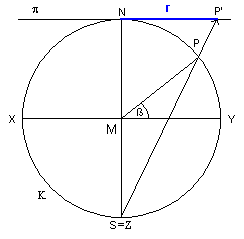
\includegraphics{img/stereo}
 \end{center}
 
 Das heißt, alle Punkte $x \in \Gamma$ werden auf den Punkt der Hyperebene
 abgebildet, an dem die Verbindungsgerade zwischen $x$ und $x_0$ die Ebene
 schneidet. Da für $x_0$ keine solche Gerade mit sich selbst  existiert,
 vereinbart man $\varphi(x_0) = \infty$.

 $\varphi$ ist offenbar bijektiv.
\end{defn*}

\subsection{Inversion (Spiegelung) an Hypersphären einer Sphäre}
Sei $\Gamma \subseteq \real^{n+1}$ eine $n$-Sphäre und $\Sigma \subseteq \Gamma$
eine $(n-1)$-Sphäre (\emph{Hypersphäre} in $\Gamma$). Dann ist $\Sigma = \Gamma
\cap H$ für eine Hyperebene $H$.

Falls $H$ durch den Mittelpunkt $a$ von $\Gamma$ geht, nennt man $\Sigma$ eine
\emph{Großhypersphäre}, anderenfalls eine
\emph{Kleinhypersphäre}.

Betrachte zum Beispiel die Einheitskugel in $\real^3$. Schnitte mit Ebenen
ergeben immer Kreise, dies sind die Hypersphären. Geht die Schnittebene durch 0,
ist es eine Großhypersphäre.

\begin{defn*}
 Die \emph{Inversion (Spiegelung) an der Hypersphäre $\Sigma$} ist für eine
 Kleinhypersphäre $\Sigma$ definiert durch $\Phi_\Sigma: \Gamma \to \Gamma$.
 
 Betrachte die Spitze $x_0$ des Tangentialkegels, der $\Gamma$ in $\Sigma$
 berührt. $\Phi_\Sigma$ vertauscht die beiden Schnittpunkte eines Strahls von
 $x_0$ durch einen Punkt aus $\Gamma \setminus \Sigma$ und bildet alle $x \in
 \Sigma$ auf sich ab.

 Betrachte zum Beispiel wieder die Einheitskugel im $\real^3$. An einen Kreis
 auf der Kugel kann man einen Tangentialkegel anlegen. alle Strahlen von der
 Spitze des Kegels durch die Kugel haben zwei Schnittpunkte, diese werden von
 $\Phi$ miteinander vertauscht. Die Strahlen auf den Kreis haben nur einen
 Schnittpunkt, da der Kegel die Kugel tangential berührt. Sie werden also auf
 sich selbst abgebildet.

 \begin{center}
  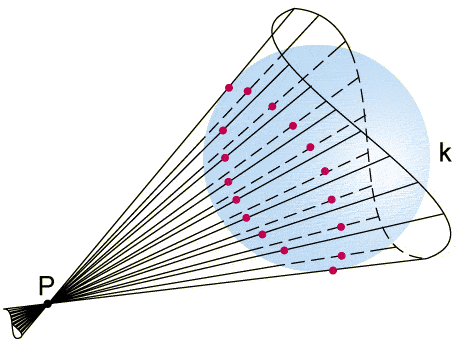
\includegraphics[width=.5\textwidth]{img/tangentialkegel}
 \end{center}
 
 Falls $\Sigma$ eine Großhypersphäre von $\Gamma$ ist, also $\Sigma = \Gamma \cap H$, $H$ Hyperebene durch den Mittelpunkt von $\Gamma$, dann ist $\Phi_\Sigma$ als die Einschränkung der Spiegelung an $H$ definiert.
\end{defn*}

Bezeichne $S(X) := \{ f : X \to X : f$ bijektive Abbildung $\}$.

\begin{defn*}
 Die \emph{verallgemeinerte Möbiusgruppe} $GM(\hat{\real}^n)$ ist definiert als die Untergruppe von $S(\hat{\real}^n)$, die von den Inversionen an Sphären und Spiegelungen an Hyperebenen erzeugt wird. Analog definiert man für die Sphäre $\sphere^n$ die Gruppe $GM(\sphere^n) = S(\sphere^n)$ als die Gruppe, die von Inversionen an Hyperebenen erzeugt wird. 
 \[ \sphere^n = \{ x \in \real^{n+1} : \| x \| = 1 \} \]
 Wir werden sehen, dass $GM(\sphere^n) \simeq GM( \hat{\real}^n )$.
\end{defn*}

\begin{defn*}
  Eine \emph{konforme} Abbildung $f: \real^m \to \real^m$ bewahrt Winkel, also
  \[ \angle(x,y) = \angle(f(x),f(y)). \]

  Eine differenzierbare Abbildung $f: \real^m \to \real^m$ heißt im Punkt $x_0$
  \emph{winkeltreu}, wenn die lineare Approximation $D_{x_0}f$ winkeltreu ist.
  $f$ heißt \emph{winkeltreu} oder \emph{konform}, falls $f$ für alle $x_0 \in
  \real^m$ in $x_0$ winkeltreu ist.

  Die lineare Abbildung $f: \real^m \to \real^m$ ist winkeltreu
  $\Leftrightarrow$ Es existiert $\lambda \ne 0$: $\lambda f$ ist
  orthogonal\footnote{Orthogonale Abbildungen erhalten das Skalarprodukt, sind
    also winkel- und längentreu.}.
\end{defn*}

\clearpage

\begin{thm}
 Sei $\Gamma$ die $n$-Sphäre $\{ x \in \real^{n+1} : \| x-a \| = r \} \subseteq \hat{\real}^{n+1}$. Sei $\Phi_\Gamma: \hat{\real}^{n+1} \to \hat{\real}^{n+1}$ die Inversion an $\Gamma$. Sie hat folgende Eigenschaften:
 \begin{enumerate}[1)]
  \item Sie bildet jede Hyperebene $H$ durch $a$ auf sich selbst ab und operiert auf $H$ als Inversion an $H \cap \Gamma$ ($H \cup \{ \infty \} =: H$)
  \item Sie vertauscht $n$-Sphären $\Sigma$ durch $a$ mit Hyperebenen $H$, die nicht durch $a$ gehen und die Einschränkung auf $\Sigma$ ist die stereographische Projektion von $a$ aus.
  \item Sie bildet die Menge der $n$-Sphären, die nicht durch $a$ gehen, in sich selbst ab.
  \item Sie bildet die Menge der $m$-Sphären und $m$-dimensionalen affinen Unterräume auf sich selbst ab ($0 \le m \le n$).
  \item $\Phi_\Gamma$ ist eine konforme Abbildung.
 \end{enumerate}
\end{thm}

\begin{proof}
  Wir betrachten o.B.d.A. $\Gamma = \Gamma_0$.

  Hyperebenen und Sphären werden durch die Gleichung
  \[ c \| x \|^2 + \angles{b,x} + d = 0 \]
  beschrieben. Die Lösungsmenge ist für
  \begin{itemize}
    \item $c = 0$ eine Hyperebene (falls $b \ne 0$),
    \item $c = 0$, $d \ne 0$ eine Hyperebene durch 0,
    \item $c \ne 0$, $d = 0$ eine Sphäre durch 0.
  \end{itemize}
  Wende die Abbildung $\Phi_{\Gamma_0}(x)$ mit $x \to \frac{x}{\|x\|^2}$ auf die Menge an. Es ergibt sich die Menge, die durch die Gleichung 
  \[ \frac{c}{\| x \|^2} + \frac{\angles{b,x}}{\| x \|^2} + d = 0, \qquad c + \angles{b,x} + d \| x \|^2 = 0 \]
  beschrieben wird. Also haben sich die Rollen von $c$ und $d$ vertauscht.

  Dies beweist die Aussagen 1) bis 3) bis auf die Aussagen über die
  Einschränkungen.

  Zu 1) Die Einschränkung der Spiegelung an $\Gamma$ auf $H \cup \{ \infty \}$
  ist eine Inversion an $H \cap \Gamma$, da es dieselbe Konstruktion ist.
  
  Zu 2) siehe Skizze (rechter Teil). Die Inversion wird am roten Kreis
  ausgeführt, Kreise durch den Mittelpunkt werden auf Hyperebenen abgebildet,
  die nicht den Mittelpunkt berühren.
  
  Die linke Seite illustriert 3), $n$-Sphären, die nicht durch $a$ gehen, werden
  auf andere $n$-Sphären abgebildet, die auch nicht $a$ berühren.
  
  \begin{center}
    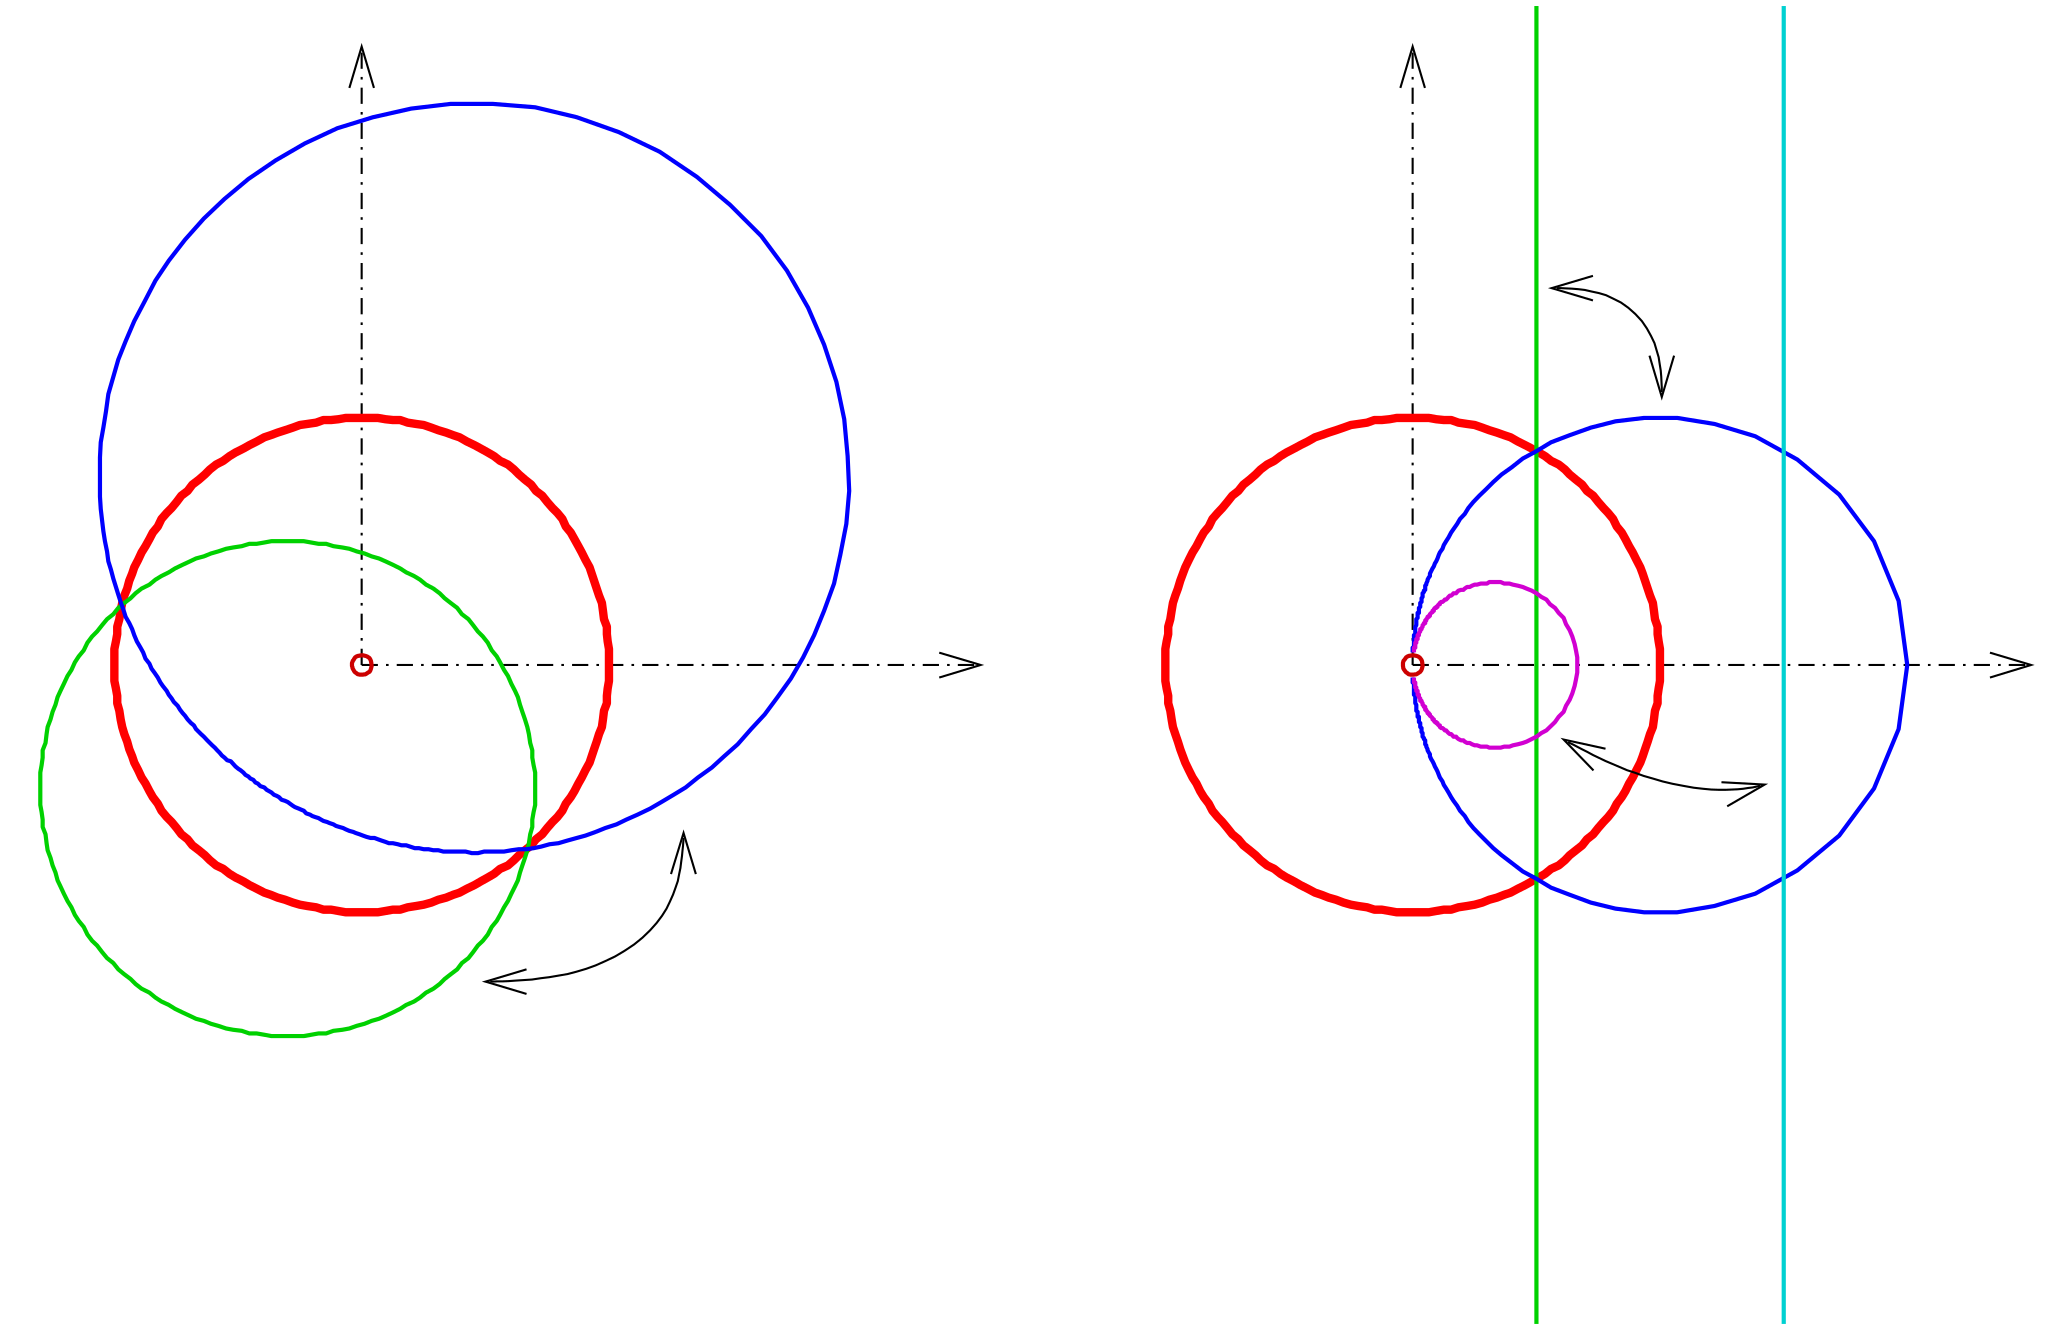
\includegraphics[width=.75\textwidth]{img/Inv-kreis-gerade}
  \end{center}

  Zu 4) Das folgt aus 1) bis 3) durch Bildung von Durchschnitten. $m$-Sphären
  bzw. $m$-dimensionale affine Unterräume (inklusive $\infty$) lassen sich als
  Schnitt von $n$-Sphären beziehungsweise Hyperebenen im $\real^{n+1}$
  darstellen und $\Phi_\Gamma$ ist eine bijektive Abbildung.

  Zu 5) Sei $x \in \real^n$, zunächst $x \notin \Gamma$ und seien zwei
  Tangentialrichtungen $v_1, v_2$ in $x$ gegeben. Betrachte die (eindeutig
  bestimmten) Kreise durch $x$ und $x' = \Phi_\Gamma(x)$, die jeweils in $x$ die
  gegebene Tangentialrichtung haben. (Sonderfall: Gerade, falls $v_i$ in
  Richtung von $\pm(x-x')$ zeigt.)

  $\Phi_\Gamma$ bildet jeden der beiden Kreise auf sich selbst ab, da der
  Bildkreis durch $\Phi_\Gamma(x)$, $x$ und den Schnittkreis durch $\Gamma$ geht
  und ein Kreis durch drei Punkte eindeutig bestimmt ist.

  Zwei Kreise, die sich schneiden, tun das an zwei Punkten und immer im selben
  Winkel. Damit folgt, dass $\Phi_\Gamma$ winkeltreu ist.
\end{proof}

\begin{defn*}
 Seien $x_1, \ldots, x_4 \in \hat{\real}^n$ paarweise verschieden. Dann
 definiere das \emph{Doppelverhältnis} 
 \[ \operatorname{DV}(x_1, x_2, x_3, x_4) := \frac{ \| x_1 - x_2 \| \cdot \| x_3
     - x_4 \| }{ \| x_1 - x_3 \| \cdot \| x_2 - x_4 \| }. \] 
 Achtung: Die Definition ist in der Literatur nicht ganz einheitlich, was die
 Reihenfolge der Punkte betrifft. 

 Falls ein Punkt $\infty$ ist, definiere zum Beispiel
 \[ \operatorname{DV}(x_1, x_2, x_3, \infty) := \frac{\|x_1 - x_2\|}{\|x_1 - x_3\|}. \]
\end{defn*}

Betrachte $x_1, x_2 \in \real^{n+1} \setminus \{ 0 \}$ und o.B.d.A. $f := \Phi_{\Gamma_0},$
\[ f(x) = \frac{x}{\|x\|^2}, \qquad f(0) = \infty, \qquad f(\infty) = 0. \]
Es gilt
\[ \begin{aligned}
    \| f(x_1) - f(x_2) \| 
    &= \left\| \frac{x_1}{\|x_1\|^2} - \frac{x_2}{\|x_2\|^2} \right\| \\
    &= \rez{ \| x_1 \| \cdot \| x_2 \|} 
       \left\| \frac{\| x_2 \|}{\| x_1 \|} x_1 - \frac{\| x_1 \|}{\| x_2 \|} x_2 \right\| \\
    &= \rez{ \| x_1 \| \cdot \| x_2 \|} \sqrt{\| x_2 \|^2 - 2 \angles{x_1,x_2} + \| x_1 \|^2} \\
    &= \frac{ \| x_1 - x_2 \| }{ \| x_1 \| \cdot \| x_2 \| }.
   \end{aligned} \]

Damit erhalten wir
\[ \DV( f(x_1), f(x_2), f(x_3) f(x_4) ) = \frac{ \| x_1 - x_2 \| \cdot \| x_3 -
    x_4 \| }{ \| x_1 - x_3 \| \cdot \| x_2 - x_4 \| } = \DV( x_1, x_2, x_3, x_4
  ). \]
Das Doppelverhältnis ist also invariant unter Inversion an der Einheitssphäre.
Für Inversionen an beliebigen Sphären ist das ``o.B.d.A.'' gerechtfertigt, da
Translationen und Streckungen das Doppelverhältnis offensichtlich bewahren. 

Falls ein $x_i$ gleich 0 oder $\infty$ ist, erfolgt die Rechnung mit der obigen
Definition analog. 

\addtocounter{thm}{-1}
\begin{thm}[Fortsetzung]
 \begin{enumerate}[1)]
  \setcounter{enumi}{5}
  \item Die Inversion an einer Sphäre bewahrt das Doppelverhältnis von vier
    verschiedenen Punkten. 
  \item Die Inversion an $\Gamma$ bildet jede $n$-Sphäre $\Sigma$, die $\Gamma$
    senkrecht schneidet auf sich selbst ab und operiert auf $\Sigma$ als
    Inversion an $\Gamma \cap \Sigma$.
  \item Die Inversion an einer Sphäre $\Gamma$ bzw. an der Hyperebene $\Gamma$
    ist dadurch charakterisiert, dass sie $\Gamma$ punktweise fest lässt und die
    beiden Schnittpunkte von sich schneidenden Kreisen, welche $\Gamma$
    senkrecht schneiden, miteinander vertauscht.
  \item $\Phi_{\Phi_\Gamma(\Sigma)} = \Phi_\Gamma \Phi_\Sigma \Phi_\Gamma$
    (beachte $\Phi_\Gamma^{-1} = \Phi_\Gamma$). 
  \item Die stereographische Projektion $\varphi: \Gamma \to \Pi \cup \{ \infty
    \}$ lässt sich zu einer Inversion $\Phi_\Sigma$ auf $\real^{n+1}$ fortsetzen
    (wobei $\Gamma \subseteq \hat{\real}^{n+1}$ Hypersphäre, $\Pi \subseteq
    \real^{n+1}$ Hyperebene). Folglich hat die stereographische Projektion
    ebenfalls die Eigenschaften 4) - 6). 
  \item Seien $\Gamma, \Gamma' \subseteq \hat{\real}^n$ zwei $k$-Sphären oder
    $k$-Ebenen ($k$-dimensionale affine Unterräume inklusive $\infty$). Dann ist
    in natürlicher Weise $GM(\Gamma) \subseteq GM(\hat{\real}^n)$. Ferner sind
    $GM(\Gamma)$ und $GM(\Gamma')$ in $GM(\hat{\real}^n)$ konjugierte
    Untergruppen, also insbesondere $GM(\Gamma) \simeq GM(\Gamma')$ und $GM(S^n)
    \simeq GM(\hat{\real}^n)$. 
  \item Alle Abbildungen in $GM(\hat{\real}^n)$ (verallgemeinerte
    Möbiustransformationen) erfüllen 4) - 6). 
 \end{enumerate}
\end{thm}

\begin{proof}
 \begin{enumerate}[1)]
  \setcounter{enumi}{5}
  \item Wurde bereits gezeigt.
  \item Das folgt direkt aus 3) und 5).
  \item Klar mit 3) und 5).
  \item Das folgt aus 8): Sei $x \in \hat{\real}^n$ beliebig.
  
  Betrachte zwei Kreise, die sich in $x$ schneiden und $\Phi_\Gamma(\Sigma)$ senkrecht schneiden. Sie schneiden sich also das zweite Mal in $\Phi_{\Phi_\Gamma(\Sigma)}$. 
  
  Die Bilder dieser Kreise unter $\Phi_\Gamma$ schneiden $\Phi_\Gamma(\Phi_\Gamma(\Sigma)) = \Sigma$ senkrecht und schneiden sich in $\Phi_\Sigma(x)$ und folglich das zweite Mal in $\Phi_\Sigma \Phi_\Gamma(x)$. Daraus folgt, dass für alle $x$ $\Phi_\Sigma \Phi_\Gamma(x)$ mit $\Phi_\Gamma \Phi_{\Phi_\Gamma(\Sigma)}(x)$ übereinstimmt und damit ist
  \[ \Phi_{\Phi_\Gamma(\Sigma)}= \Phi_\Gamma^{-1} \Phi_\Sigma \Phi_\Gamma = \Phi_\Gamma \Phi_\Sigma \Phi_\Gamma. \]
  \item Betrachte eine Sphäre $\Sigma$ mit Mittelpunkt $a \in \Gamma$. Die
    Inversion an dieser Sphäre operiert auf $\Gamma$ als stereographische
    Projektion.
  \item $GM(\hat{\real}^n)$ enthält alle Spiegelungen an Hyperebenen, also alle
    Bewegungen. Ferner ent\-hält sie alle Streckungen (betrachte einfach die
    Konjugation von zwei Inversionen an konzentrischen Sphären). Mit einer
    Inversion können wir einen $k$-dimensionalen affinen Unterraum auf eine
    $k$-dimensionale Sphäre abbilden und umgekehrt.
  
    Damit folgt 11) aus 9).
  \item Das ist klar, da die Eigenschaften in 4) bis 6) unter Komposition
    erhalten bleiben. \qedhere
 \end{enumerate}
\end{proof}

\textbf{Anwendungsbeispiel.} Gegeben sei eine Kreisschar durch zwei Punkte. Gibt
es eine weitere Kreisschar, die alle Kreise der ersten Schar senkrecht
schneidet? Wende die Inversion an einem Kreis an, der einen der beiden Punkte als
Mittelpunkt hat.

Inversionen an Sphären und Spiegelungen an Hyperebenen sind
orientierungsumkehrend. Eine Untergruppe vom $GM(\hat{\real}^n)$ sind daher auch
die orientierungserhaltenden Abbildungen in $GM(\hat{\real}^n)$.

Dies ist die Gruppe aller Kompositionen einer geraden Anzahl von Inversionen
(oder Spiegelungen an Hyperebenen). Diese Untergruppe $M(\hat{\real}^n)$ heißt
die Gruppe der Möbius\-trans\-formationen (meistens $M(\hat{\complex})$).

$M(\hat{\real}^n)$ enthält alle Translationen, Streckungen, Drehungen
(Inversionen an zwei konzentrischen Kreisen). In $\complex$:
\begin{itemize}
  \item $z \mapsto z + t$ ... Translation
  \item $z \mapsto a \cdot z$ ... Drehstreckung für $a \in \complex \setminus \{
    0 \}$
  \item $z \mapsto \rez{z}$ ... Komposition der Inversion am Einheitskreis in
    $\hat{\complex}$ mit der Spiegelung an der reellen Achse. ($\rez{z} = \frac{\obar{z}}{|z|^2}$)
\end{itemize}

Die Abbildungen dieser Art erzeugen die Möbiusgruppe $M(\hat{\complex})$ mit
\[ M(\hat{\complex}) = \left\{ f: \hat{\complex} \to \hat{\complex} : f(z) = \frac{ az +
    b}{c z + d} \text{ mit } ad - bc = 1 \right\}. \]
Weitere Diskussion in der Übung.

\subsection{Sphärische und elliptische Geometrie}
Wir betrachten die Geometrie auf $\sphere^n \subseteq \real^{n+1}$
(Einheitssphäre). Die Metrik auf $\sphere^n$ wird definiert durch
\[ d(x,y) = \arccos \angles{x,y} \qquad \in [0,\pi] \]
für $x,y \in \sphere^n$ (also $\| x \| = \| y \| = 1$).

Es gilt:
\begin{enumerate}
  \item $d$ ist eine Metrik auf $\sphere^n$.
  \item $d(x,y) + d(y,z) = d(x,y)$ $\Leftrightarrow$ $x,y,z$ liegen auf einem
    Großkreis (also sind $x,y,z$ linear abhängig) und $d(x,y) + d(y,z) \le
    \pi$ ($y$ liegt auf dem kürzeren Bogen, der $x$ und $z$ verbindet).
  \item Der kleinere der beiden Großkreisbögen, die $x$ und $y$ verbinden, hat
    Länge $d(x,y)$ und ist der kürzeste Abstand.
  \item Die Großkreise sind also die lokal kürzesten Verbindungen (in der
    Differentialgeometrie: geodätisch).
\end{enumerate}

\subsection{Geodätische Dreiecke auf der \texorpdfstring{$\sphere^2$}{S2}}

Seien $x,y,z$ drei Punkte auf $\sphere^2$, so dass $x,y,z,-x,-y,-z$ paarweise
verschieden sind.

Verbinde $x$ mit $y$, $y$ mit $z$ und $z$ mit $x$ durch die kürzesten
Verbindungen. Dadurch werden Zweiecke aufgespannt, die $x$ und $-x$, $y$ und
$-y$ sowie $z$ und $-z$ verbinden, ihre Öffnungswinkel seien $A$, $B$ und $C$.

Die Oberfläche der $\sphere^2$ ist $4 \pi$, der Flächeninhalt eines Zweiecks mit
Öffnungswinkel $A$ ist gleich $2A$.

Also folgt für die Fläche des Dreiecks $\Delta$:
\begin{align*}
    \Delta + \Delta_A &= 2A \tag{1} \\
    \Delta + \Delta_B &= 2B \tag{2} \\
    \Delta + \Delta_C &= 2C \tag{3} \\
    2(\Delta + \Delta_A + \Delta_B + \Delta_C) &= 4 \pi. \tag{4}
\end{align*}

Mit $(1) + (2) + (3) - \rez{2} (4)$ erhält man
\[ 2 \Delta = 2 (A+B+C) - 2 \pi, \]
also
\[ \Delta = A + B + C - \pi. \]

Wir haben damit gezeigt:

\newpage

\begin{thm}
  Der Flächeninhalt eines geodätischen Dreiecks auf der $\sphere^2$ ist
  \[ \Delta = A + B + C - \pi, \]
  wobei $A,B,C$ die drei Winkel des Dreiecks sind.
\end{thm}

Sei $x,y,z$ ein geodätisches Dreieck mit Seitenlänge $< \pi$. Die Winkel des
Dreiecks seien $A,B,C$, die Seiten $a,b,c$.

Ein \emph{Tangentialvektor} in $x$ ist gegeben durch
\[ u_1 = \frac{y-\angles{y,x}x}{\|y-\angles{y,x}x\|}, \]
denn $u_1 \perp x$, $\| u_1 \| = 1$, $\angles{u_1,y} = 0$. Analog folgt
\[ u_2 = \frac{z-\angles{z,x}x}{\|z-\angles{z,x}x\|}. \]

Nun können wir den Öffnungswinkel $A = \arccos \angles{u_1, u_2}$ bestimmen:
\[ \cos A = \angles{u_1,u_2} =
  \frac{\angles{y,z} - \angles{y,x} \angles{x,z}
    - \angles{z,x} \angles{x,y} + \angles{y,x} \angles{z,x}}
  {\sqrt{1 - 2 \angles{y,x}^2 + \angles{y,x}^2} \cdot
    \sqrt{1 - 2 \angles{z,x}^2 + \angles{z,x}^2} }. \]
Wegen $\sqrt{1 - \angles{y,x}^2} = \sqrt{1 - \cos^2 c} = \sin c$ und analog für
$\sin b$, $\cos c$ und $\cos b$ gilt also der sogenannte \emph{Kosinussatz}:
\[ \cos A = \frac{ \cos a - \cos b \cdot \cos c }{ \sin b \cdot \sin c }. \]

Es gilt
\[ \begin{aligned}
    \sin A &= \sqrt{1-\cos^2 A} \\
    &= \frac{\sqrt{\sin^2 b \sin^2 c - (\cos a - \cos b \cos c)^2}}{\sin b \cdot
      \sin c} \\
    &= \frac{\sqrt{(1-\cos^2 b)(1-\cos^2 c) - \cos^2 a + 2 \cos a \cos b \cos c
        - \cos^2 b \cos^2 c}}{\sin b \cdot \sin c} \\
    &= \frac{\sqrt{1 - \cos^2 a - \cos^2 b - \cos^2 c + 2 \cos a \cos b \cos
        c}}{\sin b \cdot \sin c}.
  \end{aligned} \]
Man kann die Berechnung analog für $B$ und $C$ durchführen und erhält
\[ \frac{\sin A}{\sin a} = \frac{\sin B}{\sin b} = \frac{\sin C}{\sin c}. \]

\subsection{Elliptische Geometrie}
Betrachte
\[ \begin{aligned}
    \proj(\real^{n+1}) &= \{ [x] : x \in \real^{n+1} \setminus \{0\}\} \\
    &= \{ [x] : x \in \sphere^1 \} = \sphere^n_\pm.
  \end{aligned} \]
Die natürliche Metrik auf $\real^{p^n}$ ($\proj(\real^{n+1})$ mit Längen und
Winkeln) ist
\[ d( [x], [y] ) = \arccos | \angles{x,y} | \le \frac{\pi}{2} \]
für $x, y \in \sphere^n$.

Die Geraden sind die Großkreise mit gegenüberliegenden Punkten identifiziert,
haben also Länge $\pi$.

In $\real^{p^2}$ gibt es ``nicht nullhomotope Dreiecke''.

\subsection{Modelle des hyperbolischen Raumes}
Der hyperbolische Raum wird mit $\real H^n$ bezeichnet.

\textbf{1. Modell.} (Klein'sches Modell, e-Modell)
\begin{itemize}
  \item Menge der \emph{Punkte}: Offene Einheitskugel
  \item \emph{Geraden} sind nichtleere Schnitte von Geraden in $\real^n$ mit $B^n$.
  \item Zwei Geraden (in diesem Modell) heißen \emph{parallel}, wenn sie sich
    auf dem Rand von $B^n$ schneiden.
\end{itemize}

\textbf{Inzidenzgeometrische Eigenschaften.}
\begin{itemize}
  \item Durch je zwei Punkte geht genau eine Gerade.
  \item Je zwei Geraden schneiden sich in höchstens einem Punkt.
  \item Zu jeder Geraden und jedem Punkt, der nicht auf der Geraden liegt, gibt
    es genau zwei Parallelen.
\end{itemize}


\textbf{Achtung!} Parallelität ist im $\real H^n$ \emph{keine
  Äquivalenzrelation}. Sinnvoller wäre es also, statt Geraden Strahlen zu
betrachten und parallele Strahlen.

\textbf{2. Modell} (Projektives Modell, p-Modell)
\begin{itemize}
  \item Fasse $B^n$ als Teilmenge von $\proj(\real^{n+1})$ auf.
  \[ x (\in \real^n) \quad \mapsto \quad \left[ \pmat{1 \\ x} \right] (\in
    \proj(\real^{n+1})). \]
  \item Menge der Punkte: $\real H^n := \left\{ \left[ \pmat{1 \\ x} \right]
      : x \in \real^n, \| x \| < 1 \right\}$.
  \item \emph{Geraden} sind nichtleere Schnitte von Geraden im
    $\proj(\real^{n+1})$ mit $\real H^n$.
  \item \emph{$k$-dimensionale Unterräume} sind nichtleere Schnitte von
    $k$-dimensionalen projektiven Unterräumen mit $\real H^n$.
\end{itemize}

Wir betrachten nun den $\real^{n+1}$ mit einer anderen Bilinearform, nämlich
\[ \angles{x,y}_- := x_1 y_1 - \sum_{j=2}^{n+1} x_j y_j, \]
wobei $x = (x_1, \ldots, x_{n+1})$ und $y = (y_1, \ldots, y_{n+1})$. Definiere
\[ J := \pmat{
    1 & 0 & \cdots & 0 \\
    0 & -1 \\
    \vdots & & \ddots \\
    0 & & & -1
  }. \]
Das ist die zu $\angles{\cdot,\cdot}_-$ gehörige Matrix.
\[ \angles{x,y}_- = x^T J y, \qquad \| x \|_- := \sqrt{|\angles{x,x}_-|}. \]

Nun können wir den $\real H^n$ so betrachten:
\[ \begin{aligned}
    \real H^n &= \{ [x] : x \in \real^{n+1}, \angles{x,x}_- > 0 \} \\
  &= \left\{ \left[ \pmat{ 1 \\ x_2 \\ \cdots \\ x_{n+1} } \right] : x_2^2 +
    \ldots + x_{n+1}^2 < 1  \right\} \\
  &= \{ [x] : x \in \real^{n+1}, \angles{x,x}_- = 1, x_1 > 0 \}.
\end{aligned} \]
Die Gleichung
\[ x_1^2 - x_2^2 - \ldots - x_{n+1}^2 = 1 \]
beschreibt ein zweischaliges Rotationshyperboloid.

\textbf{Zur Erinnerung.} Aus der Analysis ist bekannt
\begin{align*}
  \cos a &= \rez{2} (e^{ia} + e^{-ia}) & \cosh a &= \rez{2} (e^a + e^{-a}) \\
  \sin a &= \rez{2i} (e^{ia} - e^{-ia}) & \sinh a &= \rez{2} (e^a - e^{-a}),
\end{align*}
sowie
\[ \cosh^2 a - \sinh^2 a = 1. \]

Die Umkehrfunktionen sind
\begin{align*}
  \operatorname{arcosh} a &= \ln( a + \sqrt{a^2 - 1}), \\
  \operatorname{arsinh} a &= \ln( a + \sqrt{a^2 + 1}).
\end{align*}

\begin{defn*}
  Der hyperbolische Abstand von $[x]$, $[y] \in \real H^n$ ist
  \[ d([x],[y]) := \operatorname{arcosh} \frac{|\angles{x,y}_-|}{\|x\|_- \|y\|_-}.\]
  Wir müssen nachweisen, dass dadurch eine Metrik definiert ist. Dass $d(\cdot, \cdot)$ wohldefiniert, symmetrisch und $\ge 0$ ist, ist klar.

  Seien $x =\pmat{x_1 \\ \tilde{x}}$, $y =\pmat{y_1 \\ \tilde{y}}$ mit $x_1, y_1
  > 0$. O.B.d.A. sei $\angles{x,x}_- = \angles{y,y}_- = 1$. Dann gilt
  \[ x_1^2 - \| \tilde{x} \|^2 = y_1^2 - \| \tilde{y} \|^2 = 1. \]
  Damit folgt
  \[ \angles{x,y}_- = x_1 y_1 - \angles{\tilde{x},\tilde{y}} =\sqrt{1 + \|
      \tilde{x} \|^2} \cdot \sqrt{1 + \| \tilde{y} \|^2} -
    \angles{\tilde{x},\tilde{y}} \ge 0,\]
  denn
  \[ (1+\|\tilde{x}\|^2) (1+\|\tilde{y}\|^2) \ge ( 1 +
    \angles{\tilde{x},\tilde{y}})^2, \]
  wobei Gleichheit genau dann gilt, wenn $\tilde{x} = \tilde{y}$. Damit gilt
  $d(x,y) = 0$ genau dann, wenn $x = y$.
\end{defn*}

\subsection{Die Isometriegruppe von \texorpdfstring{$\real H^n$}{RH2}}
\begin{defn*}
  \begin{align*}
    O(1,n) 
    &= \{ A \in \real^{n+1,n+1} : A^T J A = J \} \\
    &= \{ A \in \real^{n+1,n+1} : \text{ Für alle $x,y \in \real^{n+1}$ gilt } 
      \angles{x,y}_- = \angles{Ax,Ay}_- \},
  \end{align*}
  denn
  \[x^T J y = \angles{x,y}_- = \angles{Ax,Ay}_- = x^T A^T J A y\]
  für alle $x,y \in \real^{n+1}$, also $A^T J  A = J$.

  Damit ist $A \in O(1,n)$, falls für die Spaltenvektoren $a_1, \ldots, a_{n+1}$
  gilt:
  \begin{align*}
    \angles{a_1, a_1}_- &= 1, \\
    \angles{a_i, a_i} &= -1 & \text{für alle } i = 2, \ldots, n+1, \\
    \angles{a_i, a_j} &= 0 & \text{für } i \ne j.
  \end{align*}
\end{defn*}

Für die Repräsentanten der Punkte in $\real H^n$ können wir voraussetzen $x_1
\ge 1.$

In $O(1,n)$ sind die linearen Abbildungen, die das zweischalige Hyperboloid $\{
x : \angles{x,y}_- = 1 \}$ auf sich abbilden.

Eine Untergruppe davon sind diejenigen, die jede der beiden Komponenten auf sich
abbilden, das heißt diejenigen Matrizen mit $a_{11} > 0$ (also sogar $a_{11} \ge
1$ wegen $\angles{a_1,a_1}_- = 1$).

\begin{defn*}
  \[ O_+(1,n) := \{ A \in O(1,n) : a_{11} > 0 \}. \]
  Die Abbildungen in $O_+(1,n)$ sind Isometrien des $\real H^n$, genauer ist für
  $A \in O_+(1,n)$ die Abbldung $[x] \mapsto [Ax]$ eine Isometrie.

  Die Abbildung $O_+(1,n) \to \operatorname{Iso}( \real H^n )$ ist injektiv.
\end{defn*}

\begin{defn*}
  Eine \emph{hyperbolische Spiegelung} (h-Spiegelung) ist eine Isometrie $f:
  \real H^n \to \real H^n$, die eine Hyperebene (punktweise) fest lässt, mit $f
  \ne \id$.
\end{defn*}

\begin{exmp*}
  Sei
  \[ A = \begin{pmatrix}
      \cosh s & - \sinh s & 0 & \cdots & 0 \\
      \sinh s & - \cosh s & 0 & \cdots & 0 \\
      0 & 0 & 1 \\
      \vdots & \vdots & & \ddots \\
      0 & 0 & & & 1
    \end{pmatrix}
  \]
  Wegen $\cosh^2 s - \sinh^2 s = 1$ ist $A \in O_+(1,n)$.

  Betrachte $\pmat{\cosh s & - \sinh s \\ \sinh s & - \cosh s}$. Wir ermitteln
  die Eigenwerte:
  \[ (\cosh s - \lambda)(- \cosh s - \lambda) + \sinh^2 s =
    - \cosh^2 s + \lambda^2 + \sinh^2 s = \lambda^2 -1 = 0. \]
  Also folgt $\lambda_{1,2} = \pm 1$.

  Bestimme nun einen Eigenvektor der Form $\pmat{ 1 \\ y }$ zu $\lambda_2 = -1$.
  Aus der ersten Zeile von
  \[ \pmat{\cosh s & - \sinh s \\ \sinh s & - \cosh s} \pmat{ 1 \\ y } = \pmat{
      1 \\ y } \]
  folgt $1 = - \cosh s + y \sinh s$ und damit
  \begin{align*}
    y &= \frac{1 + \cosh s}{\sinh s} = \frac{2 + e^s + e^{-s}}{e^s - e^{-s}} \\
      &= \frac{(e^{s/2} + e^{-s/2})^2}{(e^{s/2}+e^{-s/2})(e^{s/2}-e^{-s/2})}
        = \frac{e^{s/2}+e^{-s/2}}{e^{s/2}-e^{-s/2}} \\
    &= \coth \frac{s}{2}.
  \end{align*}
  Für $\lambda_1 = 1$ gilt $1 = \cosh s - y \sinh s$ und damit
  \[ y = \frac{-1 + \cosh s}{\sinh s} = \tanh \frac{s}{2}. \]

Also definiert $A$ im p-Modell eine h-Spiegelung und ist die Einschränkung einer
Zentralkollineation, deren Achse die Hyperebene
\[ \left\{ \left[ \pmat{ 1 \\ \tanh \frac{s}{2} \\ a } \right] : a \in
    \real^{n-1} \right\} \]
in $\proj( \real^{n+1})$ ist. Das Zentrum ist die Spitze des Tangentialkegels an
die Einheitskugel (in $\real H^n$) an den Schnitt der Hyperebene mit
$\obar{\real H}^n$,
\[ \left[  \pmat{1 \\ 0 \\ \vdots \\ 0} \right] \mapsto  \left[ \pmat{ \cosh s
      \\ \sinh s \\ \vdots \\ 0} \right] = \left[\pmat{ 1 \\ \tanh s \\ \vdots \\
      0}\right]. \]
\end{exmp*}

\begin{rmrk*}
Für $C \in O_+(1,n)$ gilt
\[ C \pmat{1 \\ 0 \\ \vdots \\ 0} = \pmat{1 \\ 0 \\ \vdots \\ 0} \qRq \exists B
  \in O(n) : C =
  \begin{pmatrix}
    1 & 0 & \cdots & 0 \\
    0 \\
    \vdots & & B \\
    0 
  \end{pmatrix}. \]
Wir betrachten die Matrizen in $O_+(1,n)$ als Isometrien des $\real H^n$,
nämlich $A([x]) := [Ax]$.
\end{rmrk*}

\begin{thm}
  \begin{enumerate}[a)]
  \item $O_+(1,n)$ operiert transitiv auf der Menge der Punktepaare von $\real
    H^n$ mit festem Abstand $a$.
  \item Jedes Element aus $O_+(1,n)$, lässt sich als Produkt von höchstens $n+1$
    h-Spiegelungen schreiben.
  \end{enumerate}
\end{thm}

\begin{proof}
  Zu a): Zunächst zeigen wir, dass jeder Punkt in $\real H^n$ durch eine
  h-Spiegelung auf $O := [ \pmat{1 & 0 & \cdots & 0}^T ]$ abgebildet werden
  kann.
  \[ A = \begin{pmatrix}
      \cosh s & - \sinh s & 0 & \cdots & 0 \\
      \sinh s & - \cosh s \\
      0 & 0 \\
      \vdots & \vdots & & E_{n-1} \\
      0 & 0
    \end{pmatrix}
    \qRq
  AO = \left[ \pmat{ \cosh s \\ \sinh s \\ \vdots \\ 0} \right] = \left[\pmat{ 1
      \\ \tanh s \\ \vdots \\ 0} \right]. \]
  Der Wertebereich von $\tanh s$ ist $(-1,1)$, also ist jeder Punkt der h-Geraden
  \[ \left[ \real \pmat{ 1 \\ 0 \\ 0 \\ \vdots \\ 0} + \real \pmat{ 1 \\ 1 \\ 0
        \\ \vdots \\ 0} \right] \cap \real H^n \]
  das Bild von $O$ unter einer h-Spiegelung der obigen Form.

  Sei $\left[ \pmat{1 \\ x} \right] \in \real H^n$ beliebig und $s =
  \operatorname{artanh} (\|x\|)$. Die h-Spiegelung an der Hyperebene orthogonal
  (im e-Modell) zu $x$ und durch $\frac{x}{\|x\|} \tanh \frac{s}{2}$ vertauscht
  $O$ und $\left[ \pmat{1 \\ x} \right]$.

  Seien nun $[x_1], [x_2], [y_1], [y_2] \in \real H^n$ mit $d([x_1],[x_2]) =
  d([y_1],[y_2])$. Dann gibt es $\varphi_1, \varphi_2 \in O_+(1,n)$ mit
  \[ \varphi_1(x_1) = \pmat{1 \\ 0 \\ \cdots \\ 0}, \qquad \varphi_2(y_1) =
    \pmat{1 \\ 0 \\ \cdots \\ 0}. \]
  Wegen
  \[ d(O, [\varphi_1(x_2)]) = d([\varphi_1(x_1)], [\varphi_1(x_2)]) =
    d([y_1],[y_2]) = d(O,[\varphi_2(y_2)]) \]
  gibt es $\varphi_3= \pmat{1 & 0 \\ 0 & B}$ mit $B \in O(n)$ mit $[\varphi_3
  \varphi_1(x_2)] = [\varphi_2(x_2)]$. Also bildet $\varphi_3^{-1} \circ
  \varphi_3 \circ \varphi_1$ $x_1$ auf $y_1$ und $x_2$ auf $y_2$ ab.

  Zu b): Sei $A \in O_+(1,n)$ beliebig und $x = A \cdot (1,0,\ldots,0)^T$. Dann
  gibt es eine h-Spiegelung $S_0$ mit $S_0 x = (1,0,\ldots,0)^T$. Damit gilt
  \[ S_0 A \cdot \pmat{1 \\ 0 \\ \vdots \\ 0} = \pmat{1 \\ 0 \\ \vdots \\ 0} \]
  und folglich ist $S_0 A$ von der Form $\pmat{1 & 0 \\ 0 & B}$ mit $B \in
  O(n)$. $B$ ist ein Produkt von höchstens $n$ Spiegelungen an Hyperebenen des
  $\real^n$.

  Eine Spiegelung im e-Modell an einer Hyperebene durch $O$ des $\real^n$ ist
  auch eine h-Spiegelung ($C \in O(n) \mapsto \pmat{1 & 0 \\ 0 & C}$). Also ist
  $A$ Produkt von höchstens $n+1$ h-Spiegelungen.
\end{proof}

\subsection{Das konforme Modell des hyperbolischen Raumes}
Stereographische Projektion
\[ \varphi: \sphere^n \to \hat{\real}^n, \qquad \varphi(x,t) = \frac{x}{1-t}, \]
wobei $t^2 + \|x\|^2 = 1$, $t \ne 1$. $\varphi(0,1) = \infty$.

\textbf{Übergang vom e-Modell zum k-Modell.} Dieser erfolgt durch eine geometrische
Konstruktion. Bilde zunächst $B^n$ auf die untere Halbsphäre der $\sphere^n
\subseteq \real^{n+1}$ durch orthogonale Projektion ab.

Bilde die untere Halbsphäre anschließend durch stereographische Projektion vom
Nordpol aus auf die offene Kugel $B^n$ ab.

Eine h-Gerade im e-Modell (Schnitt von Gerade mit $B^n$) wird durch die
orthogonale Projektion auf einen Kreisbogen abgebildet (auf der unteren
Halbsphäre), der den Rand von $B^n$ senkrecht schneidet. Durch die
stereographische Projektion (winkeltreu!) wird dieser Kreis auf einen Kreis oder
eine Gerade in $B^n$ abgebildet, der den Rand senkrecht schneidet.

Der Rand von $B^n$ bleibt unter beiden Abbildungen punktweise fest. Damit
erhalten wir das \emph{konforme Modell}.

\textbf{k-Modell.}
\begin{itemize}
  \item Menge der \emph{Punkte}: $B^n = \{ x \in \real^n : \| x \| \le 1 \}$
  \item \emph{Geraden} sind Schnitte von Kreisen, die $\partial B^n$ senkrecht
    schneiden mit $B^n$ bzw. Schnitte von Geraden durch 0 mit $B^n$.
  \item \emph{$m$-dimensionale Unterräume} sind Schnitte von $m$-Sphären, die
    $\partial B^n$ senkrecht schneiden, mit $B^n$.
\end{itemize}

\textbf{Direkter Übergang zwischen den Modellen.} Sei $x \in B^n$. Projektion
senkrecht nach unten auf $\sphere^n \subseteq \real^{n+1}$ ergibt
\[ \pmat{ x \\ - \sqrt{1-\|x\|^2}} \mapsto \frac{x}{1 + \sqrt{1-\|x\|^2}}, \]
wobei $\mapsto$ die stereographische Projektion ist.

Die Abbildung $F: B^n \to B^n$ ist definiert durch
\[ F(x) := \frac{x}{1+\sqrt{1-\|x\|^2}}. \]
Sie bildet $x$ im e-Modell auf den entsprechenden Punkt im k-Modell ab.

\begin{center}
\begin{tabular}{c|c|c}
  e-Modell & p-Modell & k-Modell \\
  \hline
  $x$ & $\left[ \pmat{1\\x} \right]$ & $\cfrac{x}{1+\sqrt{1-\|x\|^2}}$ \\[5pt]
  $\cfrac{x}{a}$ & $\left[ \pmat{a\\x} \right]$ & $\cfrac{x}{a+\sqrt{a^2-\|x\|^2}}$
\end{tabular}
\end{center}
mit $\|x\|^2 < a^2$.

Sei $H$ eine Hyperebene, die $B^n$ schneidet, bezeichne $\Psi_H$ die
$h$-Spiegelung an $H$ (im $e$-Modell), also ist $\Psi_H$ die Einschränkung der Zentralkollineation, welche $B^n$ auf sich abbildet mit Achse $H$ und deren Zentrum die Spitze des Tangentialkegels an $B^n$ in $\partial B^n \cap H$ ist.

\begin{thm}[Hyperbolische Spiegelungen im k-Modell]
 Sei $\Phi_{F(H)}$ die Inversion (Spiegelung) an der Sphäre $F(H)$. Dann gilt auf $B^n$:
 \[ F \circ \Psi_H = \Phi_{F(H)} \circ F, \]
 das heißt die h-Spiegelung an der h-Hyperebene $H \cap B^n$ im e-Modell entspricht genau der Inversion (Spiegelung) an der Sphäre $F(H)$ im k-Modell.
\end{thm}

\begin{proof}
 Auf dem Rand $\partial B^n$ stimmen $\Psi_H$ und $\Phi_{F(H)}$ überein.
 
 1. Fall: Für $x \in H$ ist $F(x) \in F(H)$, also $F \circ \Psi_H(x) = F(x) = O_{F(H)} F(x)$.
 
 2. Fall: Sei $x \in B^n \setminus H$. Sei $E$ die Ebene durch $0$, $x$ und $z$ (Zentrum von $\Psi_H$). $E$ schneidet $\partial B^n = \sphere^{n-1}$ in einem Großkreis. Wir können die Konstruktion in $E$ durchführen (Die Einschränkung von $E$ auf $\partial B^n$ wird unter den betrachteten Abbildungen auf sich abgebildet). 
 
 Die Konstruktion der Bildpunkte zeigt, dass $F \circ \Psi_H(x) = \Phi_{F(H)} F(x)$ gilt. Wir verwenden dabei, dass die Abbildungen $\Phi_{F(H)}$ und $\Psi_H$ auf $\partial B^n$ übereinstimmen und wegen der Winkeltreue von $\Phi_{F(H)}$ Kreise, die $\partial B^n$ senkrecht schneiden, wieder auf Kreise überführt werden, die $\partial B^n$ senkrecht schneiden.
\end{proof}

\begin{rmrk*}
 \begin{enumerate}[1)]
  \item Die Abbildungen $\Psi_H$ und $\Phi_{F(H)}$ auf $\sphere^{n-1} = \partial B^n$ sind die Inversion der $\sphere^{n-1}$ an $H \cap \sphere^{n-1}$.
  \item Jede Spiegelung der $\sphere^{n-1}$ an einer $(n-2)$-Sphäre $\Sigma \subseteq \sphere^{n-1}$ lässt sich einerseits \emph{ein\-deu\-tig} zu einer Spiegelung an der $(n-1)$-Sphäre, die die $\sphere^{n-1}$ in $\Sigma$ schneidet, fortsetzen, andererseits zu einer Zentralkollineation $\Psi_H$ mit $\Sigma = H \cap \sphere^n$.
 \end{enumerate}
\end{rmrk*}

\begin{thm}
 Die h-Winkel stimmen mit den Winkeln im k-Modell überein.
\end{thm}

\begin{proof}
 Zwei h-Strahlen $g_1$, $g_2$ von einem Punkt $x \in B^n$ lassen sich durch eine h-Spiegelung auf Strahlen abbilden, die von 0 (im e-Modell bzw. im k-Modell) ausgehen. Der Winkel $\alpha$ zwischen diesen Strahlen stimmt im e-Modell und im k-Modell überein und $\alpha$ ist auch der h-Winkel.
 
 Wir wissen, dass eine h-Spiegelung nach Satz 4.3 einer Inversion an einer Sphäre im k-Modell entspricht. Diese Inversionen sind winkeltreu, also stimmen auch die Winkel zwischen den h-Strahlen im k-Modell mit den Winkeln zwischen $g_1$ und $g_2$ überein.
\end{proof}

\begin{thm}
 Es gilt 
 \[ GM(\hat{\real}^n) \simeq GM( \sphere^n ) \simeq O_+ (1, n+1). \]
 Ferner gilt: Jede Möbiustransformation $f \in GM(\sphere^n)$ bzw. $f \in GM(\hat{\real}^n)$ lässt sich als Produkt von höchstens $n+2$ Spiegelungen an $(n-1)$-Sphären schreiben.
\end{thm}

\begin{proof}
 Wir haben schon gezeigt, dass $GM(\hat{\real}^n) \simeq GM( \sphere^n )$. Sei $f \in GM(\sphere^n)$, das heißt $f$ lässt sich als Produkt (Komposition) von Spiegelungen an $(n-1)$-Sphären darstellen.
 
 Diese lassen sich jeweils \emph{eindeutig} zu Zentralkollineationen fortsetzen, welche $B^{n+1}$ auf sich selbst abbilden (also h-Spiegelungen im e-Modell). Diese lassen sich jedoch durch eine Matrix $A \in O_+(1,n+1)$ darstellen. Damit ist $f$ die Einschränkung einer Kollineation $\obar{f}: \proj(\real^{n+2}) \to \proj(\real^{n+2})$ auf $O_+(1,n+1)$. 
 
 Diese Kollineation $\obar{f}$ ist durch $f$ eindeutig bestimmt: Sei $x \in \proj(\real^{n+2})$. Dann gibt es $a_1, a_2, b_1, b_2 \in \sphere^n (\subseteq \proj( \real^{n+2} ) )$ mit $x = a_1 a_2 \cap b_1 b_2$, also $f(\obar{x}) = f(a_1) f(a_2) \cap f(b_1) f(b_2)$.
 
 Damit erhalten wir eine Abbildung $\tilde{f}: GM(\sphere^n) \to O_+(1,n+1)$. Sie ist offenbar mit Komposition verträglich, also ein Gruppenhomomorphismus. 
 
 Ferner ist $\tilde{f}$ injektiv, da
 \[ f = \tilde{f}(f) | : \sphere^{n-1} \to \sphere^{n-1}. \]
 Das heißt, $f$ ist die Einschränkung von $\tilde{f}$ auf $\sphere^{n-1}$ (?)
 
 Andererseits ist $\tilde{f}$ auch surjektiv, da sich jede Abbildung in $O_+(1, n+1)$ nach Satz ... als Produkt von höchstens $n+2$ h-Spiegelungen darstellen lässt.
 
 Die von einer h-Spiegelung in $\real H^{n+1}$ induzierte Abbildung auf $\sphere^n$ ist eine Spiegelung an einer $(n-1)$-Sphäre. Also lässt sich $f \in GM( \sphere^n$ als Produkt von höchstens $n+2$ Spiegelungen an $(n-1)$-Sphären darstellen.
\end{proof}

\subsection{Der Flächeninhalt von Dreiecken in \texorpdfstring{$\real H^2$}{IRH2}}
\begin{defn*}
 Zwei Teilmengen $M_1$, $M_2$ in $\real H^n$ heißen \emph{kongruent}, wenn es eine Isometrie (in $O_+(1,n)$) $f: \real H^n \to \real H^n$ gibt mit $f(M_1) = M_2$.
 
 Ein Dreieck in $\real H^2$ heißt \emph{$k$-fach asymptotisch} ($k \in \{ 1, 2, 3 \}$), falls $k$ Ecken im ``Unendlichen'' liegen, also auf $\partial B^2$ im e-Modell bzw. k-Modell.
\end{defn*}

\begin{thm}
  \begin{enumerate}[a)]
  \item Für je drei (verschiedene) Punkte $x_1, x_2, x_3 \in \sphere^1$ und
    $x_1', x_2', x_3' \in \sphere^1$ gibt es $f \in GM(\sphere^1)$ mit $f(x_i) =
    i'$ für $i = 1,2,3$.
    Folglich sind je zwei dreifach asymptotische Dreiecke in $\real H^2$
    zueinander kongruent.
    \item Je zwei zweifach asymptotische Dreiecke in $\real H^2$ mit demselben
      Winkel $A$ sind zueinander kongruent.
    \item Der Flächeninhalt eines dreifach asymptotischen Dreiecks in $\real
      H^3$ ist $\pi$.
    \item Der Flächeninhalt eines zweifach asymptotischen Dreiecks mit Winkel $A
      \ne 0$ ist $\pi - A$.
    \item Der Flächeninhalt $\Delta$ eines beliebigen Dreiecks in $\real H^2$
      mit Winkeln $A,B,C$ ist
      \[ \Delta = \pi - (A+B+C). \]
  \end{enumerate}
\end{thm}

\begin{proof}
  %% Noch machen
\end{proof}

\clearpage
\setcounter{secnumdepth}{1}
\section{Quadriken}
\setcounter{secnumdepth}{0}
\begin{defn*}
  Eine \emph{Hyperfläche zweiter Ordnung} bzw. \emph{Quadrik} in $\real^n$ ist
  eine Menge der Form
  \[ Q = \{ x \in \real^n : x^T A x + 2 \angles{b,x} + c = 0\}, \]
  wobei $A \in \real^{n,n}$ sei mit $A^T = A$, $b \in \real^n$, $c \in \real$.

  Andere Schreibweise:
  \[ \pmat{x^T & 1} \cdot \pmat{A & b \\ b^T c} \cdot \pmat{x\\1} = 0. \]
\end{defn*}

Eine Quadrik ist also die Nullstellenmenge eine Polynoms zweiten Grades in $n$
Variablen.

\begin{exmp*}
  Die Gleichung
  \[ 9x^2 - 4 xy + 6 y^2 + 2x + 4y - 1 = 0 \]
  hat die äquivalente Darstellung
  \[ \pmat{x & y} \cdot \pmat{9 & -2 \\ -2 & 6} \cdot \pmat{x\\y} + 2
    \angles{\pmat{1\\2},\pmat{x\\y}} - 1  = 0. \]
\end{exmp*}

Zwei Mengen $M_1, M_2$ heißen \emph{affin äquivalent}, wenn es eine bijektive
affine Abbildung $\psi: \real^n \to \real^n$ gibt mit $\psi(M_1) = M_2$.

\textbf{Ziel:} Klassifikation der Quadriken bis auf Kongruenz, Resultat ist eine
``Normalform'' (bzgl. Isometrie).

\textbf{1. Schritt.} (Hauptachsentransformation) Wir wissen, dass wegen $A=A^T$
eine orthogonale Matrix $S \in O(n)$ existiert, so dass $S^T A S = S^{-1} A S =:
D$ eine Diagonalmatrix ist.

Wenn $(b_1, \ldots, b_n)$ eine Orthonormalbasis aus Eigenvektoren ist und $(d_1,
\ldots, d_n)$ die zugehörigen Eigenwerte, dann ist
\[ S = \pmat{b_1 & \cdots & b_n}, \qquad D = \pmat{d_1 & & 0 \\ & \ddots \\ 0 &
    & d_n}. \]

Seien o.B.d.A.. $d_1, \ldots, d_k \ne 0$, $d_{k+1} = \cdots = d_n = 0$, also $k
= \rang A$.

Die Transformation $\tilde{x} = S^T x = S^{-1} x$, also $x = S \tilde{x}$ ergibt
\[ 0 = x^T A x + 2 \angles{b,x} + c = \tilde{x}^T \underbrace{(S^T A S)}_{=D}
  \tilde{x} + 2 \underbrace{\angles{b, S \tilde{x}}}_{=\angles{S^T b, \tilde{x}}=\angles{\tilde{b},\tilde{x}}} + c. \]

\textbf{2. Schritt.} Ziel: In den Variablen $\tilde{x}_1, \ldots, \tilde{x}_k$
die linearen Terme durch eine Translation eliminieren.

Wir führen eine quadratische Ergänzung durch:
\[ d_i \tilde{x}_i^2 + 2 \tilde{b}_i \tilde{x}_i = d_i \left( \tilde{x}_i +
    \frac{\tilde{b}_i}{d_i} \right)^2 - \frac{\tilde{b}_i^2}{d_i}. \]
Nach dem zweiten Schritt haben wir eine Gleichung der Form
\[ \sum_{i=1}^k d_i x_i^2 + \sum_{i=k+1}^1 \tilde{b}_i x_i + \hat{c} = 0, \]
wobei $\hat{c} = c - \sum_1^k \frac{\tilde{b}_i^2}{d_i}$.

\textbf{3. Schritt.} Die vorhandenen linearen Terme zusammenfassen.

Für $\hat{c} \ne 0$ kann man im letzten Schritt die Gleichung so normieren, dass
o.B.d.A. der konstante Term -1 ist.

\textbf{1. Fall.}
\[ \frac{x_1^2}{a_1^2} + \cdots + \frac{x_h^2}{a_h^2} -
  \frac{x_{h+1}^2}{a_{h+1}^2} - \cdots - \frac{x_k^2}{a_k^2} = 1 \]
mit $0 \le h \le k \le n$. Falls $h = 0$ erhalten wir die leere Menge.

\textbf{2. Fall.}
\[ \frac{x_1^2}{a_1^2} + \cdots + \frac{x_h^2}{a_h^2} -
  \frac{x_{h+1}^2}{a_{h+1}^2} - \cdots - \frac{x_k^2}{a_k^2} = 0 \]
mit $0 \le h \le k \le n$ und $k-h \le h$ (ggf. muss man die Gleichung mit -1
multiplizieren).

\textbf{3. Fall.}
\[ x_{k+1} = \frac{x_1^2}{a_1^2} + \cdots + \frac{x_h^2}{a_h^2} -
  \frac{x_{h+1}^2}{a_{h+1}^2} - \cdots - \frac{x_k^2}{a_k^2} \]
mit $0 \le h \le k \le n$ und $k-h \le h$ (ggf. vertausche $x_{k+1}$ mit $-x_k$).

3. Fall: (Vorbereitung zu 5) $\hat{b} \ne 0$.
\[ \hat{x}^T D \hat{x} + \underbrace{\angles{\hat{b},\hat{x}}  + \tilde{c}}_{\| \hat{b} \| \cdot \hat{x}_{k+1}} = 0, \]
also
\[ \hat{x}_{k+1} = \angles{ \frac{\hat{b}}{\| \hat{b} \|}, \hat{x}} +
  \frac{\tilde{c}}{\hat{b}}. \]

\clearpage

\begin{thm}
  \begin{enumerate}[a)]
    \item Jede Quadrik in $\real^n$ ist kongruent zu genau einer der folgenden
      Mengen $\{x \in \real^n : $ Gleichung gilt $\}$:
      \begin{enumerate}[1)]
        \item $\emptyset$
        \item
          \[ \frac{x_1^2}{a_1^2} + \cdots + \frac{x_h^2}{a_h^2} -
            \frac{x_{h+1}^2}{a_{h+1}^2} - \cdots - \frac{x_k^2}{a_k^2} = 1 \]
          mit $1 \le h \le k \le n$, $a_1 \ge \ldots \ge a_h > 0$, $a_{h+1} \ge
          \ldots \ge a_k \ge 0$.
        \item
          \[ x_1^2 + \cdots + \frac{x_h^2}{a_h^2} -
            \frac{x_{h+1}^2}{a_{h+1}^2} - \cdots - \frac{x_k^2}{a_k^2} = 0 \]
          mit $1 \le h \le k \le n$, $k-h \le h$, $1 \ge \ldots \ge a_h > 0$, $a_{h+1} \ge \ldots \ge a_k \ge 0$.

          Achtung: Falls $k-h=h$, gibt es zwei solche Darstellungen kongruenter
          Mengen (multipliziere die Gleichung mit $-a_{h+1}^2$).
        \item
          \[ x_1^2 + \ldots + x_k^2 = 0 \]
          $(n-k)$-dimensionaler linearer Unterraum ($x_1 = x_2 =  \ldots = x_k =
          0$). 
        \item
          \[  \frac{x_1^2}{a_1^2} + \ldots + \frac{x_h^2}{a_h^2} -
            \frac{x_{h+1}^2}{a_{h+1}^2} - \ldots - \frac{x_k^2}{a_k^2} =
            x_{k+1}. \] 
          mit $1 \le h \le k \le n-1$, $k-h \le h$, $a_1 \ge a_2 \ge \ldots \ge
          a_h > 0$, $a_{h+1} \ge a_{h+2} \ge \ldots \ge a_k > 0$.

          Falls $k-h = h$, gibt es wieder  zwei Möglichkeiten (ersetze $x_{k+1}$
          durch $-x_{k+1}$).
    \end{enumerate}
    \item Jede Quadrik in $\real^n$ ist affin äquivalent zu genau einer der
      obigen Mengen, wobei alle vorkommenden $a_i = 1$ gesetzt werden.
  \end{enumerate}
\end{thm}

\textbf{Zum Beweis:}  Die Existenz wird über die Konstruktion der Normalform gezeigt.

Der Beweis der Eindeutigkeit wird weggelassen, ist aber anschaulich klar und nicht schwer zu
zeigen.

Zu b) vergleiche den Beweis zum Trägheitssatz von Sylvester.

\bigskip

\textbf{Beispiele.}
Wir betrachten nun die Möglichkeiten speziell für $n=2$:
\begin{itemize}
  \item $\frac{x^2}{a^2}+{y^2}{b^2} = 1$, Ellipse mit (Länge der) Halbachsen $a$ und $b$.
  \item $\frac{x^2}{a^2} - {y^2}{b^2} = 1$, Hyperbel mit Halbachse $a$ und Steigung der Asymptoten $\pm b/a$.
  \item $y = \frac{x^2}{2p}$, Parabel
  \item $-x^2 - y^2 = 1$, $\emptyset$.
  \item $x^2 + y^2 = 0$, Punkt.
  \item $\frac{x^2}{a^2} - \frac{y^2}{b^2} = 0$, äquivalent zu $x^2 -
      \frac{a^2}{b^2} y^2 = 0$, Paar sich schneidender Geraden.
  \item $\frac{x^2}{a^2} = -1$ $\Leftrightarrow$ $x = \pm a$ Paar paralleler
    Geraden.
  \item $x^2 = 0$ Gerade ($x=0$, $y$ beliebig).
\end{itemize}

\subsection{Ellipse und Hyperbel}
Betrachte die Lösungsmenge der Gleichung
\[ \frac{x^2}{a^2} + \eps \frac{y^2}{b^2} = 1, \]
wobei $\eps \in \{ -1, 1 \}$.

Für $\eps = 1$ handelt es sich um eine Ellipse mit Halbachsen $a,b$, sei $a \ge
b$. Für $\eps = -1$ ist es eine Hyperbel.

Die ``Brennpunkte'' sind $F_1 = (c,0)$, $F_2 = (-c, 0)$. Der Abstand der
Brennpunkte vom Mittelpunkt ist $c$, wobei
\[ c = \sqrt{a^2 - \eps b^2}. \]

Wir definieren zur Abkürzung
\[ e := \frac{c}{a} = \sqrt{1 - \eps \frac{b^2}{a^2}}. \]
Man nennt $e$ die (numerische) \emph{Exzentrizität} der Ellipse.

Die Abstände der Brennpunkte zu einem Punkt auf der Ellipse bzw. Hyperbel
$P = (x,y)$ werden mit $r_{1,2}$ bezeichnet. Mit der Definition von $e$ folgt
\[ r_1 = PF_1 = \sqrt{(x-c)^2 + y^2} = \sqrt{x^2 - 2cx + a^2 - \eps b^2 +
    y^2} \]
Setze ein $y^2 = \eps( b^2 - x^2 \cdot \frac{b^2}{a^2})$, da $(x,y)$ auf der
Kurve liegt, also
\[ r_1 = \sqrt{e^2 x^2 - 2 eax + a^2} =
  \begin{cases}
    a - ex, &\text{für } \eps = 1, \\
    ex - a, &\text{für } \eps = -1, (x,y) \text{ auf dem rechten Ast }(x \ge a).
  \end{cases} \]
Es folgt
\[ r_2 = PF_2 = a + ex\]
genau entsprechend (ersetze $e$ durch $-e$). Bei der Hyperbel ist wieder $(x,y)$
auf dem rechten Ast.

Also gilt
\[ r_2 + \eps r_1 = 2a \]
konstant, somit ist $r_1 + r_2 = 2a$ für $\eps = 1$ (Ellipse)
``Gärtnerkonstruktion''\footnote{Nehme einen Strick der Länge $2a$ und befestige
  ihn in $F_1$, $F_2$. Dann lässt sich eine Ellipse mit den gewünschten
  Eigenschaften abstecken.}.

Für $\eps = -1$ (Hyperbel, rechter Ast bei $x \ge a$) gilt $|r_2 - r_1| = 2a$
für beide Äste.

\begin{bem}
  Aus $e = \rez{2} \| F_2 - F_1 \| = \sqrt{a^2 - \eps b^2}$ folgt
  \[ b = \sqrt{ \eps \left( a^2 - \left( \frac{\| F_2 - F_1 \|}{2} \right)^2 \right) }
      = \sqrt{ \left| a^2 - \left( \frac{\| F_2 - F_1 \|}{2} \right)^2 \right| } \]
\end{bem}

\begin{prp}
  \begin{enumerate}[a)]
    \item $\{ x \in \real^2 : \| x - F_1 \| + \| x - F_2 = 2a \}$, wobei $2a >
      \| F_2 - F_1 \|$ sei, ist eine Ellipse mit den Brennpunkten $F_1$ und
      $F_2$. Die größere Halbachse hat die Länge $a$ und die kleinere Halbachse
      $b$ mit
      \[ b = \sqrt{a^2 - \left( \frac{\|F_2 - F_1 \|}{2} \right)^2 }. \]
    \item $\{ x \in \real^2 : \| x - F_1 \| - \| x - F_2 = 2a \}$, wobei $2a <
      \| F_2 - F_1 \|$ sei, ist eine Hyperbel mit den Brennpunkten $F_1$ und
      $F_2$, die kongruent ist zu
      \[ \left\{ \pmat{u \\ v} \in \real^2 : \frac{u^2}{a^2} - \frac{v^2}{b^2} =
          1 \right\} \]
      mit
      \[ b = \sqrt{\left( \frac{\|F_2 - F_1 \|}{2} \right)^2 - a^2}. \]
  \end{enumerate}
\end{prp}

\begin{proof}
  Das folgt aus den oben gezeigten Zusammenhängen.
\end{proof}

\begin{defn*}
  Eine Menge $M \subseteq \real^n$ heißt \emph{konvex}, wenn für je zwei Punkte
  $x,y \in M$ die Verbindungsstrecke $\{ \lambda x + (1-\lambda) y : \lambda \in
  [0,1] \} \subseteq M$ ist.
\end{defn*}

\begin{kor}
  \begin{enumerate}[a)]
    \item Falls $M$ konvex ist und $\varphi: \real^n \to \real^m$ eine affine
      Abbildung, dann ist auch $\varphi(M)$ konvex.
    \item Die Kugel $\{ x : \| x \| \le r \}$ ist konvex und damit ist auch das
      Vollellipsoid
      \[ \frac{x_1^2}{a_1^2} + \ldots + \frac{x_n^2}{a_n^2} \le 1 \]
      konvex.
    \item Falls $M \subseteq \real^2$ konvex und abgeschlossen ist und $T$ eine
      Tangente an $\partial M$ ist, dann liegt $M$ ganz in einem der beiden von
      $T$ begrenzten Halbräume.
    \end{enumerate}
\end{kor}

\begin{proof}
  Zu a) $\varphi$ bildet Strecken auf Strecken ab.

  Zu b) Für $\lambda \in [0,1]$ ist
  \[ \| \lambda x + (1-\lambda ) y \| \le \lambda \| x \| + (1-\lambda) \|y\| <
    r, \]
  falls $\| x \| < r$ und $\| y \| < r$ ist.

  Annahme: In jedem der beiden Halbräume, die von $T$ begrenzt werden, läge ein
  Punkt, dann wären wegen $M$ konvex auch die Verbindungsstrecke zu $P$ in in
  $M$, Widerspruch zu $T$ Tangente.
\end{proof}

\begin{thm}
  Für jeden Punkt $P$ der Ellipse gilt, dass die Tangente an die Ellipse in $P$
  mit den beiden ``Brennstrahlen'' $PF_1$ und $PF_2$ den gleichen
  Winkel\footnotemark bildet.
\end{thm}
\footnotetext{In der Optik: Einfallswinkel $=$ Ausfallswinkel}

\begin{proof}
  Behauptung $\angle T_1 PF_1 = \angle T_2 PF_2$.

  Spiegle $F_2$ an der Tangente $T$. Nenne das Bild $F_2'$. Die Strecke $F_1
  F_2'$ ist die kürzeste Verbindung zwischen $F_1$ und $F_2'$.

  Sei $P_1$ der Schnittpunkt von $F_1 F_2'$ mit der Tangente $T$. Also ist $P_1$
  der Punkt auf $T$, für den $\|F_1 - P_1\| + \| F_2 - P_1 \|$ minimal ist
  (Beachte $\|F_2 - P_1\|=\|F_2' - P_1\|$).

  Für $P$ gilt das selbe, da jeder Punkt außerhalb der Ellipse eine größere
  Abstandssumme zu $F_!$ und $F_2$ hat und alle anderen Punkte auf $T$ außerhalb
  der Ellipse liegen. Also ist $P=P_1$, also stimmen die Winkel überein.
\end{proof}

\begin{thm}
  Für jeden Punkt auf der Hyperbel gilt, dass die Tangente an die Hyperbel mit
  den ``Brennstrahlen'' $PF_1$ und $PF_2$ den gleichen Winkel bildet.
\end{thm}

\begin{proof}
  Analog zum Beweis von Satz 5.4.
\end{proof}

\begin{thm}
  \begin{enumerate}[a)]
    \item Die Menge der Punkte, die von der Geraden $y= -c$ und dem Brennpunkt
      $F= \pmat{0\\c}$ den gleichen Abstand haben, ist die Parabel
      \[ \left\{ \left. \pmat{x\\y} \right| y = \frac{x^2}{4c} \right\}. \]
      $p = 2c$ ist der Abstand zwischen Brennpunkt und ``Leitgerade'' ($y=-c$).
    \item Für jeden Punkt $P$ auf der Parabel gilt: Die Tangente an die Parabel
      in $P$ halbiert den Winkel zwischen dem Strahl $PF$ und dem Strahl von
      $P$, der die Leitgerade senkrecht schneidet.
  \end{enumerate}
\end{thm}

\begin{proof}
  Zu a):
  \[ x^2 + (y-c)^2 = (y+c)^2 \qLRq y = \frac{x^2}{4c}. \]

  Zu b):
  \[ \diff{y}{x} = \frac{x}{2c}, \quad \angles{\pmat{1 \\ x/2c},
      \pmat{0\\c}-\pmat{x\\-c}} = 0, \]
  also trifft die Tangente die Verbindungsgerade zwischen $F$ und dem Fußpunkt
  auf der Leitgeraden senkrecht.
\end{proof}

Anwendung:
\begin{itemize}
  \item Parabelantenne
  \item Parabolspiegel
  \item Brennspiegel
\end{itemize}

\subsection{Klassifikation und Beschreibung der dreidimensionalen Quadriken}
Jede Variable kommt in der Normalform quadratisch vor.

\begin{itemize}
  \item Ellipsoid mit den Halbachsen $a,b,c$:
    \[ \frac{x^2}{a^2} + \frac{y^2}{b^2} + \frac{z^2}{c^2} = 1 \]
    Scheitel:
    \[ \pmat{\pm a\\0\\0}, \pmat{0\\\pm b\\0}, \pmat{0\\0\\\pm c} \]
    Spezialfälle: Sind zwei der Halbachsen gleich lang, ergibt sich ein
    Rotationsellipsoid. Ist $a=b=c$, so ergibt sich eine Sphäre.
  \item Einschaliges Hyperboloid:
    \[ \frac{x^2}{a^2} + \frac{y^2}{b^2} - \frac{z^2}{c^2} = 1 \]
    Spezialfall: Falls $a=b$, so ergibt sich ein einschaliges
    Rotationshyperboloid.
  \item Zweischaliges Hyperboloid:
    \[ \frac{x^2}{a^2} - \frac{y^2}{b^2} - \frac{z^2}{c^2} = 1 \]
    Spezialfall: Für $b=c$ zweischaliges Rotationshyperboloid
  \item Punkt:
    \[ \frac{x^2}{a^2} + \frac{y^2}{b^2} + \frac{z^2}{c^2} = 0  \qLRq
      \pmat{x\\y\\z} = \pmat{0\\0\\0} \]
  \item Elliptischer Kegel bzw. Doppelkegel:
    \[ \frac{x^2}{a^2} + \frac{y^2}{b^2} - \frac{z^2}{c^2} = 0 \]
    Spezialfall: Falls $a=b$ Rotationsdoppelkegel
  \item Elliptisches Paraboloid:
    \[ \frac{x^2}{a^2} + \frac{y^2}{b^2}  = z \]
    Spezialfall: Falls $a=b$ Rotationsparaboloid
  \item Hyperbolisches Paraboloid:
    \[ \frac{x^2}{a^2} - \frac{y^2}{b^2}  = z \]
  \item Wenn eine Variable gar nicht vorkommt, erhält man einen Zylinder über
    einer Quadrik im $\real^2$.
\end{itemize}

\begin{thm}
  Sei $H \subseteq \real^3$ ein einschaliges Hyperboloid.
  \begin{enumerate}[a)]
  \item Durch jeden Punkt von $H$ gehen genau zwei Geraden, die ganz in $H$
    enthalten sind.
  \item Die Menge der Geraden auf $H$ kann man in zwei Teilmengen $G$ und $G'$
    zerlegen, sodass durch jeden Punkt von $H$ jeweils genau eine Gerade aus $G$
    und eine aus $G'$ geht.

    Ferner gilt für je zwei verschiedene Geraden $g_1,g_2 \in G$ und $g_1',g_2'
    \in G'$:
    \begin{itemize}
    \item $g_1$ und $g_2$ sind windschief zueinander.
    \item $g_1'$ und $g_2'$ sind windschief zueinander.
    \item $g_1$ und $g_1'$ schneiden sich oder sind parallel zueinander.
    \end{itemize}
  \end{enumerate}
\end{thm}

\begin{proof}
  Da alle Behauptungen des Satzes unter bijektiven affinen Abbildungen erhalten
  bleiben, können wir o.B.d.A. annehmen, dass das Hyperboloid die Form
  \[ H = \left\{ \left. \pmat{x_1\\x_2\\x_3} \right| x_1^2 + x_2^2 - x_3^2 = 1
    \right\} \]
  hat (Rotationshyperboloid).

  Die Gerade $\pmat{1\\0\\0} + \real \pmat{u_1 \\ u_2 \\ u_3}$ durch
  $\pmat{1\\0\\0}$ liegt genau dann auf $H$, wenn für alle $t \in \real$
  \[ (1+t u_1)^2 + (tu_2)^2 - (tu_3)^2 = 1 \]
  gilt. Damit folgt
  \[ 1 + 2 t u_1 + t^2(u_1^2 + u_2^2 - u_3^2 = 0), \]
  also folgt $u_1 = 0$ und $u_2^2 = u_3^2$ und damit $u_2=u_3$ oder $u_2=-u_3$.

  Damit haben wir die beiden Geraden
  \[ g_0 = \pmat{1\\0\\0} + \real \pmat{0\\1\\1}, \quad g_0' = \pmat{1\\0\\0} +
    \real \pmat{0\\1\\-1} \]
  auf $H$.

  Die Geradenschar $G$ sei die Menge der Geraden, die aus $g_0$ durch Rotation
  um die $z$-Achse hervorgehen. $G'$ entsprechend mit $g_0'$.

  $\bigcup G \subseteq H$, $\bigcup G' \subseteq H$ ist klar, da $H$
  rotationssymmetrisch (zur $z$-Achse) ist.

  Die Gerade $g_0$ trifft jeden der Kreise
  \[ \left\{  \left. \pmat{x_1\\x_2\\x_3} \right| x_1^2 + x_2^2 - x_3^2 = 1
      \text{ und } x_3 = h \right\} \]
  in genau einem Punkt. Folglich gilt, dass durch jeden Punkt in $H$ genau eine
  Gerade aus $G$ und eine aus $G'$ geht. Also ist $\bigcup G = H = \bigcup G'$.
  Ferner folgt, dass je zwei verschiedene Geraden aus $G$ (bzw. aus $G'$) sich
  nicht schneiden.

  Sie sind auch nicht parallel, da
  \[ \begin{pmatrix}
      \cos \alpha & \sin \alpha & 0 \\
      - \sin \alpha & \cos \alpha & 0 \\
      0 & 0 & 1
    \end{pmatrix}
    \cdot \pmat{0\\1\\1} \ne \pmat{0\\1\\1} \]
  für $\alpha \notin 2 \pi \integer$.

  Betrachten wir $g \in G$ und $g' \in G'$ und den Schnitt mit dem Kreis $x_1^2
  + x_2^2 = 1$, $x_3 = 0$. Wegen der Symmetrie von $H$ gibt es eine Spiegelung
  an einer Ebene $E$, welche $H$ auf sich abbildet und $g$ auf $g'$. Falls $g$
  $E$ schneidet, dann ist das auch ein Schnittpunkt mit $g'$. Anderenfalls ist
  $g$ parallel zu $E$ und damit sind auch $g$ und $g'$ parallel.

  Keine weiteren Geraden auf $H$: Sei $h$ eine Gerade auf $H$. Sie kann nicht
  parallel zur $xy$-Ebene sein, schneidet also die $xy$-Ebene. Nach Drehung um
  die $z$-Achse kann der Schnittpunkt auf $\pmat{1\\0\\0}$ abgebildet werden.
  Durch $\pmat{1\\0\\0}$ gehen aber nur $g_0 $ und $g_0'$.
\end{proof}

\clearpage

\subsection{Geraden auf dem hyperbolischen Paraboloid}
\begin{thm}
  Sei $H \subseteq \real^3$ ein hyperbolisches Paraboloid
  \[ H = \left\{ \left. \pmat{x\\y\\z} \right| z = \frac{x^2}{a^2} -
      \frac{y^2}{b^2} \right\} \]
  \begin{enumerate}[a)]
  \item Durch jeden Punkt von $H$ gehen genau zwei Geraden, welche ganz in $H$
    enthalten sind.
  \item Die Menge der Geraden auf $H$ kann in zwei Teilmengen $G$ und $G'$
    zerlegt werden, sodass durch jeden Punkt in $H$ jeweils genau eine Gerade
    aus $G$ und $G'$ geht.
  \end{enumerate}

  Ferner gilt:
  \begin{enumerate}[i)]
  \item Je drei Geraden aus $G$ (bzw. aus $G'$) sind paarweise windschief, aber
    haben linear abhängige Richtungsvektoren, sie sind alle parallel zu einer
    Ebene, welche die $z$-Achse enthält.
  \item Je zwei Geraden $g \in G$ und $g' \in G'$ schneiden sich.
  \item Beweglichkeit des Stangenmodells: Es gibt eine Schar von affinen
    Abildungen mit einem Parameter (welche keine Bewegungen sind), die alle
    Geraden auf $H$ isometrisch abbilden.
  \end{enumerate}
\end{thm}

\begin{defn*}
  Eine \emph{Homothetie} ist eine Abbildung $\varphi: \real^n \to \real^n$ der
  Form
  \[ \varphi(x) = \lambda x + t \]
  für alle $x \in \real^n$, wobei $\lambda > 0$ sei.

  Zwei Mengen $M_1$ und $M_2$ heißen \emph{homothetisch}, falls eine Homothetie
  $\varphi:\real^n \to \real^n$ gibt mit $\varphi(M_1) = M_2$.
\end{defn*}

\subsection*{Schnitt einer Quadrik im $\real^3$ mit einer Schar paralleler Ebenen}
Sei $Q$ ein Ellipsoid, ein Hyperboloid (ein- oder zweischalig) oder ein
Doppelkegel ($\rang A = 3$, Menge $\ne \emptyset$, kein Punkt).

Schnitt mit der Schar von parallelen Ebenen
\[ \{ x \in \real^3 | \angles{x,u} = a \} \]
mit $u$ fest und $\| u \| = 1$, $a \in \real$ (Scharparameter).

Durch eine Bewegung können wir erreichen, dass $u = (0,0,1)^T$ und ferner, dass
der Schnitt mit der (neuen) $xy$-Ebene in Normalform ist. Damit können wir für
die Form von $Q$ zwei Fälle unterscheiden:

1. Fall:
\[ a_{11} x^2 + a_{22} y^2 + a_{33} z^2 + 2 a_{13}xz + 2 a_{23} yz + 2 b_3 z +
  c = 0. \]
2. Fall:
\[ a_{11} x^2 + a_{33} z^2 + 2 a_{13}xz + 2 a_{23} yz + 2 b_2 y + 2 b_3 z +
  c = 0 \]
mit $a_{11} \ne 0$, $a_{23} \ne 0$ wegen
\[ \det \pmat{ a_{11} & 0 & a_{13} \\ 0 & 0 & a_{23} \\ a_{31} & a_{32} &
    a_{33}} \ne 0, \quad a_{13} = a_{31}, \quad a_{23} = a_{32}, \]
das heißt
\[ a_{11} x^2 + 2 a_{13} xz + (a_{33} z^2 + 2 b_3 z + c) = -2(a_{23}z +
  b_2)y. \] 

Im ersten Fall erhalten ir für $z=a$ eingesetzt
\[ 0 = a_{11} \left( x + \frac{a_{13}}{a_{11}} a \right)^2
  + a_{22} \left( y + \frac{a_{23}}{a_{22}} a \right)^2
  + \left( a_{33} - \frac{a_{13}^2}{a_{11}} - \frac{a_{23}^2}{a_{22}} \right)
  a^2, \]
also für jedes feste $a$ (in der Ebene $z=a$) eine Quadrik mit Mittelpunkt
$(-\frac{a_{31}}{a_{11}}, -\frac{a_{32}}{a_{22}}, 1)^T a$, das heißt die
Mittelpunkte liegen auf einer Geraden.

Ferner sind es entweder homothetische Ellipsen (bzw. $\emptyset$ oder ein Punkt)
oder es sind Hyperbeln mit demselben Winkel zwischen den Asymptoten (bzw. ein
Paar von Geraden mit demselben Winkel).

Im zweiten Fall erhalten wir für $z=a$ eingesetzt stets eine Parabel, außer im
Fall
\[ 2(a_{23}a + b_2) = 0. \]
Dann ist es die leere Menge, ein paar paralleler Geraden oder eine Gerade.
\end{document}